\documentclass[./main.tex]{subfiles}
\graphicspath{{\subfix{./figs}}}

% ------------ main document ------------ 
\begin{document}
\chapter{\chapEco} \label{chap:ecoeco}

% custom paragraph skip
\setlength{\parskip}{0mm}

\epigraph{\small{Quando trabalhei no Banco Mundial, frequentemente ouvia a afirmação: \say{Não há conflito entre economia e ecologia. Podemos e devemos fazer a economia crescer e proteger o meio ambiente ao mesmo tempo}. Ainda ouço isso com frequência hoje em dia.}}{Herman Daly (2015, p. 1) \cite{Daly2015a}}

\epigraph{\small{Podemos romper nossa dependência de combustíveis fósseis, do consumo excessivo e do modelo de desenvolvimento atual, criando um futuro mais sustentável e desejável. Não será fácil; exigirá uma nova visão, novas medidas e novas instituições. Exigirá uma evolução direcionada de toda a nossa sociedade. Mas romper essa dependência não é um sacrifício de qualidade de vida. Muito pelo contrário, é um sacrifício não fazê-lo.}}{Robert Costanza (2016, p. 23) \cite{potschin2016}}

% custom paragraph skip
\setlength{\parskip}{\myparskip}

\section{A escolha de um paradigma econômico} \label{chap:ecoeco:sec1}

\par No Capítulo anterior, explorei a evolução da Hidrologia ao longo do século XX, que mudou rapidamente de paradigma desde o advento da Década Hidrológica Internacional, nos anos 1960, chegando hoje a uma era em que a diversidade dos processos hidrológicos é reconhecida, especialmente nas bacias de ordem zero. Além disso, o uso de modelos hidrológicos também tornou-se mais crítico e consciente de suas limitações, refletindo o avanço da corrente instrumentalista que, na ausência informações completas sobre o sistema-alvo, admite múltiplas realizações empiricamente adequadas e o tratamento das incertezas associadas. Essa trajetória levanta uma questão fundamental para a gestão de recursos hídricos: de que maneira esse sofisticado conhecimento teórico e prático oferecido pela Hidrologia pode ser aplicado para aprimorar o gerenciamento integrado dos recursos hídricos?

\par No contexto que estamos, onde a gestão de recursos hídricos visa assegurar a segurança hídrica da sociedade, emerge uma confluência inevitável com a Economia, a ciência da alocação de recursos escassos. Esse desafio se torna ainda mais crítico diante das mudanças climáticas, que neste ano (2024) se manifestaram de maneira alarmante em diversos pontos do mundo, revelando a vulnerabilidade da sociedade diante de eventos climáticos extremos. Simultaneamente, as recentes iniciativas no Brasil, como o Programa Nacional de Revitalização de Bacias Hidrográficas, a Política Nacional de Pagamentos por Serviços Ambientais e a consolidação do Programa Produtor de Água da ANA sinalizam um movimento sendo gestado pelas instituições federais, criando ímpeto para outros membros da União e também de outros setores. Por isso, é preciso mais do que uma aplicação superficial de modelos hidrológicos. Ao contrário, torna-se essencial compreender com profundidade o \textbf{paradigma econômico} que orientará essas decisões. Somente assim será possível avançar no uso do conhecimento hidrológico e das técnicas de modelagem, de forma a se desenhar políticas de gestão que respondam tanto às demandas de um contexto climático incerto quanto à necessidade de alocar racionalmente nossos recursos naturais.

\par Ainda que este Capítulo avance para uma esfera mais aplicada, que visa diretamente dar suporte para a gestão de recursos hídricos, será necessário dar alguns passos atrás e explorar questões filosóficas fundamentais. Essa digressão, por mais extensa que possa parecer, é indispensável para se embasar o uso de modelos hidrológicos dentro da \textbf{Economia Ecológica} — o paradigma econômico que instancia tanto o conceito de \say{desenvolvimento sustentável} quanto o conceito de \say{serviços ambientais}, ou naturais. A partir desse entendimento, poderemos interpretar de forma mais profunda o que significa regenerar ou conservar os serviços naturais nas bacias hidrográficas. Em particular, veremos que para chegar na aplicação de modelos, precisarei escalar por uma pilha de conceitos concatenados, que vão desde princípios éticos abstratos ao mapeamento de lotes rurais prioritários para expansão de infraestrutura verde. Com relação à analogia da paisagem que desenvolvi até aqui, se no capítulo anterior entramos em um terreno aberto e tangível, onde os rios fluíam caudalosos, aqui os rios entram em avulsão, criando grandes pântanos tão labirínticos quanto o topo das montanhas. Com alguma paciência, porém, é possível chegar ao mar.

\section{Entre os meios e os fins: Economia} \label{chap:ecoeco:economy}

\begin{figure}[t!] 
\centering				
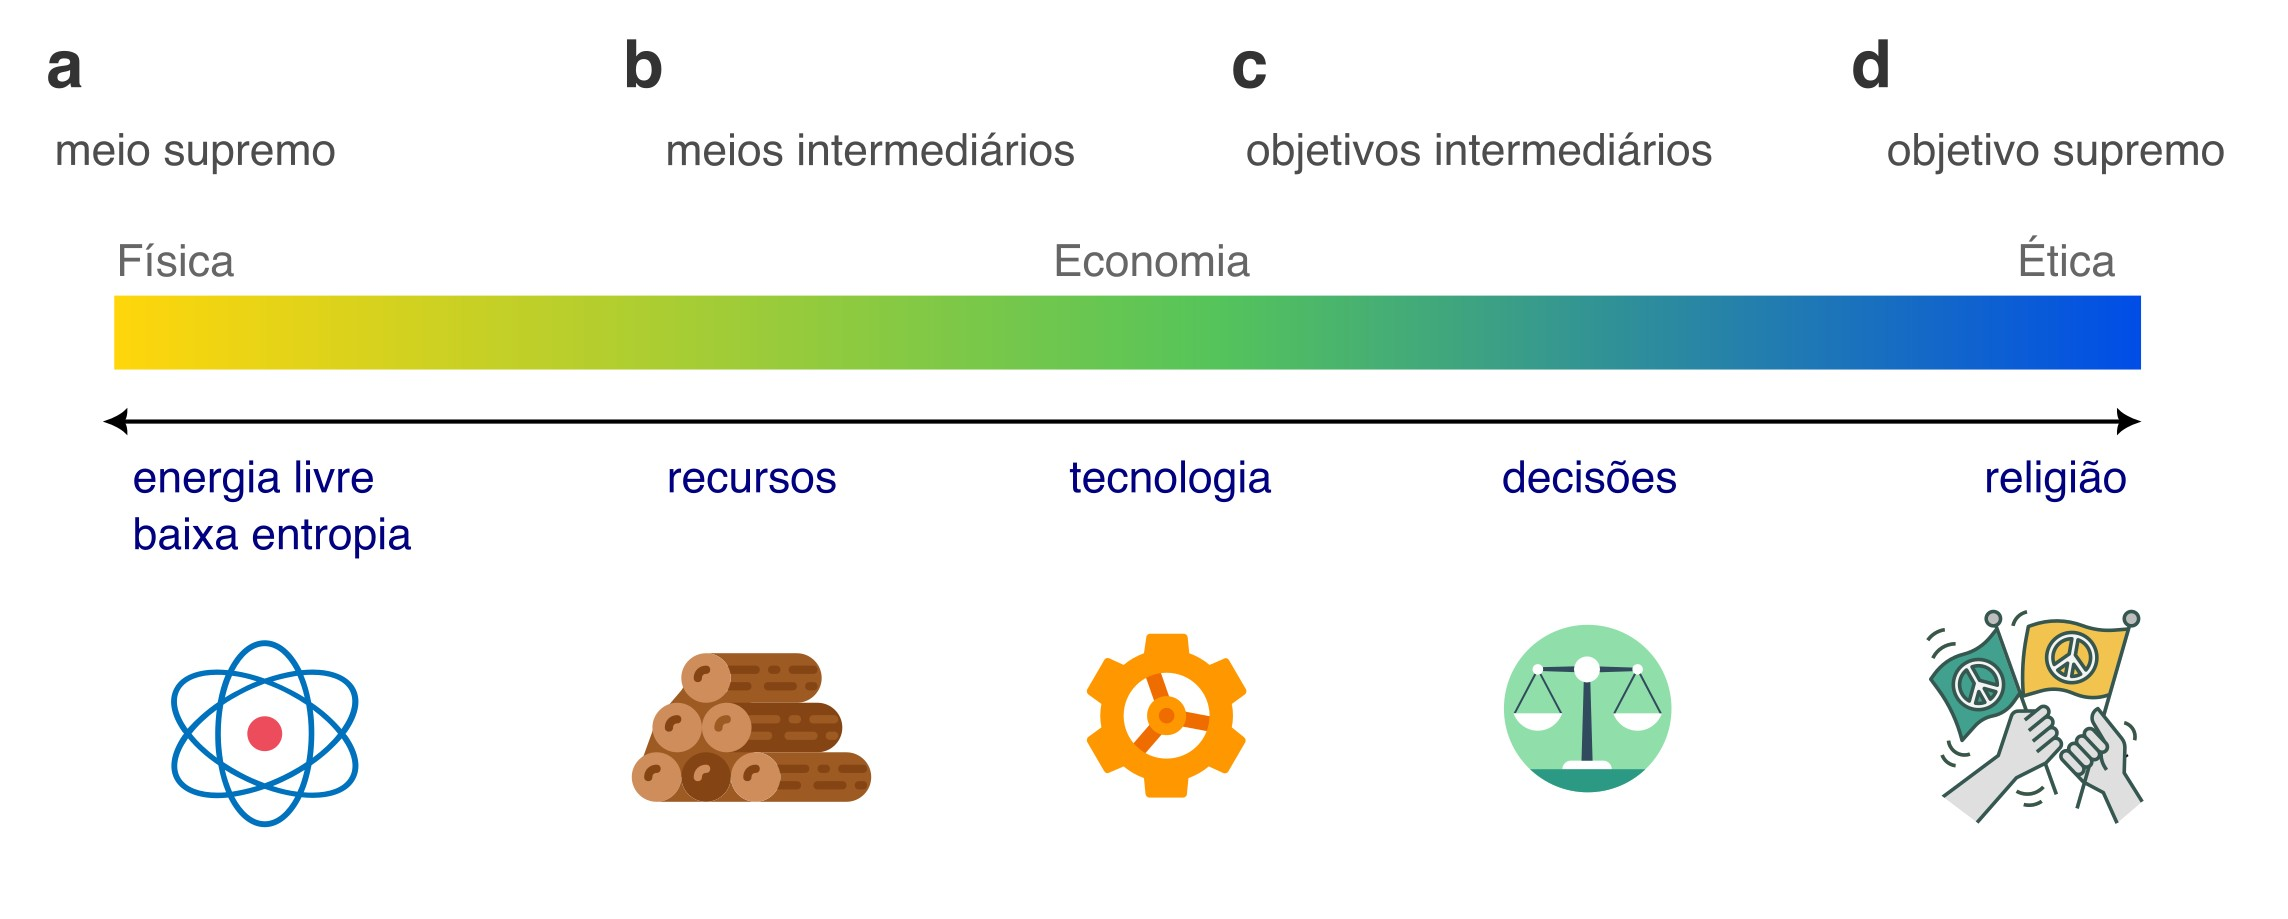
\includegraphics[width=0.98\linewidth]{figs/fig_economics.jpg}		
\caption[O espectro da Economia]
{\textbf{---\;O espectro da \gls{gseconomics}.}
    A Economia, sendo a alocação de recursos escassos entre diferentes objetivos, consiste na conexão entre recursos (meios) e objetivos (fins). \;\textbf{a}\;---\;A energia livre e materiais com baixa entropia são os meios supremos.
    \;\textbf{b}\;---\;Energia e materiais se manifestam por meios intermediários: recursos naturais e recursos transformados pela tecnologia.
    \;\textbf{c}\;---\;Decisões baseadas no emprego da tecnologia orientam a alocação dos recursos intermediários para atender objetivos intermediários.
    \;\textbf{d}\;---\;As decisões orientam-se por alguma religião, conjunto de valores éticos que visam algum objetivo supremo, explícito ou não.}
\label{fig:eco:economics} 		
\end{figure}

\par A \textbf{\gls{gseconomics}} é a ciência que se dedica ao estudo da alocação de recursos escassos entre diferentes objetivos. Por exemplo, podemos optar por utilizar aço na construção de casas ou de mísseis; destinar água para irrigação agrícola ou geração de energia; usar a terra para manter florestas tropicais de pé ou para criar e abater vacas. Qual é a melhor opção? Se os recursos citados são realmente escassos, essas opções não são meras falsas dicotomias falaciosas, mas questões muito sérias, com consequências drasticamente diferentes entre uma escolha e a outra. Nesse sentido, a \gls{gseconomics} não está somente associada à existência de recursos escassos, mas também está intrinsecamente ligada ao processo de tomada de \textbf{decisões}, de fazer escolhas, pois não se pode ter tudo ao mesmo tempo. Disso, a seguinte pergunta central se impõe:

-- Quais são os objetivos que guiam as escolhas?

\noindent Esta claramente não é uma pergunta empírica. Ela não pode ser respondida fazendo-se uma expedição de campo e testando hipóteses contra as evidências observadas, como são as perguntas sobre problemas científicos. Nesse caso, o mundo empírico simplesmente ofereceria uma confusão de respostas contraditórias. Tampouco é uma pergunta Lógica, que pode ser respondida a partir de axiomas fundamentais, como na Geometria. A pergunta revela-se, portanto, essencialmente \textbf{\gls{gsethics}}: ela pressupõe um valor moral daquilo que \textit{deve} ser objetivado\footnote{Esse tipo que questão também denomina-se \textbf{normativa}.}. A \gls{gsethics} é o ramo da Filosofia que explora os princípios e valores que orientam o comportamento humano, buscando definir o que é considerado certo ou errado, justo ou injusto, o que deve ser feito e aquilo que não deve ser feito. Por isso, a pergunta central da \gls{gseconomics} depende de uma orientação ética, fazendo dessa ciência uma ponte que conecta os meios (recursos) com os fins (objetivos), como ilustrado na Figura \ref{fig:eco:economics}. No âmbito estrito da Biologia, é claro, todos os organismos precisam lidar com a alocação de recursos escassos para endereçar o \textbf{\gls{existimper}}, que não tem nada a ver com \gls{gsethics}. Esse imperativo consiste em um objetivo bem nítido: para existir, é preciso tomar decisões para \textit{continuar} existindo. Assim, o \gls{ultimategoal} de um ser vivo é metabolizar e se reproduzir, por definição. Em termos humanos, isso implica obter as condições mínimas para a sobrevivência, como alimento, água, roupas, higiene, abrigos físicos e, sobretudo, relações sociais.

\par Ao contrário dos outros seres vivos, o historiador Yuval Harari sugere que os \textit{Homo sapiens}  instanciam \textbf{religiões} que definem objetivos existenciais além da mera sobrevivência \cite{harari2015sapiens}. As religiões são ficções coletivas, realidades intersubjetivas, que existem apenas no imaginário compartilhado entre pessoas de um dado grupo. Nesse sentido, as religiões definem o arcabouço ético que os seres humanos guiam as suas escolhas. Os processos históricos do Renascimento e da Modernidade fizeram surgir na Europa Ocidental o \textbf{\gls{gshumanism}}, uma religião que é hoje largamente influente no mundo. Em contraste com as religiões anteriores, que cultuavam entidades sobre-naturais, o \gls{gshumanism} se expressa sob uma forma de \textbf{\gls{antropoc}}, pois enfoca o próprio ser humano como o centro de todos os nossos objetivos \cite{lamont1997philosophy}. Um exemplo da transformação implicada pelo \gls{gshumanism} pode ser encontrado no \textit{Discurso do método} de René Descartes, onde o filósofo propõe que a busca da verdade deve ir além de uma compreensão teórica da realidade, mas também encontrar aplicações práticas que melhorem a condição humana \cite{descartes2008discurso}. Na mentalidade medieval, por outro lado, essa concepção era inacessível, já que o conhecimento objetivava entender a obra de Deus e a miserável condição humana seria salva somente após a morte. Outras religiões eventualmente assumem que a nossa miséria relaciona-se com reincarnações, etc. Pelo prisma político, o \gls{gshumanism} fez surgir diversas sub-religiões, ou doutrinas, tais como o Liberalismo, que cultua o \say{indivíduo}, o Socialismo, que cultua a \say{sociedade}, e o Fascismo, que cultua a \say{nação}\footnote{Essas doutrinas obviamente não são rígidas, existindo em um gradiente e combinações inusitadas entre si e com outras religiões tradicionais. Por exemplo, o Socialismo pode ser influenciado pelo Liberalismo, como visto na União Europeia, ou influenciado pelo Fascismo, como visto na União Soviética.}. Mas principalmente, o \gls{gshumanism} também fez surgir o \textbf{\gls{gnaturalism}} moderno, uma \gls{teoria} realista que sustenta que nada existe fora do mundo natural e, portanto, qualquer explicação sobre a realidade deve ser encontrada dentro do próprio Universo.

\subsection{A Ética do Utilitarismo} \label{subsec:bentham}

\par No campo da \gls{gsethics}, uma corrente filosófica dentro do \gls{gshumanism} é o \textbf{\gls{gutilitarism}} de Jeremy Bentham (1748-1832) \cite{Gordon2002a}. Esse filósofo propõe que a moralidade de uma ação deve ser determinada pelas suas consequências, com foco na maximização do \textbf{\gls{welbeing}} do maior número possível de indivíduos. Para Bentham, o princípio fundamental que orienta a avaliação moral é o da \textbf{\gls{gutility}}, entendido como a capacidade de uma ação em aumentar ou diminuir o prazer e a dor daqueles que são afetados por ela. Bentham define \gls{welbeing} como a predominância do prazer sobre a dor, e argumenta que todas as ações humanas são motivadas por esses dois fatores. Ele desenvolve um método de avaliação, conhecido como \textbf{\gls{hedonacc}}, que permite medir o impacto moral de uma ação levando em conta aspectos como a intensidade, a duração, a certeza, a proximidade e a extensão dos prazeres e dores envolvidos. Esse cálculo visa quantificar o bem-estar gerado pelas ações e orientar as escolhas morais. O \gls{gutilitarism} de Bentham, portanto, adota uma perspectiva tida como consequencialista e imparcial, onde a correção de uma ação depende dos seus resultados práticos, e não das intenções do agente. Além disso, essa \gls{teoria} considera que o bem-estar de todos os afetados deve ser ponderado de maneira equitativa. Assim, a ação moralmente correta é aquela que promove o máximo de prazer e o mínimo de dor para o maior número de pessoas, sendo essa a métrica final para julgar o valor moral das ações. 

\par De longe, o \gls{gutilitarism} de Bentham faz sentido. Dentro do \gls{gshumanism}, é intuitiva e natural a ideia de maximizar o \gls{welbeing}, de guiar as decisões para evitar a dor e buscar o prazer. No entanto, essa \gls{teoria} ética é vaga o suficiente para permitir interpretações diversas, o que leva a orientações políticas e econômicas muito diferentes na prática. Teoricamente, o Liberalismo, o Socialismo e o Fascismo são utilitaristas de uma forma ou de outra, embora a materialização de suas ideias durante o século XX tenha resultado em economias e regimes políticos bastante distintos. No Liberalismo, parte-se do princípio de que, se cada indivíduo for livre para maximizar o próprio bem-estar, o bem-estar geral aumentará por uma espécie de auto-regulação. No Socialismo, assume-se que o bem-estar coletivo crescerá mediante a regulação ou gestão do Estado na economia. No Fascismo, acredita-se que o bem-estar geral da nação será maximizado desde que os indivíduos ou grupos considerados traidores ou impuros sejam expulsos (ou coisa pior). 

\par Para complicar, o \gls{gutilitarism} enfrenta desafios com uma base científica muito frágil. As teorias psicológicas e neurológicas modernas sugerem que é impossível ampliar indefinidamente uma sensação subjetiva. A \textbf{\gls{adaplevel}}, por exemplo, estabelece que estímulos emocionais constantes são transferidos para um plano de fundo mental, onde são então ignorados, fato que liberta recursos mentais para que \textit{novidades} sejam adequadamente contempladas \cite{Edwards_2018}. Seguindo essa linha, a busca por mais bem-estar conduz os seres humanos para uma \textbf{\gls{hedonmill}}, uma forma de insatisfação existencial crônica e viciante em que, mesmo diante de melhorias constantes no conforto material e experiências recompensadoras, o nível de bem-estar tende a retornar ao um nível de base fixo, frustrando a busca por uma felicidade duradoura e crescente \cite{Diener2009}. Evidências empíricas corroboram essa tese, como em situações em que vencedores de loterias (evento positivo) e desabilitados por acidentes (evento negativo) retornam ao seu nível de base após o evento \cite{Brickman_1978}. Como a neurociência sustenta que dor e prazer são processos fundamentalmente materiais (sinapses), esses estados psicológicos e fisiológicos não podem crescer de forma indefinida, o que torna problemática a ideia de \say{maximização do bem-estar humano}\footnote{A neurociência estabelece que pensamentos são sinapses. Sem sinapses, pensamentos não existem. Porém, a neurociência não explica a \textit{manifestação subjetiva} que acompanha as sinapses. Esse é conhecido como o \gls{consproblem}.}.

\par A \gls{gseconomics} incorporou profundamente o conceito de maximização da \gls{gutility} como \textbf{\gls{ultimategoal}}, que serve de base tanto para a \textbf{\gls{microeon}}, que busca explicar o funcionamento de mercados específicos e as interações entre consumidores e produtores, quanto para a \textbf{\gls{macroeon}}, que visa entender a economia em sua totalidade, abrangendo desde o nível nacional até a economia global. No entanto, as doutrinas clássicas dessas teorias, desenvolvidas no século XIX, embora científicas, enfrentaram dificuldades em se sustentar empiricamente ao longo do tempo. Teóricos começaram a questionar suas suposições fundamentais ainda no século XIX, e essas críticas se intensificaram ao longo do século XX. Na \gls{microeon}, a versão clássica foi revisada por correntes como a \textbf{\gls{microeon} Evolutiva}, que expande os conceitos clássicos ao introduzir a racionalidade limitada, o comportamento dinâmico e as interações institucionais \cite{Nelson1985a, Bourgine2006a}. Essa abordagem busca explicar fenômenos mais complexos e realistas, como a dispersão de preços e a diversidade das estruturas industriais, que a \gls{teoria} clássica, baseada na racionalidade perfeita e no equilíbrio estático, tinha dificuldade em abordar. Já no campo da \gls{macroeon}, a crítica à versão clássica foi ainda mais radical. Proponentes da \textbf{\gls{ecoeco}}, como Herman Daly (1938-1922), rejeitam completamente a doutrina clássica e neoclássica da \gls{macroeon}, argumentando que ela negligencia as leis da termodinâmica. Como veremos mais adiante, a \gls{ecoeco} propõe uma legítima mudança de \gls{paradigma}, colocando a sustentabilidade no centro das análises macroeconômicas e destacando que o \gls{ecogrowth} ilimitado é inviável em um planeta com recursos finitos.

\subsection{A teoria da utilidade marginal} \label{subsec:marginutil}

\begin{figure}[t!] 
\centering				
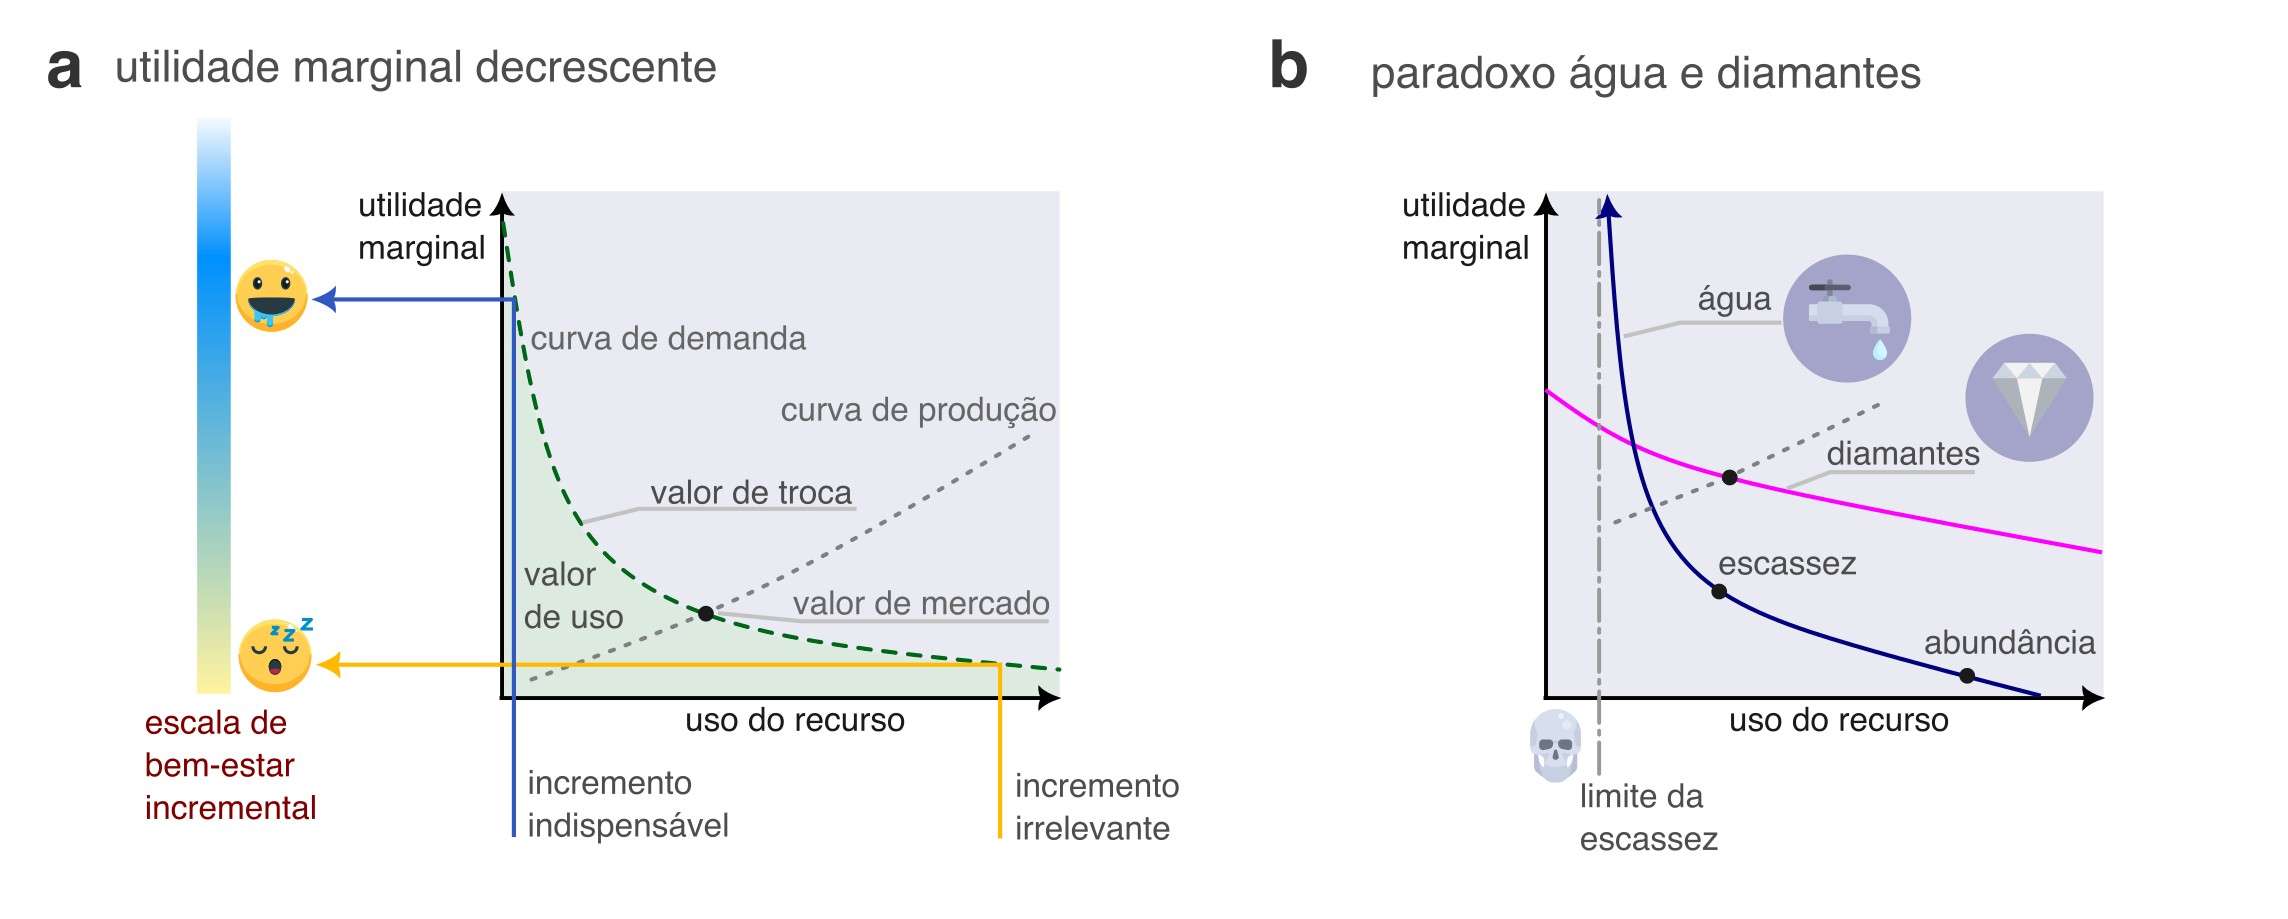
\includegraphics[width=0.98\linewidth]{figs/fig_marginalutil.jpg}		
\caption[Utilidade marginal e as curvas de demanda]
{\textbf{---\;Utilidade marginal e as curvas de demanda.}
    A teoria da utilidade marginal explica o sistema de preços observado em mercados. A utilidade marginal, assim, é equivalente ao valor de troca dos recursos. 
    \;\textbf{a}\;---\;A teoria se fundamente no princípio da utilidade marginal decrescente, o conceito de que o agente econômico consumir sacia-se cada vez mais à medida que consome um dado recurso, formando uma curva de demanda com declividade negativa. Inicialmente, as primeiras unidades consumidas produzem uma grande utilidade marginal, é um incremento de consumo indispensável. Mas a utilidade marginal diminui ao passo que os incrementos de consumo tornam-se irrelevantes. A curva de produção desse recurso no lado da oferta estabelece o ponto em produtores e consumidores estão igualmente satisfeitos, formando o preço de mercado.
    \;\textbf{b}\;---\;A teoria da utilidade marginal explica o valor de troca em condições de escassez e abundância. A água, essencial à vida, possui baixa utilidade marginal e valor de mercado quando abundante, mas em escassez, sua utilidade marginal cresce, tornando-a valiosa. Em contraste, diamantes, que não são essenciais, mantêm alto valor de mercado devido à sua escassez. O limite de escassez indica o ponto em que a utilidade marginal de recursos essenciais como a água atinge níveis críticos, elevando seu valor de troca muito acima de recursos não essenciais.
}
\label{fig:eco:marginutil} 		
\end{figure}

\par Na \gls{microeon}, o \gls{gutilitarism} encontrou sua expressão máxima na \textbf{\gls{marutilteo}} durante o século XIX, articulada por pensadores como William Stanley Jevons e Carl Menger \cite{Gordon2002a}. Essa \gls{teoria} busca explicar os preços em mercados, entendidos como o resultado de milhares de decisões independentes e descentralizadas entre consumidores e produtores. Ou seja, em um \gls{system} de livre-mercado, a informação sobre a escassez de um recurso é transmitida aos consumidores por meio de seu \textbf{\gls{gprice}}. A \gls{marutilteo} sustenta que o \gls{gprice} de um bem ou serviço consiste no \textbf{valor de mercado}, ou \textbf{\gls{exchaval}}, em condições que satisfazem tanto os produtores quanto os consumidores (ver Figura \ref{fig:eco:marginutil}\textbf{a}). Esse valor corresponde à \gls{gutility} adicional que um indivíduo obtém ao consumir uma unidade extra de um bem, a qual diminui conforme o consumo aumenta — o denominado \textbf{\gls{prindecmarut}}. Em termos práticos, isso significa que o consumidor tende a se \textit{saciar} à medida que consome mais de um determinado bem ou serviço, produzindo uma curva de demanda com declividade negativa. 

\par A \gls{teoria} explica com relativo sucesso o chamado \textbf{\gls{waterdiamonds}}, a bizarra diferença de valor entre diamantes (pouco útil) e água (muito útil) (ver Figura \ref{fig:eco:marginutil}\textbf{b}).  Nesse caso, o \textbf{\gls{useval}} de um recurso essencial para a sobrevivência como a água pode ser extremamente alto, enquanto seu \gls{exchaval} é relativamente baixo, especialmente onde a água é abundante. Por outro lado, bens como diamantes ou joias têm um \gls{useval} baixo, mas possuem um \gls{exchaval} elevado devido à sua escassez e à alta demanda por aqueles que as consideram itens de status social (mas o \gls{exchaval} é baixo em sociedades que preferem um cocar de penas, por exemplo). Em uma situação de escassez extrema de água, por outro lado, o \gls{exchaval} da água facilmente superar o valor dos diamantes, pois torna-se uma questão de vida ou morte. Esse contraste ilustra como o \gls{useval} e o \gls{exchaval} podem divergir significativamente, e como a \gls{gutility} marginal ajuda a explicar o \gls{gprice} de mercado, independentemente da funcionalidade do bem ou serviço.\footnote{A Teoria do Valor-Trabalho de Karl Marx contrasta com a \gls{marutilteo} ao afirmar que o \textbf{\gls{workval}} de um bem é determinado pelo trabalho socialmente necessário para produzi-lo, e não pela \gls{gutility} que o bem proporciona ao consumidor. Segundo Marx, o valor de um bem é proporcional à quantidade de trabalho incorporado em sua produção, o que inclui tanto o trabalho direto quanto o trabalho necessário para produzir os meios de produção. Esse conceito fundamenta a análise de Marx sobre a exploração do trabalho para se acumular capital, onde os bens são trocados com base no valor do trabalho, mas os trabalhadores recebem apenas uma fração desse valor, criando a mais-valia, ou lucro, para os proprietários dos meios de produção. Ainda que o \gls{workval} de um bem ou serviço possa existir, o problema da tese marxiana é que, na prática, os bens produzidos pelos trabalhadores são vendidos em mercados, pelo \gls{exchaval} auferido pelos consumidores.} Com base nessa lógica, a \gls{teoria} fornece um \gls{model} para explicar (e prever) a formação dos preços nos mercados, e seu conceito de \textbf{\gls{pareteff}} sugere que, sob certas condições, os mercados atingem um equilíbrio, alocando recursos escassos de forma otimizada a satisfazer a todos, sem que seja possível melhorar a situação de alguém sem prejudicar outro.

\par O poder explicativo da \gls{marutilteo} parece corroborar o conceito de \gls{gutility}, já que consumidores e produtores em mercados reais supostamente ajustam suas decisões de acordo com os benefícios marginais -- mesmo sem nunca terem ouvido falar de Jeremy Bentham ou de \gls{gutility} marginal decrescente. Junto com outras teorias auxiliares, a \gls{marutilteo} compõe a base da \gls{microeon} Clássica, que busca explicar cientificamente o funcionamento geral de mercados específicos. Esse conjunto de teorias assume que os agentes na economia são plenamente racionais, capazes de maximizar a sua \gls{gutility} individual, e que os mercados funcionam de maneira eficiente para maximizar a \gls{gutility} total, alcançando um equilíbrio de forma automática, sem intervenções externas. No entanto, para que a suposta eficiência na alocação de recursos seja alcançada, é necessário que não existam \textbf{\gls{marketdist}}, e que condições ideais estejam presentes, como a existência de muitos produtores, disponibilidade total de informações e a ausência de especulação e propaganda — fatores que raramente se verificam na realidade. Além das \gls{marketdist}, o comportamento irracional dos seres humanos, como demonstrado por Daniel Kahneman \cite{kahneman2011}, desafia a ideia de mercados completamente eficientes. Consumidores e produtores, influenciados por vieses cognitivos, como a aversão à perda e o viés de ancoragem, muitas vezes tomam decisões não inteiramente racionais, gerando ineficiências e distorções nos preços. 

\par A \gls{microeon} Evolutiva tenta superar essas limitações ao adotar uma abordagem mais dinâmica, incluindo principalmente simulações com \gls{abm-models} \cite{Bourgine2006a}. Nesse caso, os agentes possuem racionalidade limitada e informações locais, e suas interações ocorrem ao longo do tempo, em processos definidos explicitamente. Além disso, várias instituições, além do mercado, influenciam e sustentam a alocação dos recursos. Assim, a microeconomia evolutiva oferece uma explicação teórica mais robusta para fenômenos que a microeconomia clássica tem dificuldade em justificar. Os \gls{abm-models} da abordagem evolutiva, naturalmente caóticos e computacionalmente irredutíveis, deixam mais claro que, embora ambicionem realizar previsões, as teorias micro-econômicas geralmente se limitam a modelagens exploratórias. Os modelos, assim, trazem uma ampla \gls{explan_cap}, mas pouca \gls{pred_cap}, fazendo a adequação empírica ocorrer em casos muito específicos, geralmente favorecendo algumas das \gls{aux-hyp}, mas não o \gls{model} em sua completude.

\subsection{Paradigmas macroeconômicos} \label{subsec:macroeco}

\par Como mencionado anteriormente, a \gls{macroeon} se diferencia da \gls{microeon} por buscar explicar a economia como um todo, indo além de mercados específicos e abrangendo até a economia nacional e global \cite{samuelson2009}. As doutrinas clássica e neoclássica da \gls{macroeon}, no entanto, tendem a ser uma generalização da \gls{microeon}, expandindo a visão para todos os mercados, produtores e consumidores em uma região de interesse, como um país. O \gls{model} macroeconômico clássico consiste no \textbf{\gls{circflowexval}} entre produtores e consumidores. Na prática, isso corresponde ao fluxo de \gls{exchaval} entre empresas e domicílios, que pode ser medido anualmente pelo faturamento total das empresas e pela renda dos domicílios. Como se trata de um fluxo circular, o valor total de um deve ser equivalente ao do outro. 

\par A escola Neoclássica revisa o \gls{model} clássico ao inserir no \gls{circflowexval} as injeções e vazamentos causados pelas finanças privadas (investimentos e reservas individuais), finanças públicas (arrecadação de impostos e investimentos públicos) e finanças internacionais (importações e exportações). A maximização da \gls{gutility} total, tido como o \gls{ultimategoal}, pode ser entendida como a maximização desse fluxo de \gls{exchaval} no \gls{system} circular. Portanto, a escola Neoclássica se foca unicamente no fluxo de \gls{exchaval} nos mercados e nas estratégias para aumentá-lo, o que é chamado de \textbf{\gls{ecogrowth}}. As diferenças entre essas estratégias variam, geralmente envolvendo mais ou menos regulação ou intervenção estatal nos mercados de forma a reduzir o desemprego e estabilizar preços. Políticas fiscais e monetárias, por sua vez, objetivam controlar de alguma forma os vazamentos dos impostos e reservas individuais. O sucesso de uma estratégia, porém, é testado pelo aumento no faturamento das empresas ou na renda dos domicílios, sendo esse crescimento interpretado como um sinal de progresso em direção ao \gls{ultimategoal} de maximizar a \gls{gutility} total.

\par A \gls{ecoeco}, articulada principalmente por Herman Daly, propõe um novo \gls{paradigma} que rejeita a escola Neoclássica \cite{daly2011}. Essa visão propõe a \gls{teoria} macroeconômica seja incorporada à \textbf{\gls{ecology}}, uma ciência baseada em princípios físicos, reconhecendo que o \gls{sys-target} a ser modelado é, essencialmente, um \gls{system} material \cite{Daly1968a}. Ao que consta, a perspectiva material sobre a \gls{gseconomics} estava presente nas suas origens modernas, mas foi lentamente sendo substituída pelo interesse no \gls{exchaval}, que é imaterial \cite{Christensen1987}. Um bom exemplo é o de Thomas Malthus (1766-1834), que identificou potenciais limites para o crescimento da população humana em função da produção de alimentos, que cresceria a um ritmo relativamente mais lento. Em essência, Malthus via claramente os seres humanos como seres materiais, que precisam de nutrientes e energia para sobreviver, assim como qualquer outra espécie no planeta. Por exemplo, se um ser humano precisa consumir diariamente 3 litros de água e 0,4 kg de alimentos (aproximadamente 2000 calorias, divididas entre gorduras, carboidratos e proteínas), então se deduz que a população global atual de 8 bilhões de pessoas demanda diariamente 24 milhões de metros cúbicos de água e 50 mil toneladas de alimentos. Sem um fluxo material dessa magnitude, a população global não duraria muito tempo. Oito bilhões parece bastante gente, mas será que seria possível dobrar esse tamanho? Ou triplicar?

\par Uma vez que as previsões de fome generalizada e colapso populacional de Malthus não se concretizaram em sua época, economistas clássicos e neoclássicos tendem a desconsiderar sua \gls{teoria}, confundindo suas conclusões circunstanciais com os fundamentos materiais de sua abordagem. No debate acirrado que surgiu com a proposta da \gls{ecoeco}, economistas neoclássicos acusam os proponentes do novo \gls{paradigma} de serem \say{neomalthusianos}, o que soa um tanto de forma pejorativa \cite{Forrester1974}. A visão ecológica, por sua vez, acusa a escola Neoclássica em se focar excessivamente nos fluxos de \gls{exchaval} de \textbf{\gls{marktegoods}}, bens e serviços muito específicos que podem ser comprados ou vendidos \cite{Daly1997a, Daly1997b}. Esse foco no fluxo de valor é tão hegemônico que a escola Neoclássica sequer considera a materialidade das \gls{marktegoods}: elas são apenas \textit{veículos} que transportam \gls{gutility} marginal, definida pelo seu \gls{gprice}. Assim, a escola Neoclássica instancia uma ontologia imaterial e abstrata de \gls{exchaval}. Essa representação pode ser um \gls{model} interessante para entender e explicar os fluxos de valores em mercados, mas nem de perto consiste em uma representação de uma realidade material.

\subsection{A ontologia do Fisicalismo} \label{subsec:physicalism}

\par Em termos ontológicos, a \gls{ecoeco} sustenta uma realidade fisicalista. O \textbf{\gls{gphysicalism}}\footnote{Também denominado de Materialismo.} é uma corrente de pensamento realista e naturalista que postula que a realidade objetiva existe, rege-se pelas leis da Física e é composta em última instância de matéria e energia \cite{sep-physicalism}. Sendo a Física uma \gls{teoria} científica, o \gls{gphysicalism} consiste na principal visão de mundo diretamente implicada pelo Realismo Científico. Nessa perspectiva, até mesmo o conceito de \gls{gutility} consiste em algo material, pois coisas como \say{bem-estar} ou \say{satisfação} na verdade são sinapses em cérebros, um órgão do corpo humano. 

\par O \gls{gphysicalism}, apesar de atrativo devido à sua forte adequação empírica, enfrenta alguns problemas estruturais críticos. Um dos principais é o problema mente-corpo, ou o \textbf{\gls{consproblem}} — a aparente impossibilidade de se explicar as experiências subjetivas a partir de processos físicos, como as sinapses \cite{sep-consciousness}. Outro problema grave é o \textbf{\gls{willproblem}}, que surge ao se aceitar as últimas consequências do \gls{gphysicalism}, que é o Determinismo \cite{sep-skepticism}. Em uma realidade determinista, decisões seriam meras sensações, sem agência real, tornando a ideia de escolhas na alocação de recursos, central na \gls{gseconomics}, desprovida de qualquer sentido\footnote{O \gls{gphysicalism} radical conduz ao Niilismo, uma \gls{teoria} ética que nega a existência de valores morais ou objetivos supremos para orientar decisões}. Mas ambos os problemas são sintomas do Realismo Científico, que propõe que a Ciência busca descrever a verdade sobre a realidade. Os Instrumentalistas, como Bas van Fraassen e Nancy Cartwright, contestam essa visão, argumentando que as teorias científicas objetivam apenas produzir descrições \textit{empiricamente adequadas}, sem necessariamente refletir a verdade última sobre o mundo \cite{bas1980, nancy1983}. Nesse sentido, escolher uma ontologia fisicalista para a \gls{macroeon} oferece uma base empiricamente mais robusta do que a escola Neoclássica, cuja explicação se limita ao fluxo de \gls{exchaval} nos mercados. Verdadeira ou não, uma base física oferece maior \gls{explan_cap} e preditiva do que o \gls{model} de fluxo circular neoclássico.

\par Um dos pioneiros a aceitar e difundir o \gls{gphysicalism} na \gls{gseconomics}, preparando o terreno para o \gls{paradigma} ecológico, foi Nicholas Georgescu-Roegen (1906-1994), especialmente com sua obra seminal \textit{A Lei da Entropia e o Processo Econômico}\footnote{Tradução livre de \textit{The Entropy Law and the Economic Process}} (1971). Nessa obra, Georgescu-Roegen destaca as implicações da primeira e da segunda leis da termodinâmica em uma economia baseada em recursos materiais. A \textbf{\gls{firstlaw}}, conhecida como o \textbf{princípio da conservação}, afirma que matéria e energia não podem ser criadas nem destruídas, apenas transformadas de uma forma para outra. Já a \textbf{\gls{secondlaw}} estabelece que a \textbf{entropia} de um \gls{system} isolado tende a aumentar, indicando que os processos naturais seguem uma trajetória de desordem crescente. Isso significa que a \textbf{energia livre}, capaz de realizar trabalho, tende a se degradar em formas cada vez menos capazes de realizar trabalho. Da mesma maneira, as estruturas materiais tendem a se desintegrar espontaneamente de um estado ordenado (heterogêneo e menos provável) para um estado desordenado (homogêneo e mais provável). A segunda lei implica também que nenhum processo de transferência de energia ou conversão material é 100\% eficiente, pois sempre ocorrerão perdas na forma de calor e resíduos. Portanto, essas leis estabelecem que a manutenção de ordem no Universo só é possível localmente e às custas de fontes externas de energia livre. Mesmo assim, a criação de ordem por meio de trabalho resulta inevitavelmente na geração de resíduos materiais e energéticos sem \gls{gutility}.

\par Outro pioneiro na visão fisicalista foi Jay Forrester, o inventor da \gls{sys-dyn}, tema introduzido no Capítulo \ref{chap:systems}. Jay Forrester e a sua equipe de engenheiros e cientistas no \texttt{MIT} demonstraram a partir das publicações \textit{World Dynamics} e \textit{Limites do crescimento} como que modelos de compartimentos podem ser empregados para se obter previsões sobre o estado da economia global ao longo do tempo \cite{Forrester1973a, meadows1974}. As simulações do \gls{model} \texttt{World3} introduziram uma abordagem fisicalista, demonstrando a materialidade do \gls{system} econômico ao integrar os níveis e fluxos materiais dos \gls{system} global, tais como a população, capital industrial, terras agricultáveis e a poluição resultante. Os resultados, ainda que variados para diferentes cenários, evidenciam os limites físicos impostos pela \gls{biosf} sobre a \gls{antroposf}, como o esgotamento de fontes energéticas não-renováveis, a degradação de terras agrícolas e a capacidade finita de absorção de poluentes dos ecossistemas. Nos diversos cenários explorados, o crescimento da população humana e de capital industrial enfrentam inevitavelmente um ponto de ruptura, onde o aumento dos custos de extração de recursos, a perda de produtividade agrícola e os impactos da poluição aplicam retroações negativas cada vez maiores, resultando cedo ou tarde em um declínio no crescimento de capital industrial. Assim, as explorações do \texttt{World3} ilustraram a interdependência entre o \gls{system} econômico e os limites físicos da \gls{biosf}.

\subsection{O modelo ecológico de macroeconomia} \label{subsec:ecomodel}

\begin{figure}[t!] 
\centering				
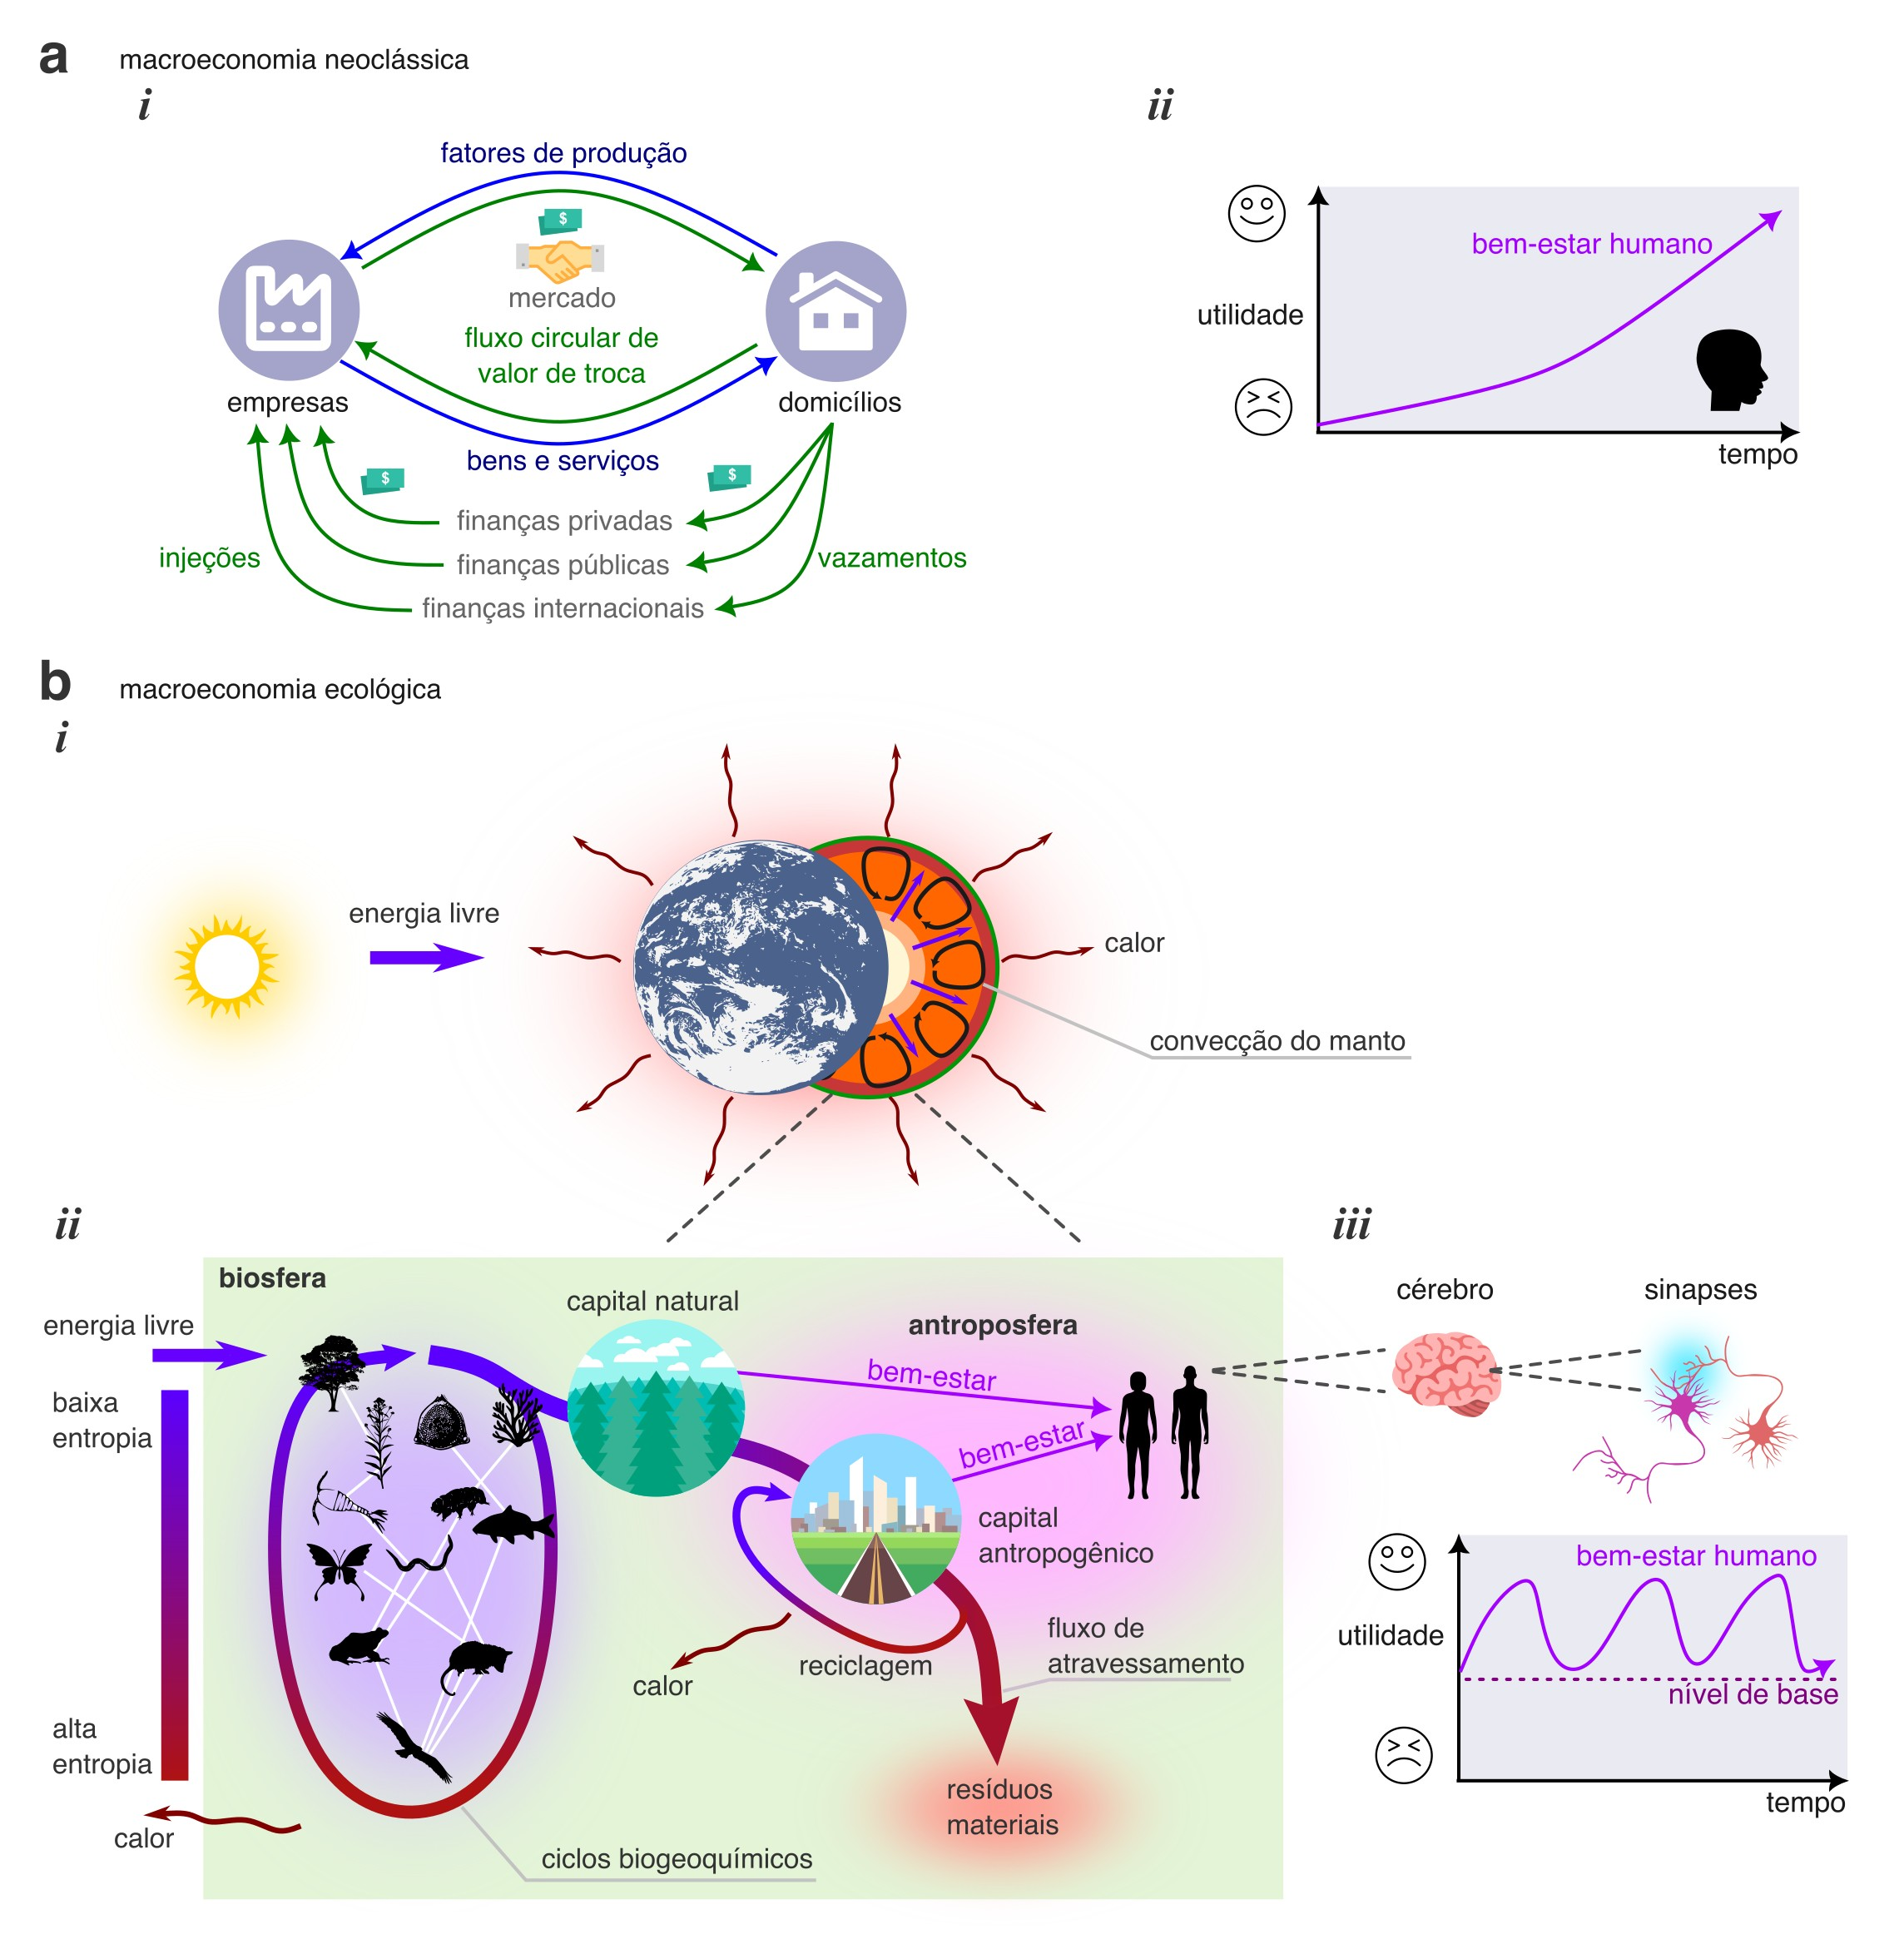
\includegraphics[width=0.98\linewidth]{figs/fig_ecomodel.jpg}		
\caption[A \gls{macroeon} Ecológica]
{\textbf{---\;A \gls{macroeon} ecológica.}
    Ao contrário da macroeconomia neoclássica, a macroeconomia ecológica instancia um modelo baseado nas leis da termodinâmica.     
    \;\textbf{a}\;---\;O modelo neoclássico de macroeconomia busca representar um fluxo circular de valor de troca entre empresas e domicílios, com injeções e vazamentos gerados pelas políticas fiscais e financeiras de agentes privados e públicos (detalhe \textrm{\textit{i}}). Se o fluxo de valor de troca aumenta, a utilidade aumenta, pois o valor de troca é equivalente à utilidade marginal. Com isso, se conclui que o aumento do fluxo de valor de troca é um indicador direto aumento do bem-estar humano (detalhe \textrm{\textit{ii}}).    
    \;\textbf{b}\;---\;O modelo ecológico de macroeconomia admite uma ontologia fisicalista, que instancia fluxos de matéria e energia em sistemas abertos. A biosfera é a camada superior da Terra que lentamente troca matéria com o manto e recebe fluxos de energia livre do Sol e do núcleo, emitindo calor para o espaço (detalhe \textrm{\textit{i}}). O fluxo de energia livre na biosfera é processado por ciclos biogeoquímicos, incluindo ecossistemas, circulando materiais entre os extremos de baixa e alta entropia. A antroposfera consiste no habitat humano inserido dentro da biosfera e é atravessada por um fluxo linear de matéria, que resulta em resíduos (detalhe \textrm{\textit{ii}}). Nesse sistema, o bem-estar humano é também um processo material e finito, obtido tanto a partir do capital antropogênico, as estruturas da antroposfera, quanto diretamente do capital natural, as estruturas já existentes na biosfera (detalhe \textrm{\textit{iii}}).
}
\label{fig:eco:ecomodel} 		
\end{figure}

\par A partir das leis termodinâmicas e da visão sistêmica, a \gls{ecoeco} representa a macroeconomia por um \gls{model} ecológico, ilustrado na Figura \ref{fig:eco:ecomodel}. Nesse \gls{model}, a \textbf{\gls{antroposf}} – o ambiente material habitado pelos seres humanos – está inserida na \textbf{\gls{biosf}}, que abrange o \gls{system} material da superfície da Terra, desde a atmosfera até os primeiros quilômetros subterrâneos da litosfera. Energeticamente, a \gls{biosf} não é um \gls{system} isolado, mas aberto, recebendo um fluxo contínuo de energia livre da radiação do sol e do núcleo interno do planeta. Essa energia de alta qualidade, após realizar trabalho, é emitida para o espaço em formas menos úteis de calor. Materialmente, a \gls{biosf} também está conectada a fluxos de entrada e saída promovidos pelos processos de subducção, soterramento, soerguimento e vulcanismo, que resultam dos movimentos de convecção do manto, além das perdas de gases leves para o espaço. Embora processos como o vulcanismo representem exceções mais súbitas, a maioria das trocas materiais na \gls{biosf} ocorre de maneira extremamente lenta, em escalas geológicas. Dessa forma, a \gls{biosf} pode ser considerada, na prática, um \gls{system} energeticamente aberto, mas materialmente fechado.

\par A abertura energética de um \gls{system} é fundamental para a criação de ordem no seu interior. A fotossíntese, por exemplo, é um dos principais processos de geração de ordem na \gls{biosf}, ao empregar a energia livre da radiação solar para produzir materiais de baixa entropia, como açúcares, a partir de compostos de alta entropia, como o dióxido de carbono. Processos de soterramento desses materiais de baixa entropia ao longo de milhões de anos produziram as reservas de combustíveis fósseis amplamente utilizadas hoje pela \gls{antroposf}. Além da fotossíntese, o motor do ciclo do carbono, diversos outros \textbf{ciclos bio-geoquímicos} ocorrem na \gls{biosf}, todos impulsionados por fontes externas de energia. O \gls{hydro_cicle}, por exemplo, é movido pela energia solar, que evapora a água e a eleva, conferindo-lhe potencial gravitacional, que pode realizar trabalho em moinhos ou turbinas. Esses ciclos mantêm a dinâmica e a ordem da \gls{biosf}, demonstrando a interdependência entre o aporte de energia externa e a organização interna do \gls{system}.

\par Os fundamentos físicos da \gls{ecoeco} resulta em uma interpretação completamente diferente de \gls{ecogrowth}. A \gls{firstlaw}, vista sob a lente do \gls{model} ecológico, implica que não existe crescimento material real na \gls{biosf}, uma vez que a matéria se conserva. A \gls{antroposf}, sendo um habitat humano dentro da \gls{biosf}, pode expandir a sua complexidade estrutural ao processar os materiais da \gls{biosf}, mas sempre às custas da geração de calor e outros resíduos. A \gls{secondlaw}, por sua vez, implica que a mera \textit{sustentação} da atroposfera exige um fluxo de energia livre e de materiais de reposição, pois é necessário trabalhar continuamente contra a degradação espontânea do \gls{system} material. Esse fluxo inevitável de matéria que é processada pela \gls{antroposf} e gera resíduos inúteis dispersos na \gls{biosf} é chamado na \gls{ecoeco} de \textbf{\gls{gthoughput}}\footnote{Tradução livre de \textit{throughput}.}. Nesse sentido, o \gls{ecogrowth} teorizado pela \gls{gseconomics} Neoclássica é, sobretudo, uma ilusão, um fenômeno imaginário instanciado pela realidade intersubjetiva do \gls{exchaval}. Mas como bens e serviços em mercados são entidades materiais, aumentar o seu consumo implica, obrigatoriamente, em aumentar o \gls{gthoughput}. A diferença entre os paradigmas econômicos, aqui, torna-se muito clara: enquanto um instancia um fluxo circular e imaterial (\gls{gutility} marginal e valor de troca), o outro vê um fluxo linear e material (processamento de energia livre).

\section{Capital natural} \label{chap:ecoeco:natcap}

\subsection{A escala ótima da antroposfera} \label{subsec:escaleopt}

\begin{figure}[t!] 
\centering				
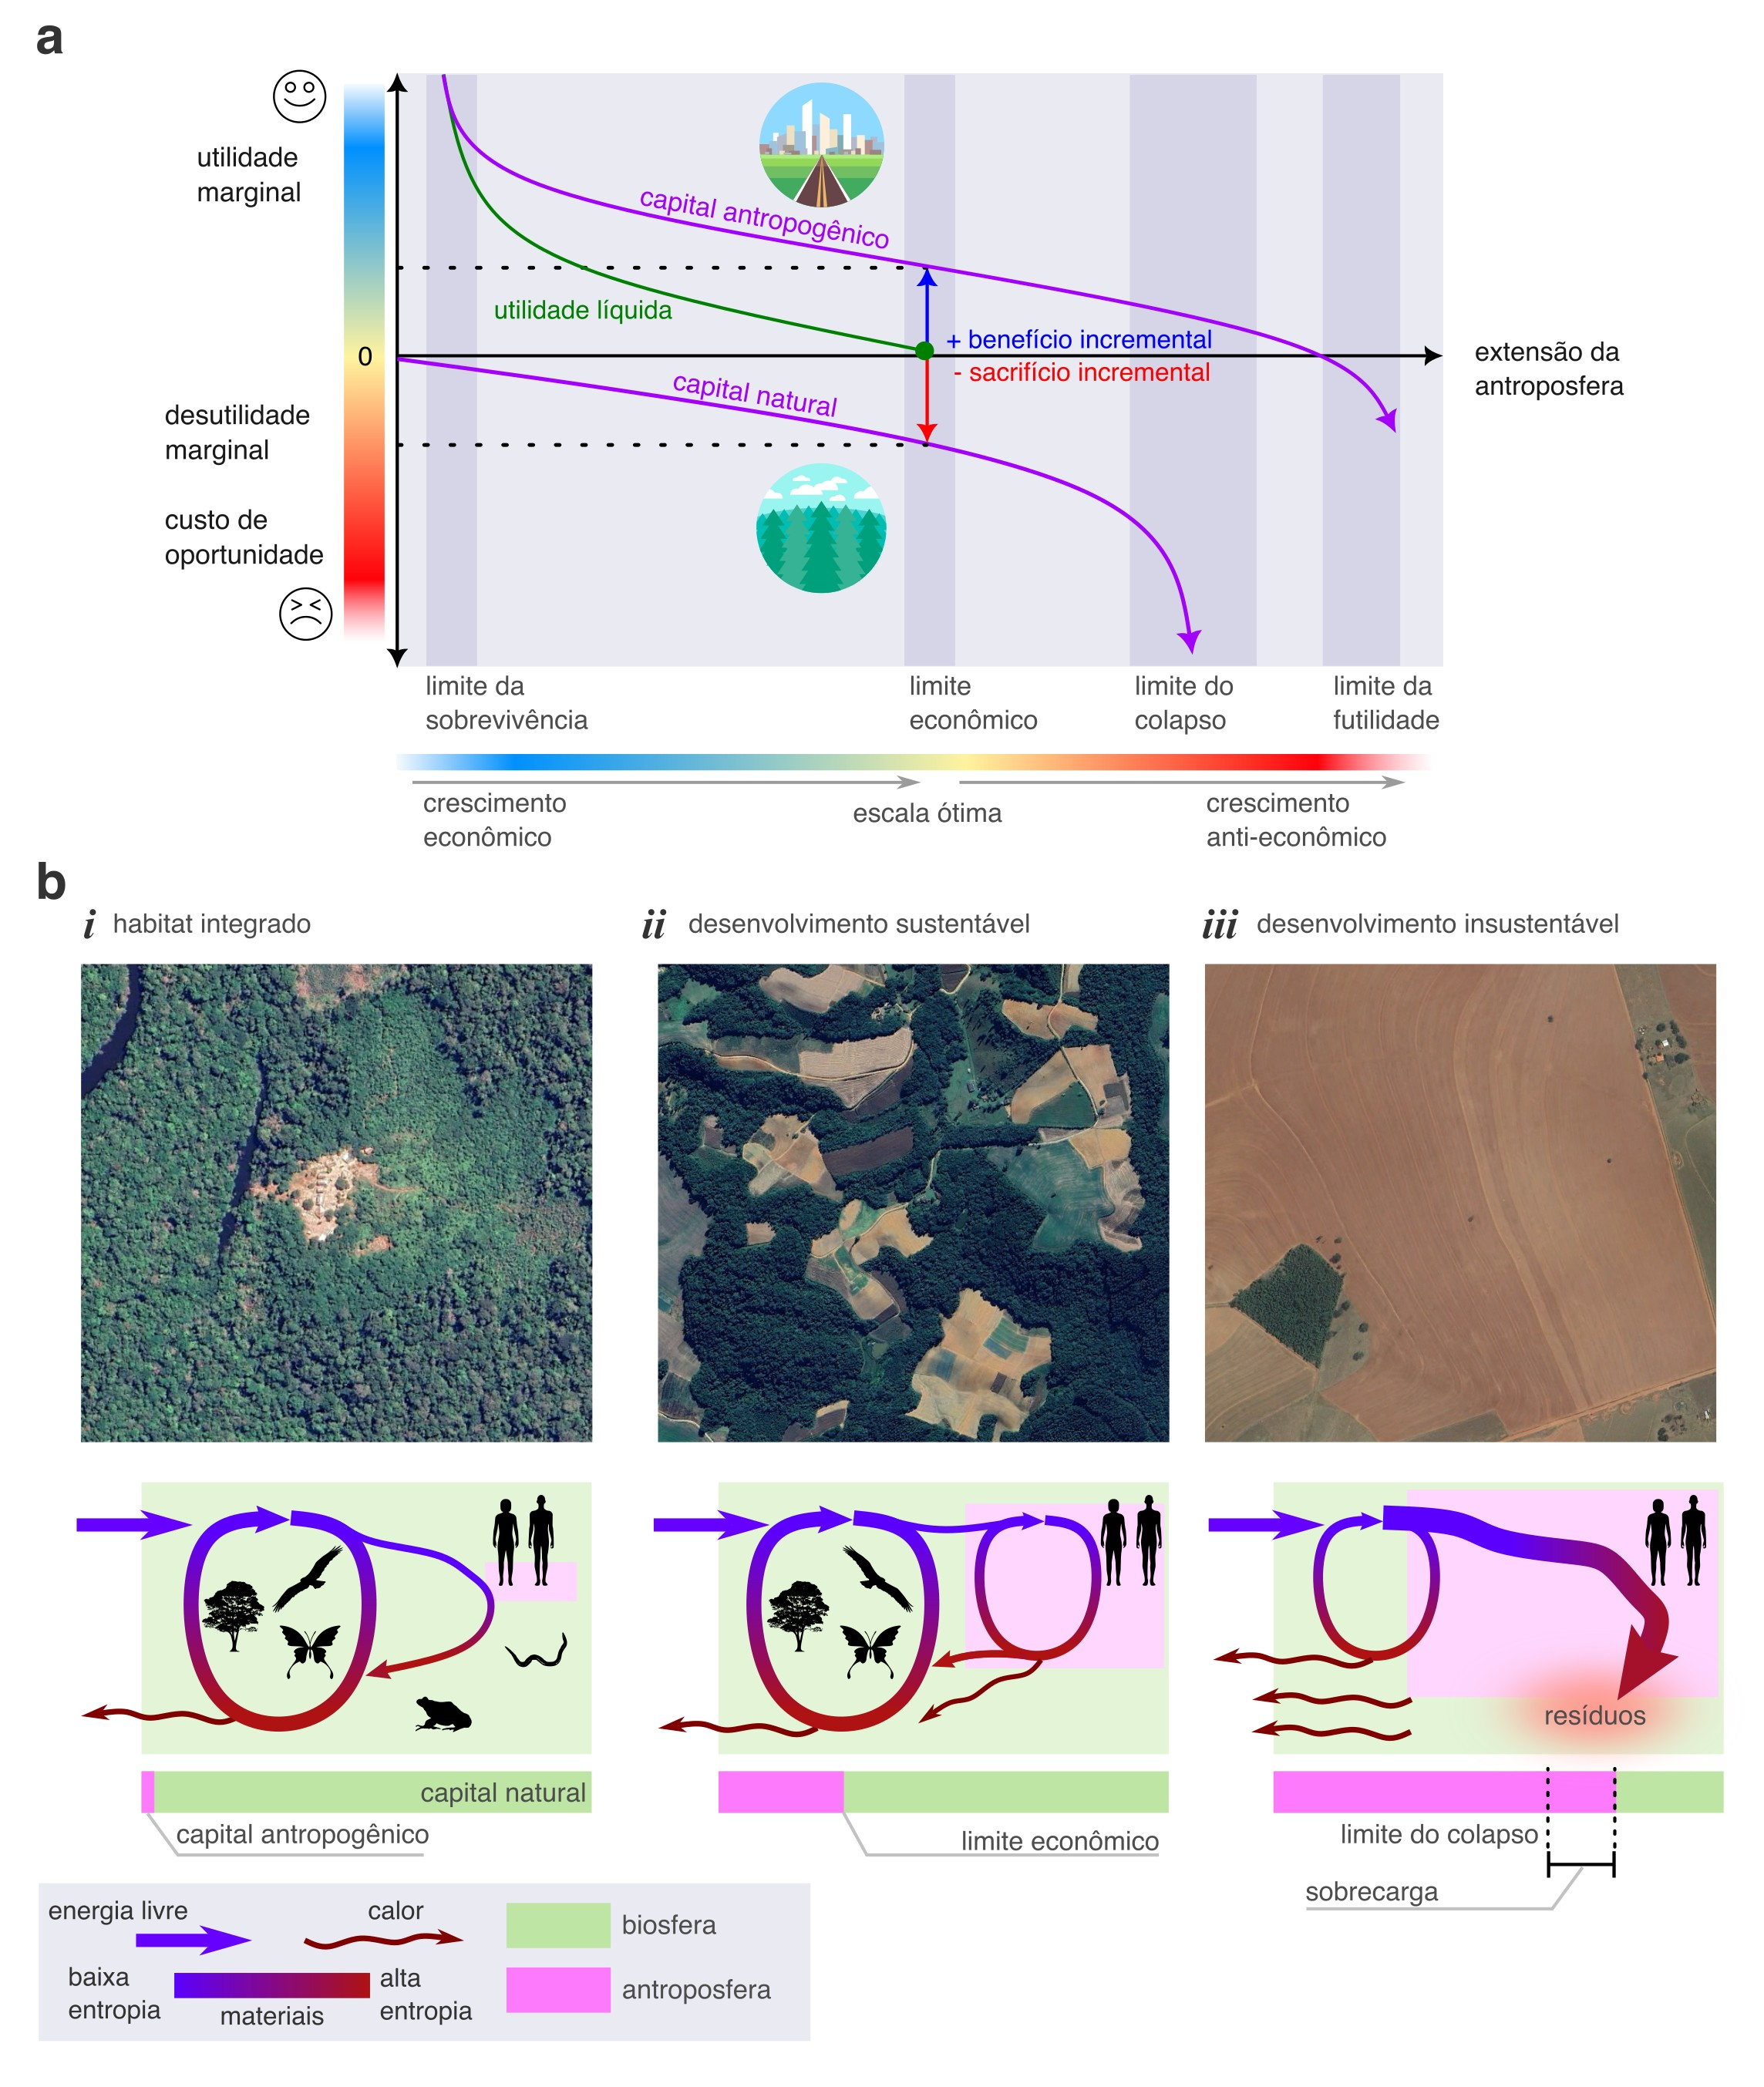
\includegraphics[width=0.98\linewidth]{figs/fig_optscale.jpg}		
\caption[A escala ótima da Antroposfera]
{\textbf{---\;A escala ótima da antroposfera.}
    A principal implicação do modelo ecológico da macroeconomia é que, por ser material, a antroposfera exibe uma extensão econômica sobre a biosfera, ou seja, uma escala ótima. As perguntas de pesquisa do paradigma ecológico orbitam em torno de identificar a escala ótima e outros limites sob diferentes enfoques.
    \;\textbf{a}\;---\;A extensão da antroposfera incorre tanto em uma utilidade marginal decrescente quanto em um custo de oportunidade, ou desutilidade marginal, pelo sacrifício do capital natural pela expansão do capital atropogênico. O limite da sobrevivência, assim, é o habitat minimamente viável que os seres humanos necessitam para metabolizar e se reproduzir. O limite econômico é a escala em que o benefício incremental é equivalente ao sacrifício incremental. Além da escala ótima, a expansão da antroposfera é anti-econômica, pois resulta em uma utilidade marginal líquida negativa. Nessa região há o limite do colapso, que varia conforme a escala de análise e o limite da o limite da futilidade.
    \;\textbf{b}\;---\;A escala ótima pode ser visualizada pelo uso da terra, pela transição gradual entre o habitat integrado de pequenas clareiras abertas (detalhe \textrm{\textit{i}}), passando por um mosaico de fragmentos (detalhe \textrm{\textit{ii}}) até a completa antropização (detalhe \textrm{\textit{iii}}). O desenvolvimento sustentável consiste no tamanho máximo da antroposfera que consegue ainda ser integrada no sistema ecológico, o que exige um fluxo de reciclagem de recursos.
}
\label{fig:eco:escaleopt} 		
\end{figure}

\par Embora a \gls{ecoeco} rejeite as ideias neoclássicas no campo da \gls{macroeon}, ela compartilha vários conceitos fundamentais da \gls{microeon}, como a \gls{marutilteo} e o \gls{ultimategoal} de maximização do \gls{welbeing}. Nesse sentido, Herman Daly \cite{Daly2015a} propõe que, sendo a \gls{antroposf} um sub\gls{system} material da \gls{biosf}, existe uma \textbf{escala ótima} para a \gls{antroposf}, ponto em que o \gls{welbeing} atinge seu máximo, como ilustrado na Figura \ref{fig:eco:escaleopt}. Após o chamado \textbf{\gls{ecolimit}}, o crescimento da \gls{antroposf} se torna anti-econômico, gerando prejuízos crescentes. O conceito de \textbf{\gls{sustdev}} está diretamente ligado a essa ideia, indicando que o crescimento material da economia deve ser balanceado dentro dos limites da \gls{biosf}. Assim, as escolhas econômicas precisam considerar esse equilíbrio, implementando mecanismos e políticas que evitem que a \gls{antroposf} ultrapasse seu ponto ótimo. O programa de pesquisa do \gls{paradigma}, portanto, objetiva investigar quão próximo estamos desse limite. Em um mundo vazio, há espaço para expandir. Já em um mundo lotado, esse limite pode ter sido ultrapassado, exigindo um planejamento que priorize o \textbf{decrescimento} da \gls{antroposf}.

\par O entendimento da escala ótima só é possível ao se generalizar o conceito de \textit{capital} para além da sua concepção convencional. Na visão ecológica, \textbf{\gls{antcap}} consiste nas estruturas materiais e sociais construídas por seres humanos que produzem um fluxo de bens e serviços, resultando em \gls{welbeing}. A definição é vaga e pode ser confundido com a própria \gls{antroposf}. Uma fábrica de motocicletas, por exemplo, consiste em um típico exemplar de capital industrial que produz bens (motocicletas). Uma motocicleta, contudo, pode ser usada para fornecer um serviço de entrega, o que a torna um bem por um lado e um capital por outro. A capacidade de pilotar uma motocicleta faz dos trabalhadores de uma empresa de entregas o seu capital humano. O termo \say{capitalismo}, nesse sentido, consiste na doutrina de acumulação de \gls{antcap}, ou de expansão da \gls{antroposf}. Note-se que, na ótica neoclássica, o capitalismo explicitamente determina o crescimento do capital, mas apenas indiretamente assume que isso irá aumentar o bem-humano, pelo aumento do fluxo de \gls{exchaval}. Como vimos acima, essa doutrina resulta na expansão da \gls{antroposf} sobre a \gls{biosf}, aumentando o \gls{gthoughput}. 

\par Mas além do \gls{antcap}, a visão ecológica também instancia o conceito de \textbf{\gls{natcap}}. A ideia foi articulada inicialmente por Robert Costanza e Herman Daly, em \gls{analogy} ao capital construído \cite{Costanza1992a}. Assim, o \gls{natcap} se define pelas estruturas materiais da própria \gls{biosf} que produzem um fluxo \textit{direto} de bens e serviços, resultando em \gls{welbeing}. Além de bens diretamente utilizáveis, como madeira ou um cardume de peixes, também são considerados serviços, como a polinização, que sustenta a produção de alimentos, a formação de solos férteis, indispensável para a agricultura, e os ciclos biogeoquímicos, como o sequestro de carbono, que regula o clima global. Esses serviços resultam de \textbf{funções ambientais} fundamentais para a vida na Terra, ainda que negligenciados pela abordagem convencional sobre \gls{natrec} \cite{Groot1987a}. Um bom exercício para ilustrar sua importância é imaginar o que seria necessário construir para reproduzir as condições naturais em uma colônia humana em Marte. Sem o suporte do \gls{natcap}, todos os processos essenciais à vida teriam que ser artificialmente replicados, evidenciando a interdependência crítica entre a \gls{antroposf} e a \gls{biosf}.

\par O cerne do conceito de escala ótima, portanto, é reconhecer que a construção de \gls{antcap} exige a desmontagem da infraestrutura existente de \gls{natcap}. Isso resulta obrigatoriamente em um sacrifício de bem-estar provido diretamente pelos recursos e \gls{natserv}. No jargão econômico, existe um \textbf{\gls{opcost}} na expansão da \gls{antroposf}, que é o sacrifício dos recursos e \gls{natserv} providenciados pelo \gls{natcap}. A \gls{marutilteo}, ajuda a ilustrar esse dilema pelo diagrama de \gls{gutility} (Figura \ref{fig:eco:escaleopt}): o \gls{ecolimit} do crescimento do \gls{antcap} ocorre quando a sua \gls{gutility} marginal se iguala à sua \textbf{\gls{desutilmar}}. A \gls{desutilmar} consiste na perda incremental de \gls{gutility} do lado do \gls{natcap}, e consiste exatamente no \gls{opcost}. Esse sacrifício incremental de \gls{gutility} é pequeno em um mundo vazio: uma pequena clareira aberta em uma imensa floresta é praticamente imperceptível em termos de prejuízos, mesmo na \gls{loc-scale} do ecossistema. Na verdade, pode-se conceber que a \gls{antroposf} necessita de um limite mínimo viável, o \textbf{limite da sobrevivência} dos seres humanos na \gls{biosf}. Mas à medida o mundo torna-se lotado, as perdas de \gls{gutility} crescem de forma não linear. Em muitas situações, é possível que um \textbf{\gls{colaplimit}} possa ser superado, quanto processos de degradação praticamente irreversíveis passam a ser desencadeados. A região de sobrecarga é uma situação perigosa, pois atravessar o limite do colapso não implica em uma catástrofe instantânea, devido aos atrasos de propagação dos impactos no sistema ecológico. O diagrama representa a totalidade da \gls{biosf}, mas também pode ser interpretado outras escalas, como em países, bacias, etc, e em relação a processos naturais específicos. Em uma bacia hidrográfica, por exemplo, o \gls{ecolimit} seria uma ocupação do solo e uso da água equilibrada, que preserva diversos outros bens e \gls{natserv}. Um exemplo mais intuitivo é o \gls{system} do clima global: o \gls{ecolimit} seria um nível de poluição por gases de efeito estufa que se compensaria em termos de bem-estar, enquanto que o \gls{colaplimit} representa um nível de poluição em que os processos de mudança climática tornam-se descontrolados, ativando retroações positivas. 

\par O \gls{ecolimit} e o \gls{colaplimit} são em geral inferiores ao \textbf{\gls{futilelimit}}, o nível em que a \gls{gutility} marginal do \gls{antcap} é nula ou mesmo negativa (a situação quando mais recursos trazem diretamente \textit{menos} bem-estar). Isso traz implicações políticas importantes, que confrontam o \textit{status quo} social. A escola econômica Neoclássica tende a ser bem-vista pelas elites sociais, pois ela sugere que basta aumentar o consumo dos recursos para se aumentar o bem-estar coletivo, independentemente das desigualdades relativas entre os consumidores. Com chamada \textbf{promessa da fatia maior} , basta fazer o \say{bolo} crescer para todos que os mais pobres terão amanhã uma fatia maior que hoje – ainda que o fatiamento continue sendo injusto. Mas ao se admitir que existe uma escala ótima para a \gls{antroposf}, vemos que os recursos devem ser consumidos no \gls{ecolimit} para se maximizar o \gls{welbeing}, muito abaixo do \gls{futilelimit}. A única possibilidade viável de alguém consumir recursos acima do \gls{ecolimit} é garantir que outros consumam muito abaixo, um compensando a perda de \gls{natcap} do outro. Mas como esse arranjo desigual não maximiza o bem-estar coletivo, a \gls{ecoeco} postula que, em um mundo material finito, a desigualdade é imoral.  

\subsection{Compreendendo os recursos naturais} \label{subsec:natrec}

\begin{figure}[t!] 
\centering				
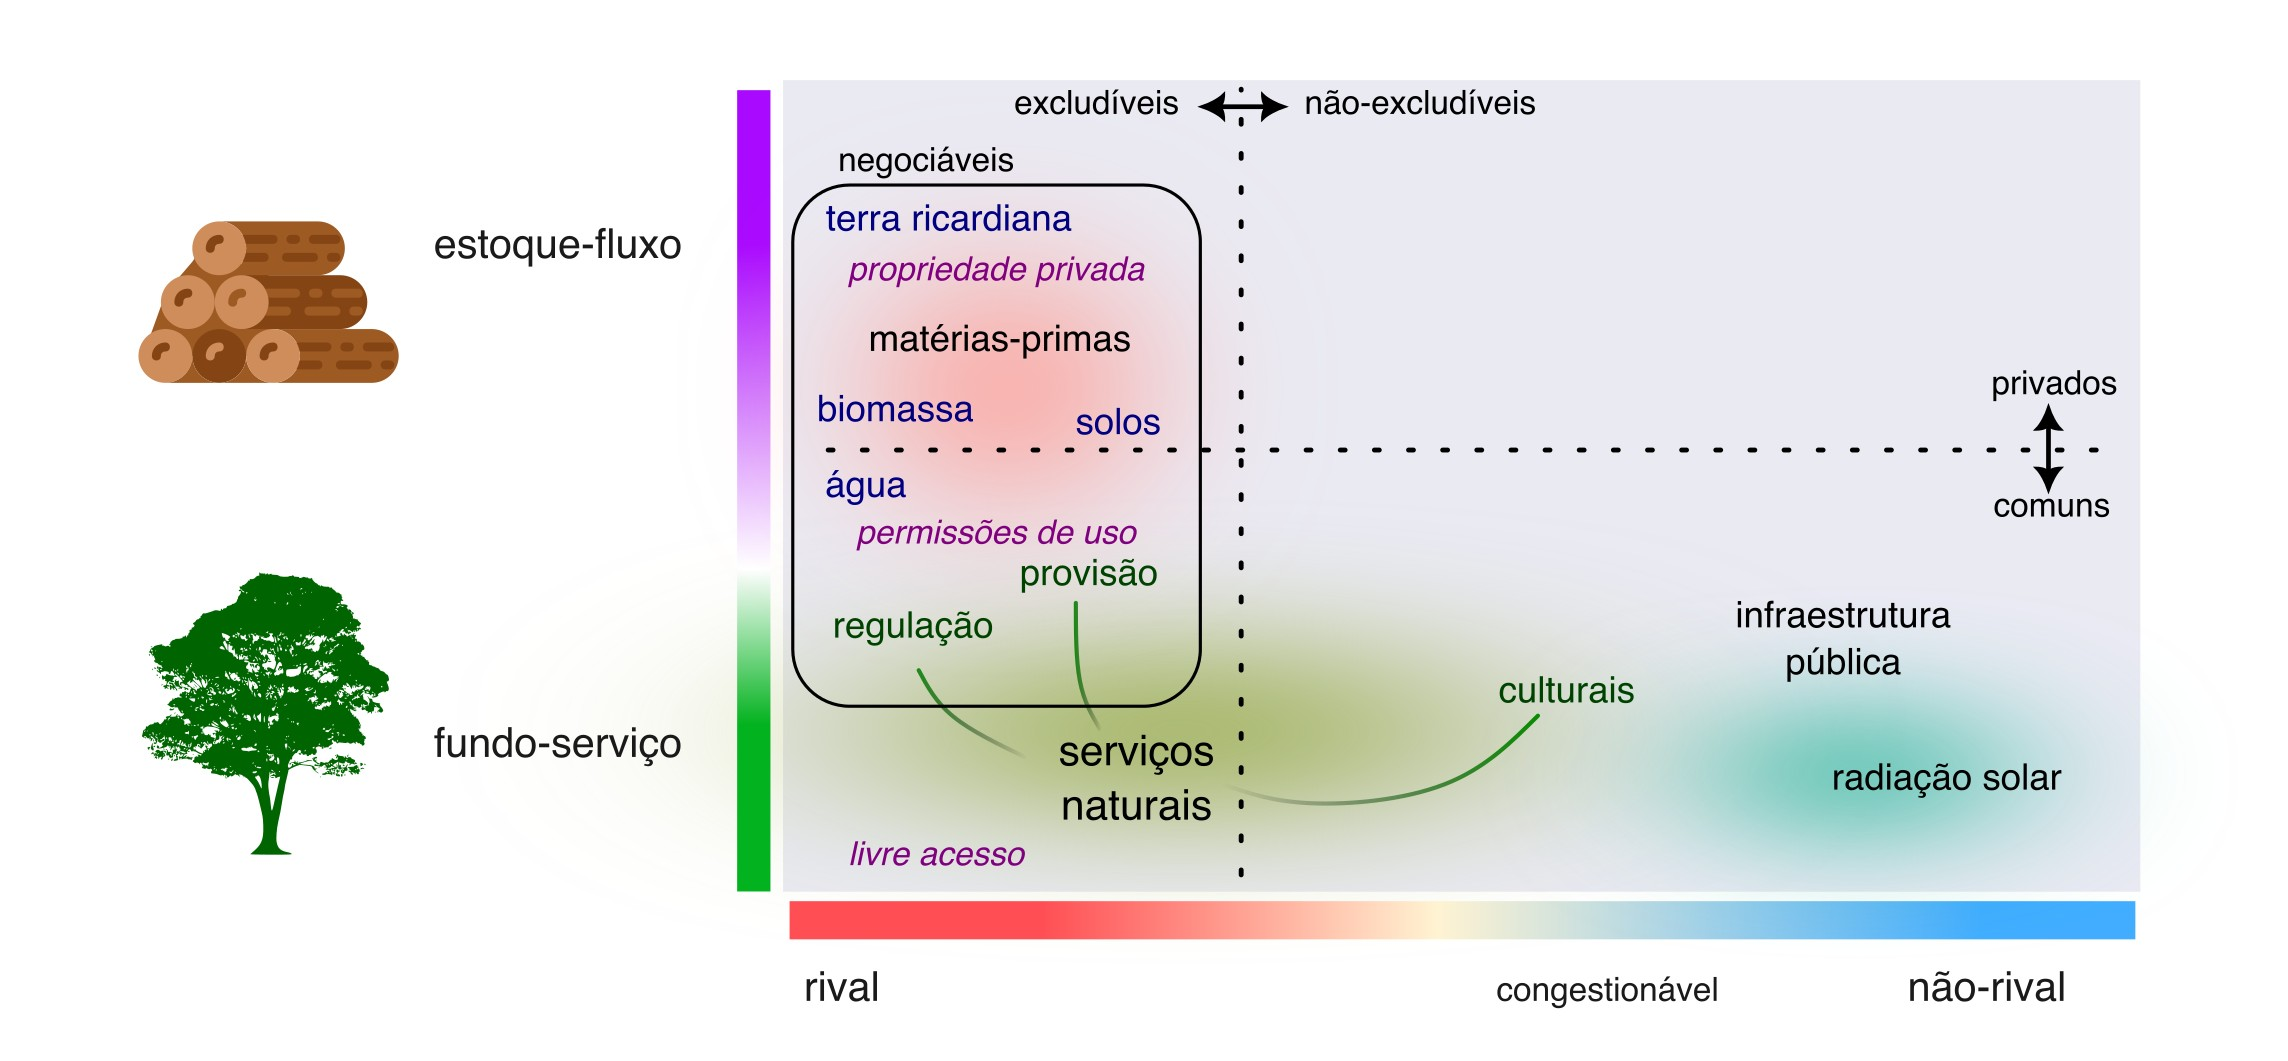
\includegraphics[width=0.98\linewidth]{figs/fig_natrec.jpg}		
\caption[Classificação dos recursos naturais]
{\textbf{---\;Classificação dos \gls{natrec}.}
    O paradigma ecológico organiza os recursos escassos entre tipologias de estoque-fluxo e fundo-serviço. Os recursos de estoque-fluxo oferecem utilidade quando são materialmente transformados durante seu consumo, enquanto que os recursos de fundo-serviço oferecem utilidade sem serem transformados. Os recursos de estoque-fluxo podem ser consumidos a qualquer velocidade, mas esgotam-se subitamente. Os recursos de fundo-serviço só podem ser consumidos a uma velocidade máxima possível e eventualmente podem ficar congestionados. Todos os recursos de estoque-fluxo são rivais por definição, condição que impede múltiplos usuários ao mesmo tempo, e todos os recurso não-rivais, por definição, são fundo-serviços. O serviços naturais, ao contrário das matérias primas, em geral são fundos-serviços rivais, e por isso precisam de alguma forma regulada de exclusividade para evitar o problema do livre acesso.
}
\label{fig:eco:natrec} 		
\end{figure}

\par A classificação dos \textbf{\gls{natrec}} pela \gls{ecoeco} contrasta fortemente com a abordagem da escola Neoclássica. Como a \gls{macroeon} Neoclássica tende a ser uma visão estendida da \gls{microeon}, esse \gls{paradigma} trata os recursos de forma homogênea, reduzindo eles a meros insumos, ou \textbf{fatores de produção}, que contribuem para a maximização de bens e serviços pelo \gls{antcap}. Em geral, os fatores são categorizados em \say{terra} (matérias-primas) e \say{trabalho} (mão de obra), além do próprio capital (máquinas e equipamentos). Na visão Neoclássica, prevalece a ideia de \textbf{capacidade de substituição}, ou seja, a possibilidade de trocar um insumo por outro quando este estiver escasso, o que gera uma relativa insensibilidade ao esgotamento dos recursos utilizados. Por não reconhecer a existência de \gls{natcap}, o esgotamento de matérias-primas não é considerado um problema de base, desde que possam ser substituídas com o advento de inovações tecnológicas. 

\par Não obstante, Herman Daly articula uma distinção crítica entre \textbf{\gls{recstflow}}, que podem ser consumidos em qualquer ritmo, e os \textbf{\gls{fundserv}}, cuja produtividade é limitada no tempo e que não podem ser facilmente substituídos \cite{daly2011}. O \gls{natcap} pode ser de um tipo ou de outro. Mas também pode ser ambos, como no caso das florestas. As florestas são um estoque-fluxo de madeira, uma matéria-prima. Mas também são um fundo-serviço de diversos \textbf{\gls{natserv}} (ver Figura \ref{fig:eco:natrec}). Com isso, o \gls{scale_problem} ótima se faz evidente: o \gls{econbenefit} de desmontar uma floresta vem junto com o \gls{opcost} dos \gls{natserv} sacrificados. Mas como as florestas são um \gls{system} que se regenera com energia do sol, é possível encontrar um fluxo sustentável de obtenção de madeira sem abrir completamente mão dos \gls{natserv}. Essa classificação ressalta a necessidade de estratégias que levem em consideração os limites e a \textbf{insubstituibilidade} de certos recursos, oferecendo uma estrutura mais adequada para se desenhar políticas de \gls{sustdev}.

\par Os \gls{recstflow} são aqueles que são materialmente transformados durante o processo produtivo, ou seja, tornam-se parte do produto final. No contexto do \gls{natcap}, esses recursos são classificados como \textbf{\gls{recrenew}} e \textbf{\gls{recnotrenew}}. Um exemplo claro é o petróleo, que é refinado em combustível, ou as árvores, que são convertidas em tábuas e papel. Quando disponíveis, esses recursos podem ser consumidos a praticamente qualquer ritmo. Por exemplo, grandes quantidades de petróleo podem ser extraídas rapidamente, desde que existam poços suficientes e refinarias em operação. De forma semelhante, uma floresta pode ser desmatada em poucos dias, se houver máquinas e trabalhadores suficientes. Esses recursos também podem ser estocados para uso futuro; matérias-primas como grãos, combustíveis e minerais podem ser armazenados em depósitos, permitindo um gerenciamento flexível ao longo do tempo. Similarmente, talhões de florestas podem ser preservados para corte em ocasiões futuras. 

\par Quando consumidos a uma velocidade maior que a \textbf{\gls{carycap}}, os \gls{recstflow} se esgotam subitamente. Como o petróleo leva milhões de anos para se formar naturalmente, ele é considerado um recurso não renovável, assim como a maioria dos \textbf{\gls{recmineral}}. Já as florestas, quando manejadas adequadamente, podem se regenerar em um período razoavelmente curto de tempo, o que torna a madeira das árvores um recurso renovável, assim como a maioria dos \textbf{\gls{recbio}}. A água, apesar de ser um \textbf{\gls{recabio}}, também é um recurso renovável, pois o \gls{hydro_cicle} atua constantemente, eventualmente regenerando os níveis dos rios e lagos.  Contudo, uma vez utilizados, esses recursos são destruídos e não podem ser recuperados em sua forma original. Em certos casos, os resíduos gerados podem ser reutilizados em outros processos ou reciclados. A identificação de \textbf{\gls{recreus}} e \textbf{\gls{recreci}} consiste em uma estratégia essencial para a sustentabilidade, pois reduz o \gls{gthoughput} na \gls{antroposf}. Ainda assim, é preciso lembrar que esses processos não reduzem a necessidade de importar energia livre para a realização de trabalho.

\par Por outro lado, \gls{fundserv} são aqueles que participam do processo produtivo \textit{sem} se transformarem fisicamente no produto final. Eles fornecem os meios e serviços essenciais para o processo produtivo, mas não se esgotam de imediado. A destruição desses recursos ocorre pelo desgaste ou \textbf{\gls{deprec}} ao longo do tempo, pela ação da \gls{secondlaw}. No caso do \gls{antcap}, infraestruturas como rodovias, sistemas energéticos, redes de comunicação, além de máquinas e mão de obra, são exemplos desses recursos. Eles não se tornam parte do produto final; uma máquina de costura, por exemplo, participa da fabricação de roupas, mas não se incorpora no produto. Em contraste com os \gls{recstflow}, os \gls{fundserv} têm uma capacidade limitada de produção por unidade de tempo. Uma máquina ou um trabalhador pode produzir apenas uma quantidade finita de produtos em um determinado período, independentemente da quantidade de matéria-prima disponível. Além disso, esses serviços não podem ser estocados. Se uma fábrica fica inativa por uma semana, a capacidade produtiva dessa semana é perdida e não pode ser recuperada posteriormente. Com o tempo, esses recursos se desgastam; uma máquina, por exemplo, enferruja e precisa de manutenção, e os trabalhadores necessitam de descanso e capacitação contínua para manter a sua produtividade. Por isso, esses recursos não existem de forma estática, mas também participam no \gls{gthoughput}, consumindo energia livre e materiais de baixa entropia.

\par Ao contrário do \gls{antcap}, que depende de manutenção contínua por intervenções humanas, o \gls{natcap} possui intrínsecos mecanismos de \textbf{\gls{selforg}}. Os ciclos biogeoquímicos, por exemplo, são impulsionados por fontes de energia livres como a radiação solar e o calor do núcleo terrestre, tornando a \gls{biosf} um \gls{system} auto-organizado que sustenta a vida e regula os fluxos de materiais e energia. Como veremos adiante com mais detalhes, os \gls{natserv} são os \gls{fundserv} que obtemos diretamente desse \gls{system} autorregulado. Esses serviços podem ser categorizados em três grandes grupos: os \textbf{\gls{natservprov}}, que abrangem a capacidade da \gls{biosf} de fornecer e regenerar \gls{recstflow}, como alimentos, água e matérias-primas; os \textbf{\gls{natservreg}}, que controlam processos vitais como o ciclo da água, a regulação do clima e a polinização, equilibrando e organizando os fluxos materiais dentro da \gls{biosf}; e os \textbf{\gls{natservcult}}, que se referem ao bem-estar imaterial proporcionado pela interação humana direta com o ambiente natural, seja através de atividades recreativas, científicas, religiosas ou espirituais. Exemplos concretos desses serviços incluem a capacidade de florestas tropicais de sequestrar carbono da atmosfera, regulando o clima global, ou os recifes de corais, que não só fornecem habitats para uma vasta biodiversidade marinha, mas também servem como barreiras naturais contra tempestades costeiras. Da mesma forma, a interação com paisagens naturais, como parques nacionais, promove a saúde mental e o \gls{welbeing}, exemplificando a dimensão cultural desses serviços.

\subsection{O problema do livre acesso} \label{subsec:tragedy}

\begin{figure}[t!] 
\centering				
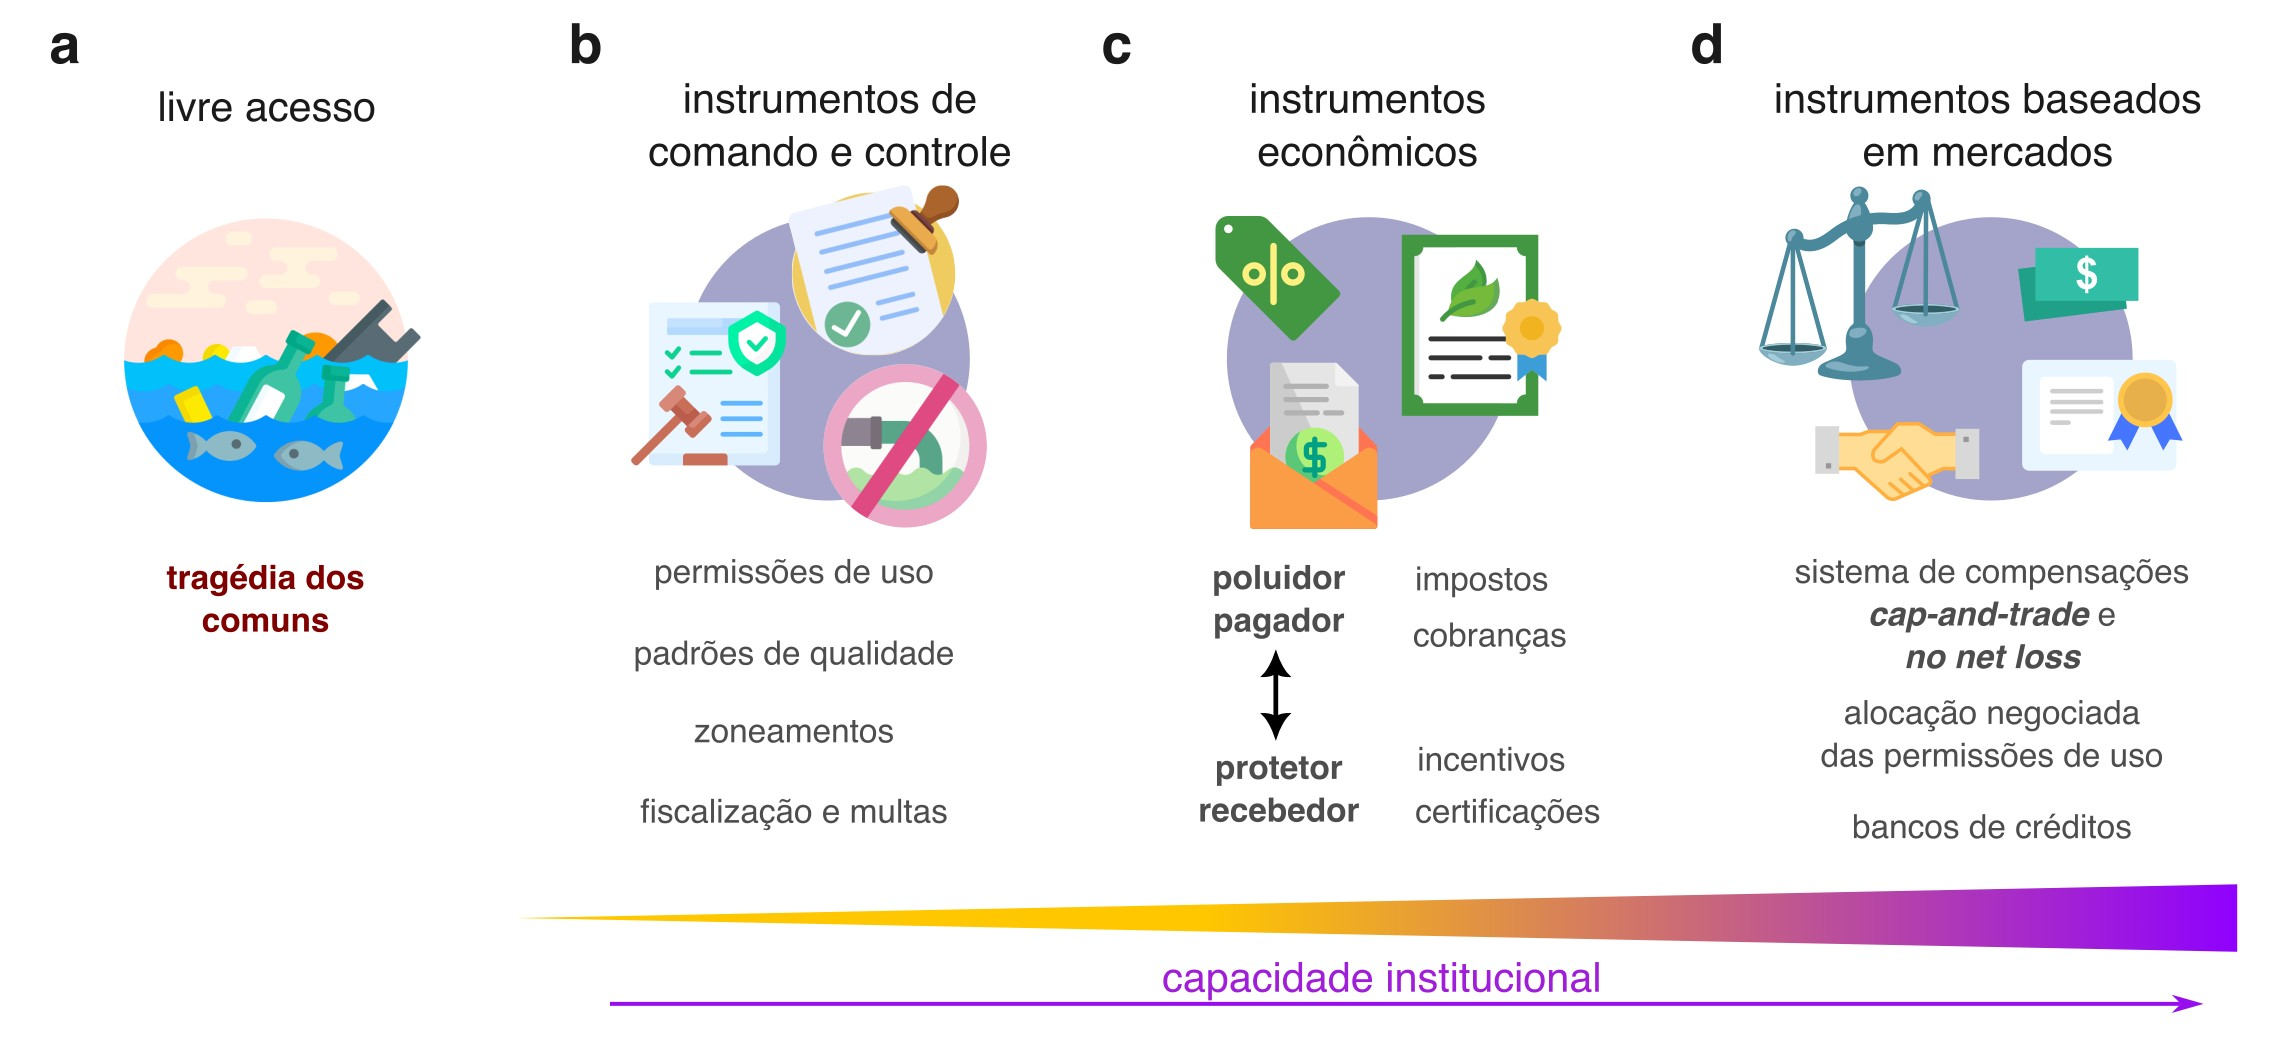
\includegraphics[width=0.98\linewidth]{figs/fig_opensacc.jpg}		
\caption[Soluções para o problema do livre acesso]
{\textbf{---\;Soluções para o \gls{probfreeacc}.}
    O problema do livre acesso surge diante de recursos comuns, que não possuem exclusividade instituída. A solução passa por camadas incrementais de instrumentos de gestão, que exigem maior capacidade institucional do Estado.
    \;\textbf{a}\;---\;Sem regulações sobre o uso dos recursos comuns, a ação individual gera uma corrida desenfreada para utilizar os serviços-naturais e matérias-primas, produzindo a tragédia dos comuns -- um colapso ambiental.
    \;\textbf{b}\;---\;Instrumentos de comando e controle são a primeira camada de gestão, definindo regras gerais aplicadas por força de lei sobre os agentes econômicos, como permissões de uso, padrões de qualidade, zoneamentos e penalidades em caso de infrações. 
    \;\textbf{c}\;---\;Instrumentos econômicos formam a segunda camada de gestão, induzindo os agentes econômicos a mudarem seu comportamento para além das regras gerais obrigatórias. No caso, podem tanto ser articulados o princípio do poluidor-pagador, com impostos e cobranças, quanto o princípio do protetor-recebedor, com incentivos e certificações. 
    \;\textbf{d}\;---\;Instrumentos baseados em mercados formam uma terceira camada de gestão, criando um espaço de negociações das permissões de uso para os agentes econômicos encontrarem arranjos otimizados por conta própria. Nesse instrumento, geralmente são definidos sistemas de compensações, que criam um mercado de créditos e débitos, como \textit{cap-and-trade} e \textit{no net loss}. Bancos são necessários para facilitar e reduzir o custo de transação. 
}
\label{fig:eco:tragedy} 		
\end{figure}

\par Desenhar políticas de alocação de recursos para manter a \gls{antroposf} no seu \gls{ecolimit} passa invariavelmente por endereçar o \textbf{\gls{probfreeacc}}. Esse problema foi articulado no artigo \textit{A tragédia dos comuns} pelo ecólogo Garret Hardin (1968) \cite{Hardin1968a}. Nesse artigo, Hardin argumenta que os problemas ambientais, como o sobreuso da terra e a poluição da água, são consequência do livre acesso de bens e serviços que são de uso comum, ou \textbf{\gls{reccom}}\footnote{Esse termo refere-se tanto ao \gls{natcap} quanto ao \gls{antcap}.}. Como os indivíduos e empresas agem para maximizar apenas o seu bem-estar individual, o livre acesso acaba criando uma corrida desenfreada para aproveitar o recurso, que acaba sendo congestionado ou esgotado. Configura-se uma tragédia, portanto, pois a ação supostamente racional dos indivíduos termina por ser um movimento irracional do coletivo. Hardin reconhece, com isso, que fazer do recurso público um bem análogo a recursos privados pode ser uma solução interessante, mas que não se aplica em todos os casos:

\begin{adjustwidth}{100pt}{0pt}
\medskip
\small A tragédia dos comuns, entendida como uma cesta de alimentos, é evitada pela \gls{privprop}, ou algo formalmente semelhante. Mas o ar e as águas ao nosso redor não podem ser facilmente cercados, e assim a tragédia dos comuns, entendida como uma fossa séptica, deve ser evitada por outros meios, através de leis coercitivas ou dispositivos de taxação que tornem mais barato para o poluidor tratar seus poluentes do que descartá-los sem tratamento. Não avançamos tanto na solução desse problema quanto no primeiro. De fato, nosso conceito particular de \gls{privprop}, que nos impede de esgotar os recursos da Terra, favorece a poluição. O proprietário de uma fábrica na margem de um rio — cuja propriedade se estende até o meio do rio — muitas vezes tem dificuldade em entender por que não é seu direito natural poluir as águas que passam por sua porta. A lei, sempre desatualizada, exige uma adaptação elaborada para se ajustar a este aspecto recentemente percebido dos bens comuns.\footnote{
Tradução livre de: \textit{The tragedy of the commons as a food basket is averted by private property, or something formally like it. But the air and waters surrounding us cannot readily be fenced, and so the tragedy of the commons as a cesspool must be prevented by different means, through coercive laws or taxing devices that make it cheaper for the polluter to treat their pollutants than to discharge them untreated. We have not progressed as far with the solution to this problem as we have with the first. Indeed, our particular concept of private property, which deters us from exhausting the positive resources of the earth, favors pollution. The owner of a factory on the bank of a stream—whose property extends to the middle of the stream—often has difficulty seeing why it is not their natural right to muddy the waters flowing past their door. The law, always behind the times, requires elaborate stitching and fitting to adapt it to this newly perceived aspect of the commons.}
} -- Garret Hardin (1968, p. 1245) \cite{Barnes1939}.
\medskip
\end{adjustwidth}

\noindent O problema da poluição da água e do ar pode ser resolvido ao impor que os poluidores assumam total responsabilidade por seus resíduos. Um conceito central da \gls{microeon} Neoclássica, nesse sentido, é o de \textbf{\gls{external}}, que pode ser positiva ou negativa. Externalidade refere-se ao impacto das ações de um agente econômico sobre o bem-estar de outros \cite{Mankiw2002a}. No exemplo de Hardin, em que uma fábrica polui o ar e a água, devem ser criados mecanismos regulatórios para evitar a perda de bem-estar coletivo (a \gls{external} negativa), obrigando a fábrica a gerir seus resíduos, mesmo que isso seja mais oneroso. Nesse contexto, a \gls{ecoeco} oferece uma interpretação mais ampla do \gls{probfreeacc} e das externalidades em comparação com a \gls{microeon} Neoclássica. O conceito de \gls{external} negativa, segundo essa visão, está relacionado ao \gls{opcost} da expansão da \gls{antroposf} sobre a \gls{biosf}. A transformação de um rio em um canal de efluentes gera uma série de externalidades negativas precisamente pela perda de \gls{natcap} -- os recursos e serviços diretamente fornecidos pelo rio, desde o fornecimento de água potável até atividades culturais. 

\par Aqui, os conceitos de \textbf{\gls{rivalty}} e \textbf{\gls{exclusvty}}, também da \gls{microeon}, são relevantes para se conceber políticas de alocação adequadas. Os \textbf{\gls{recrival}} exibem uma característica intrínseca que impede seu uso por múltiplos agentes econômicos ao mesmo tempo. A interpretação disso é bastante intuitiva: se uma padaria consome a farinha de um silo, ela automaticamente impede outra padaria de fazer o mesmo; se um barco de pesca captura um cardume, ele automaticamente impede outro barco de fazer o mesmo; se um agricultor planta milho em uma gleba de terra, ele impede outro de criar ovelhas na mesma gleba. Todos os recursos rivais são \textbf{excludíveis}, mas não necessariamente exclusivos. Isso ocorre porque os \textbf{\gls{recexclu}} exigem uma garantia social de uso reservado por um dado agente econômico, mas isso nem sempre existe. A \gls{exclusvty} faz surgir mercados, pois torna os \gls{recrival} em \textbf{\gls{rectrad}}, encorajando os agentes econômicos a alocar recursos entre si pelo seu \gls{exchaval}. A garantia de \gls{exclusvty} se manifesta, em sua essência, pela \textit{dissuasão} entre os agentes econômicos. Em sociedades de pequena escala, como famílias e clãs, essa dissuasão pode ocorrer através de acordos tácitos. Já em sociedades maiores, em que desconhecidos interagem, o Estado tende a garantir o direito de uso por meio do monopólio da força e da difusão de normas culturais de convívio. O direito à \textbf{\gls{privprop}} é uma instituição criada pelo Estado para conferir ao proprietário, mediante documento oficial, o uso exclusivo de um recurso rival. Para negociar o recurso, é preciso também negociar o documento oficial do Estado que institui a \gls{exclusvty}. A diferença entre a \gls{privprop} e uma concessão pública está no fato de que a propriedade é vitalícia e hereditária, mas ambos são garantias de exclusividade fornecidas pelo Estado. Em sociedades grandes, mas com Estados fracos, a \gls{exclusvty} também pode ocorrer, mas frequentemente exige maior investimento em mecanismos privados de dissuasão, como cercas, armas e emprego de mercenários.

\par Todos os \gls{recstflow} são rivais e todos os \textbf{\gls{recnonrival}} são fundos-serviços. Como os \gls{recstflow} são destruídos durante o seu uso, isso os torna inerentemente rivais -- o mesmo carvão queimado por uma usina não pode ser queimado por outra. Já os \gls{recnonrival}, por definição, são aqueles que podem ser consumidos por mais de um agente econômico \textit{ao mesmo tempo}. Logicamente, portanto, esses recursos não podem ser \gls{recstflow}. São \gls{reccom}, de uso geral, acessíveis por todos ao mesmo tempo e que não são esgotáveis nem acumuláveis. Um recurso não-rival típico é a radiação solar, um fluxo de energia livre que é distribuída de maneira relativamente homogênea. Se uma planta realiza a fotossíntese com a luz do sol, ela não impede automaticamente outras plantas de também realizar a fotossíntese ao mesmo tempo. Outro exemplo típico são as vias de transporte, como ruas e estradas. Se um automóvel trafega por uma rua, ele não impede outro automóvel de trafegar ao mesmo tempo. Da mesma forma, a beleza cênica de parques e praias oferece bem-estar aos seus usuários indistintamente.

\par O \gls{probfreeacc} pode ser separado entre a sua forma branda, que envolve \gls{recnonrival}, e sua forma severa, que envolve \gls{recrival}. Os \gls{recnonrival}, sendo necessariamente \gls{fundserv}, são considerados \textbf{\gls{reccongest}}, pois podem ser consumidos até o limite de sua taxa de provisão. O congestionamento, como uma forma branda do \gls{probfreeacc}, ocorre quando o recurso não é destruído nem degradado durante o uso, mas impõe um número máximo de usuários. Exemplos típicos ocorrem quando edifícios muito altos bloqueiam a iluminação solar para edifícios menores; quando o \gls{system} viário torna-se superlotado com a quantidade de automóveis; ou quando os parques e praias são tomadas por multidões em busca de lazer. Em todos esse casos, os serviços oferecidos pelos recursos perdem eventualmente seu \gls{useval}, em função do livre acesso. Nesse caso, a solução do problema passa inexoravelmente por \textbf{\gls{instrcc}}, imposições coercitivas do Estado articuladas pela ação de autoridades reguladoras, além de estratégias auxiliares, como reforçar as normas culturais. 

\par A versão severa do \gls{probfreeacc} ocorre no contexto de \gls{reccom} rivais, pois o seu consumo descontrolado não produz apenas um congestionamento, mas pode levar a um colapso ambiental -- a \say{tragédia dos comuns} de Hardin, mencionada acima. Isso é evidente no caso de \gls{reccom} do tipo estoque-fluxo, como quando a água dos rios é usada como insumo de processos produtivos. Nessa situação, o livre acesso potencialmente leva os agentes econômicos a utilizarem toda a água disponível nos mananciais, produzindo um cenário de escassez e todas as \gls{external} negativas associadas. Mas a água dos rios também pode ser usada como um fundo-serviço público, como no caso da poluição. Aqui, a capacidade de diluição e autodepuração de resíduos de um curso d'água é um exemplo de um fundo-serviço \textit{que também é rival}. O rio em si não é transformado em nenhum novo produto, mas o serviço natural de regulação da qualidade ambiental é progressivamente degradado à medida que é utilizado. Quando uma indústria lança resíduos no rio, a capacidade de diluição original é consumida, impossibilitando o uso simultâneo desse serviço pela próxima indústria, rio abaixo. 

\par A solução para o problema grave do livre acesso também envolve a possibilidade de se implementar alguma forma de \gls{exclusvty} através da emissão oficial de \textbf{\gls{usepermits}} para os agentes econômicos \cite{Schlager1992}. As permissões de uso de \gls{reccom} não são \gls{privprop}, o que implica um direito de uso vitalício e hereditário, se aproximando mais de concessões públicas, que são periodicamente revisadas e renovadas por instituições reguladoras. No caso da água, a permissão oficial para captação, por exemplo, estabelece a \gls{exclusvty} de uso dentro de limites pré-definidos, compatíveis com a disponibilidade natural dos mananciais. Similarmente, permissões oficiais de lançamento de efluentes visam regular o uso da capacidade de diluição, limitando novamente os usuários. Assim, podem-se desenhar políticas de alocação que variam desde \gls{instrcc} convencionais, que estabelecem as regras gerais, até \textbf{\gls{instecon}} que não apenas aplicam punições para externalidades negativas (\textbf{princípio do poluidor-pagador}[todo:gls]), mas também oferecem incentivos para os usuários que geram externalidades positivas (\textbf{princípio do protetor-recebedor}) [todo:gls]. Um avanço nesse sentido são os \textbf{\gls{instrmarkt}}, ou políticas de \textit{cap-and-trade} \cite{Borghesi2013}. Nesse tipo de regulação, os recursos mantêm sua natureza pública, mas a \gls{usepermits} define-se por cotas exclusivas, que podem ser livremente negociadas entre os agentes econômicos. Um exemplo clássico desse instrumento é o mercado de carbono, onde agentes com créditos (carbono sequestrado) negociam com agentes com débito (carbono emitido), mantendo o \gls{system} em uma condição neutra \cite{Mazaheri2022}.

\par Aqui, cabe ressaltar que o desenvolvimento de \gls{instecon} e \gls{instrmarkt} demandam uma \textbf{\gls{insticap}} da parte do Estado \textit{maior} do que o simples comando e controle. Isso ocorre em razão dessas políticas de gestão não serem exatamente substitutas umas das outras, sendo na realidade estratégias incrementalmente mais complexas. O comando e controle, por conta própria, não é capaz de interferir sobre os agentes econômicos para além de garantir o cumprimento de \textit{regrais gerais}, como padrões de qualidade, zoneamento, etc. Se os \gls{instrcc} avançam além de regras gerais, os agentes econômicos deixam de existir \textit{por definição}, tornando-se extensões do próprio Estado. Em sociedades que toleram a existência de múltiplos agentes econômicos, portanto, o Estado precisa de um aparato institucional extra para operacionalizar o limite econômico sem tomar as decisões pelos agentes. Os \gls{instecon}, nessa linha, visam incentivar mudanças de comportamento que não são obrigatórias, mas \textit{desejáveis}. Os \gls{instrmarkt} vão além, com maior potencial de maximizar o \gls{econbenefit} total, pois as negociações tendem a encontrar uma solução otimizada de alocação, dentro dos limites impostos previamente. No exemplo da poluição, o aparato de regulação e fiscalização compõe uma base de comando e controle que não pode ser abandonada, que define padrões de lançamento, monitora e aplica penalidades. Sobreposto ao arcabouço de comando e controle, é possível criar um sistema de incentivos para reduzir ainda mais o uso do serviço natural, como estimular o reúso de água. Porém, manter e atualizar um \textbf{banco de créditos} exige uma maior carga administrativa do que apenas o aparato de fiscalização anterior. Por fim, um mercado de permissões de lançamento pode ser implementado, mas não sem o advento de uma instituição que o viabilize e regule sua dinâmica, reduzindo o \textbf{\gls{costtransac}} embutido em negociar as permissões.

\section{Serviços naturais} \label{chap:ecoeco:natserv}

\begin{figure}[t!] 
\centering				
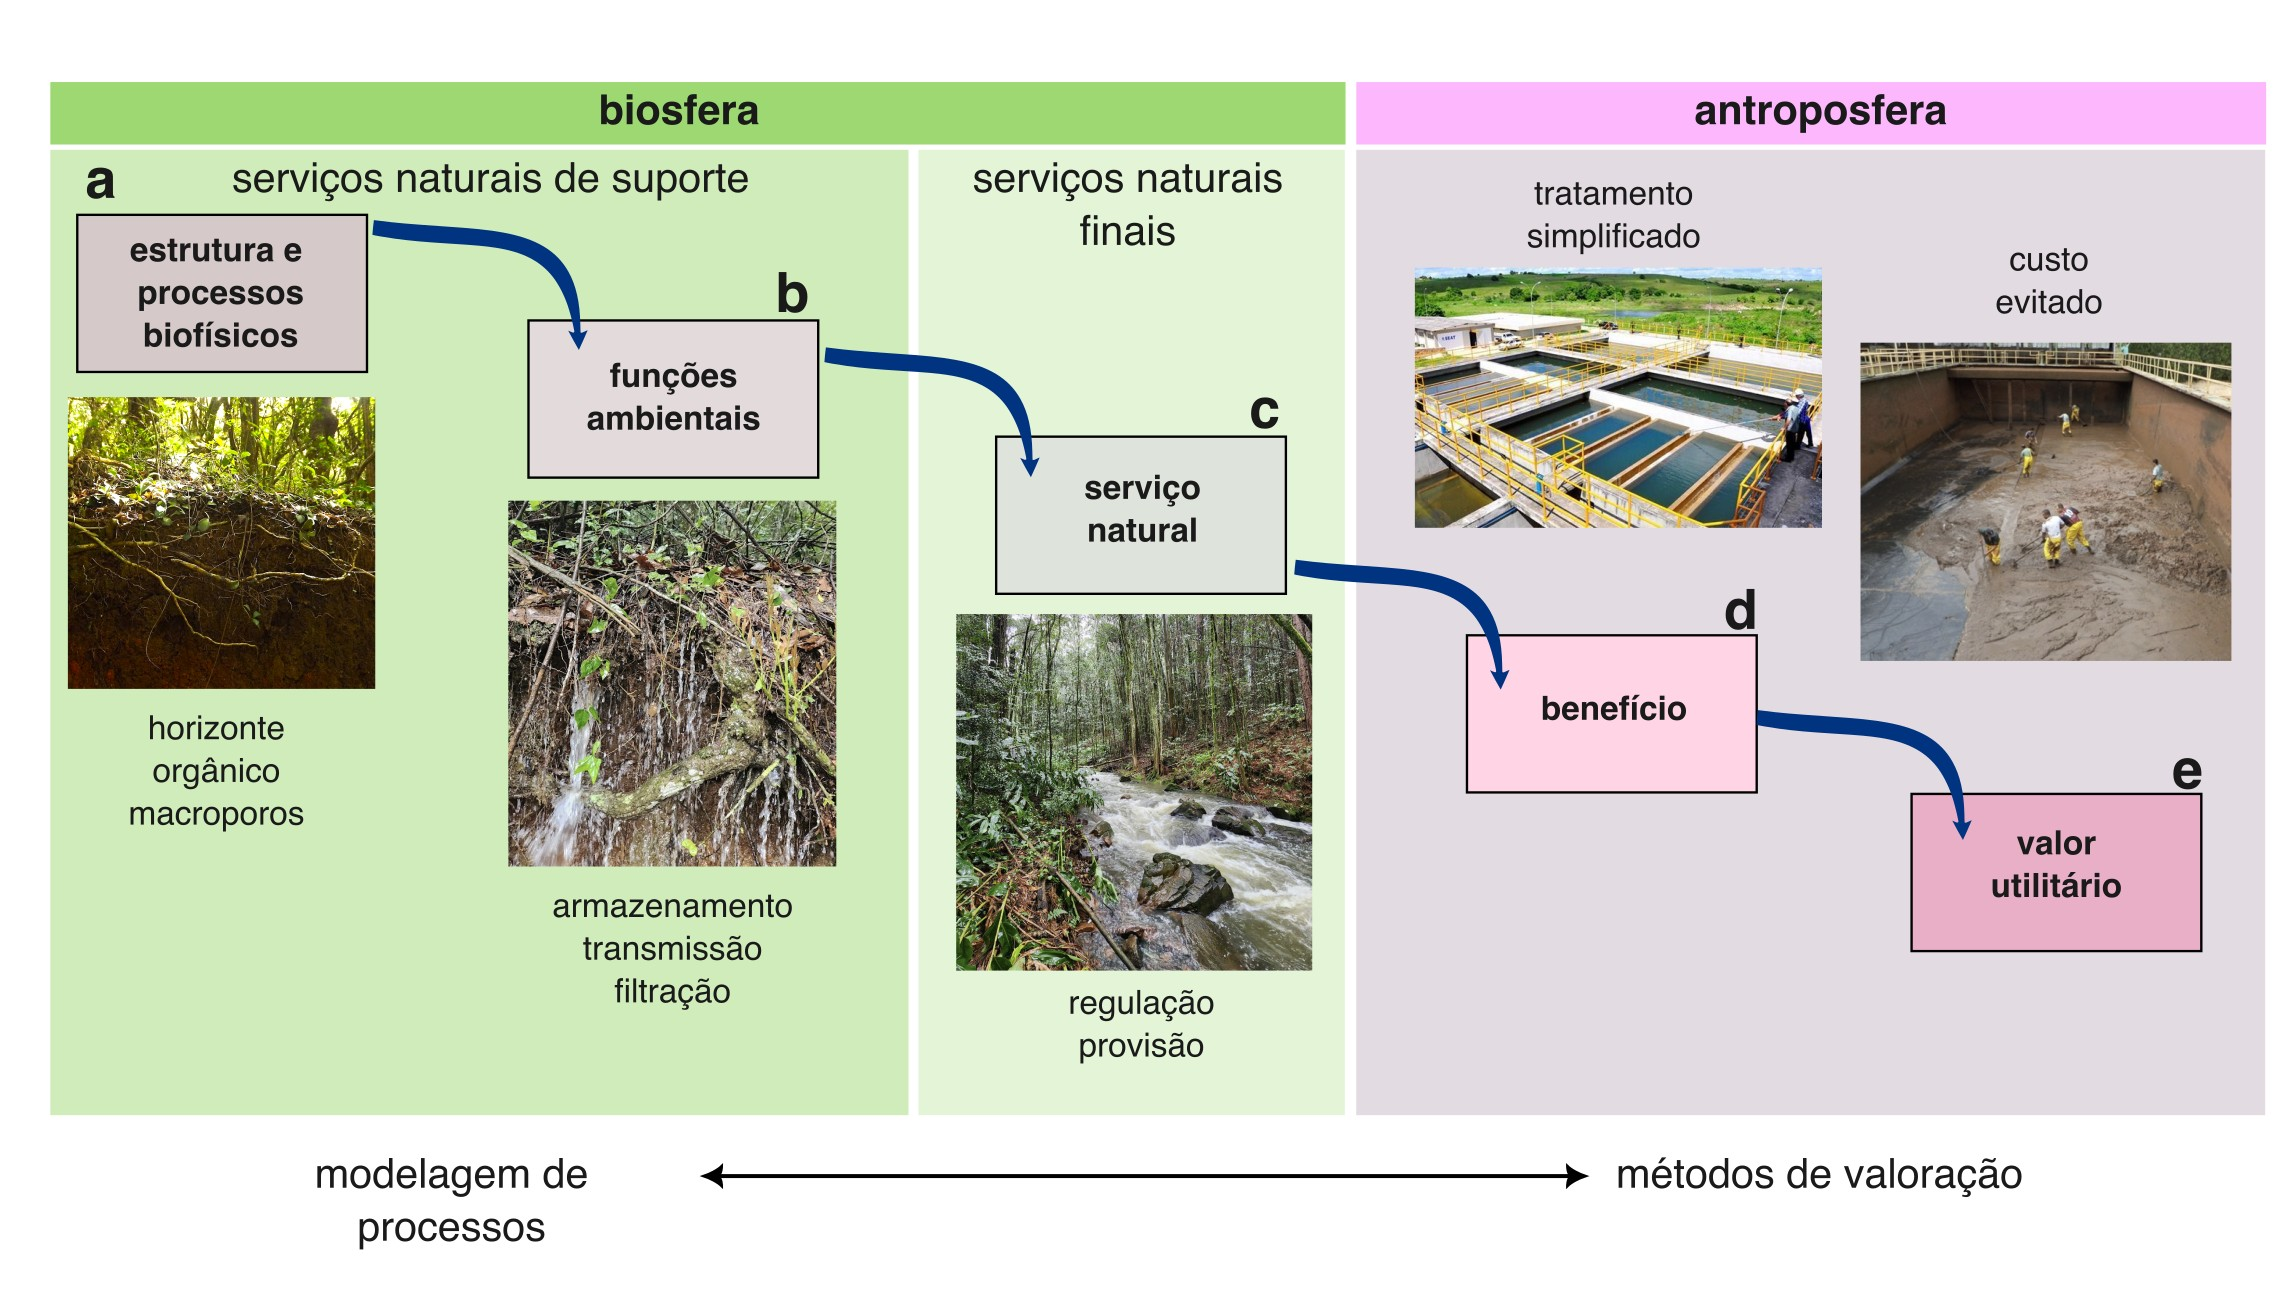
\includegraphics[width=0.98\linewidth]{figs/fig_cascade.jpg}		
\caption[O \gls{model} de cascata de serviços naturais]
{\textbf{---\;O \gls{casctmodel}.}
    O arcabouço conceitual mais moderno para entender os serviços ecossistêmicos é o modelo de cascata, proposto por Haines-Young \& Potschin (2010) \cite{haines-young2010}. Esse modelo descreve como os serviços naturais fluem até gerar benefícios para a sociedade em cinco etapas, com as primeiras três etapas na biosfera e as últimas duas etapas na antroposfera. Em cada extremo, é possível desenvolver estimativas quantitativas por modelos de processos e métodos de valoração.
    \;\textbf{a}\;---\;Base estrutural e processos biofísicos: representam os elementos fundamentais dos ecossistemas que sustentam suas funções, como características físicas e químicas. Por exemplo, isso inclui o horizonte orgânico do solo e a presença de macroporos.
    \;\textbf{b}\;---\;Funções ambientais: correspondem aos processos ecológicos que decorrem da dinâmica estrutural. No exemplo do solo, essas funções englobam o armazenamento, a transmissão e a filtração da água, processos fundamentais para a recarga dos aquíferos e a purificação natural da água.
    \;\textbf{c}\;---\;Serviços naturais finais: benefícios derivados diretamente das funções ambientais e que podem ser utilizados pela antroposfera, como a provisão de água limpa ou a perenidade dos cursos d'água para jusante.
    \;\textbf{d}\;---\;Benefício: refere-se ao valor utilitário decorrente dos serviços naturais, como a melhoria da saúde, segurança ambiental e suporte para atividades econômicas. No caso da água, por exemplo, um dos benefícios é o tratamento simplificado e menos custoso da água para abastecimento.
    \;\textbf{e}\;---\;Valor utilitário: representa a valoração econômica dos benefícios obtidos. Por exemplo, uma forma de valorar consiste em se estimar os custos evitados com a gestão de lodo e tratamento avançado de água, ou ainda a necessidade de se captar água de boa qualidade em um local mais distante.
}
\label{fig:eco:cascade} 		
\end{figure}

\par Os \gls{natserv} implicados pelo conceito de \gls{natcap} trouxeram desafios tanto nas frentes teóricas quanto na prática para o desenho de políticas de \gls{sustdev}. A ideia de serviço natural, sem definições claras, torna-se pouco palpável para influenciar decisões de alocação. Em contraste, o gerenciamento de recursos não-renováveis é muito mais evidente, pois o consumo desses recursos, com sua destruição ou transformação irreversível, os torna progressivamente escassos. Sabendo que uma jazida de carvão mineral inevitavelmente se esgotará, faz sentido elaborar estratégias de diversificação energética. Por outro lado, uma floresta tropical representa um \gls{natcap} que oferece uma vasta gama de serviços, muitos dos quais são difusos e beneficiam muito além dos seus habitantes ou visitantes, em diversas escalas. Os próprios \gls{recrenew} da floresta, como a madeira ou alimentos, resultam de \gls{natservprov}, que podem ser degradados por diversas razões, como colapsos ecológicos. Para desenhar instrumentos de gestão desses \gls{natserv}, como controle, incentivos e negociações, é necessário identificá-los, mensurá-los e atribuir-lhes \textbf{\gls{econval}}. Esse é um grande desafio do novo \gls{paradigma}, ainda que existam avanços recentes.

\par Um arcabouço conceitual mais moderno para se compreender os \gls{natserv} consiste no \textbf{\gls{casctmodel}}, proposto por Haines-Young \& Potschin (2010) \cite{haines-young2010, potschin2016}. Esse \gls{model} descreve como que os serviços ecossistêmicos fluem da natureza até gerar benefícios para a sociedade em cinco etapas principais: (1) estrutura e processo; (2) função; (3) serviço; (4) benefício; e (5) valor. As primeiras três etapas pertencem à \gls{biosf}, ressaltando a importância primordial da \textbf{\gls{biophysistrc}}, como florestas e zonas úmidas, que fornecem a base para o desenvolvimento de \textbf{\gls{ecoprocess}}, como a infiltração de água e a ciclagem de nutrientes. Esses processos, por sua vez, geram \textbf{\gls{envfunc}} que podem se tornar úteis para os seres humanos. Assim, o \gls{model} enfatiza que a função ambiental de um ecossistema, ou seja, sua \textit{capacidade} de realizar algo potencialmente útil para os seres humanos, não é automaticamente um serviço natural. Apenas quando essa função é considerada \textit{benéfica} para a sociedade é que ela se torna um serviço, como a \gls{gutility} da regulação de inundações em regiões densamente povoadas. A últimas duas etapas da cascata, por outro lado, pertencem à \gls{antroposf}. O \textbf{\gls{econbenefit}}, portanto, corresponde à manifestação concreta do \gls{welbeing} derivado desse serviço natural, como uma cidade menos vulnerável aos impactos de enchentes. Mas a percepção desse bem-estar depende do contexto e das necessidades humanas específicas, o que leva à variabilidade na avaliação do seu \textbf{valor econômico}. Por exemplo, o valor varia conforme as condições de oferta e demanda: diante da explosão populacional de roedores, o \gls{econval} do \gls{natservcontrol} é muito maior do que em períodos de normalidade. Além disso, nem todos os benefícios podem ser avaliados em termos se seu \gls{exchaval}, apresentando apenas \gls{useval}, como no caso dos \gls{natservcult}, que atuam diretamente sobre o bem-estar subjetivo, sem produtos materiais intermediários.

\subsection{Classificações de serviços naturais} \label{sec:natserv:sist}

\begin{figure}[t!] 
\centering				
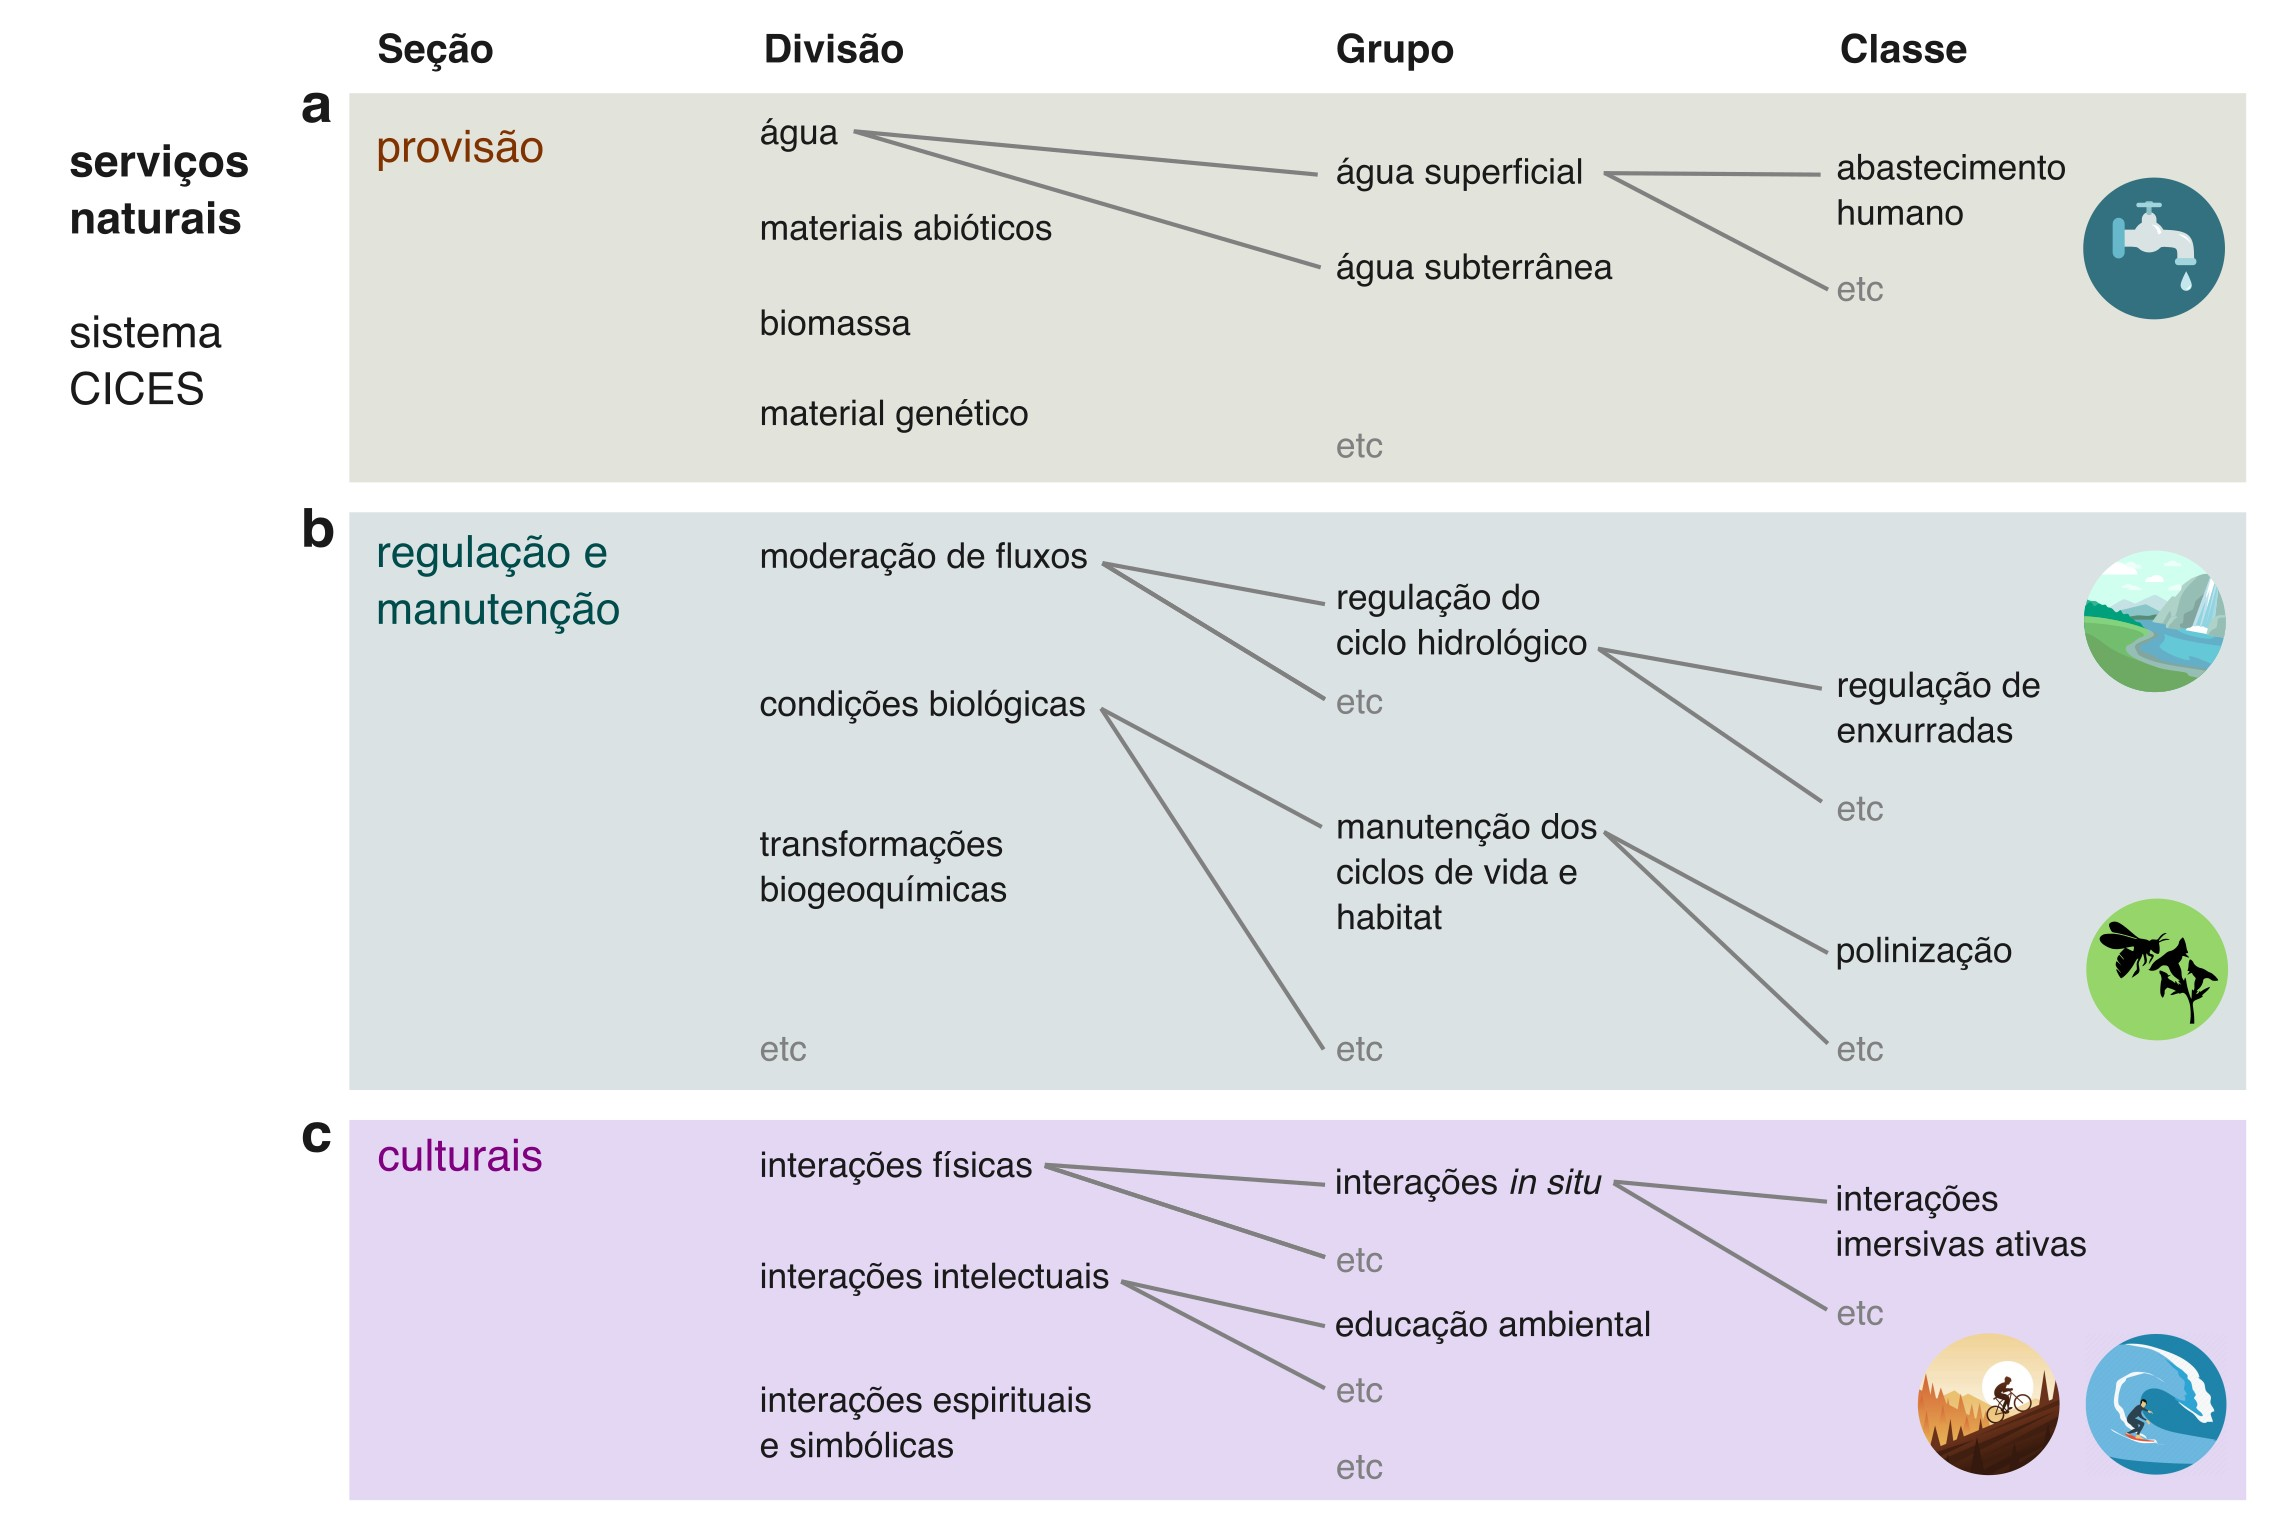
\includegraphics[width=0.98\linewidth]{figs/fig_cices.jpg}		
\caption[O sistema CICES de classificação de serviços naturais]
{\textbf{---\;O sistema CICES de classificação de serviços naturais}
    A Classificação Internacional Comum de Serviços Ecossistêmicos (CICES) oferece um sistema que categoriza os serviços ecossistêmicos em três seções principais: provisão, regulação e manutenção, e culturais. Cada seção é detalhada em divisões, grupos e classes.
    \;\textbf{a}\;---\;Os serviços naturais de provisão estão relacionados ao fornecimento direto de matérias primas (estoque-fluxos), como água e biomassa, essenciais para o abastecimento humano e outras atividades econômicas. Por exemplo, a água é classificada em subgrupos como água superficial e água subterrânea, que fornecem recursos fundamentais para o consumo humano, agricultura, etc.
    \;\textbf{b}\;---\;Os serviços naturais de regulação e manutenção incluem os fundos-serviços de processos e funções biogeoquímicas que garantem a qualidade ambiental e o funcionamento dos ciclos naturais. Esses serviços englobam a regulação do ciclo hidrológico, como a regulação de enxurradas, e a manutenção dos habitats para diversas espécies, como a polinização.
    \;\textbf{c}\;---\;Os serviços naturais culturais representam os serviços que proporcionam fundos-serviços imateriais, relacionados às interações físicas, intelectuais, espirituais e simbólicas entre seres humanos e a natureza. Entre esses serviços, estão atividades recreativas, como as interações no próprio ambiente natural, e as oportunidades de educação ambiental, que promovem o bem-estar e o enriquecimento cultural.
}
\label{fig:eco:natserv:cices} 		
\end{figure}

\par A largada da sistematização dos \gls{natserv} foi inciada por Daily \textit{et al.} (1997), especialmente no sentido de identificar e caracterizar os \gls{natserv}, mas também sobre os problemas de valoração \cite{daily1997}. Os autores definem esses serviços como \say{as condições e os processos pelos quais os ecossistemas naturais, e as espécies que os compõem, sustentam e promovem a vida humana.}. Eles trazem uma categorização pioneira, ainda que não tenham incluído detalhes sobre aspectos culturais, que separa os \textbf{\gls{natservgen}} dos \textbf{\gls{natservbiome}}. No caso dos serviços gerais, a lista inclui o \textbf{\gls{natservclim}} promovida pelos diversos ciclos biogeoquímicos (como do carbono, nitrogênio, fósforo e enxofre) e pelos ciclos da água dos sedimentos. Nessa lista, a biodiversidade é citada como um fator crítico para a estabilidade dos ecossistemas, garantindo maior resiliência a distúrbios. São mencionados também os \textbf{\gls{natservsoil}}, como a regulação do \gls{hydro_cicle}, suporte físico e fornecimento de nutrientes para plantas, além da decomposição de matéria orgânica, que recicla nutrientes e previne a proliferação de patógenos. Outros serviços gerais citados incluem o \textbf{\gls{natservpol}}, que sustenta a produção agrícola, e o \textbf{\gls{natservcontrol}}, promovido por predadores e parasitas que reduzem a necessidade de pesticidas, preservando a estabilidade da produção de alimentos. Os \gls{natserv} de biomas, por sua vez, realizam todos os serviços gerais mencionados, mas com as suas singularidades específicas em diferentes ecossistemas. Eles incluem os \gls{natserv} dos oceanos, os serviços das águas doces, os serviços das florestas e os serviços das pastagens naturais.

\par Outro marco histórico para a consolidação teórica e prática do conceito de \gls{natserv} foi o relatório \textit{Ecosystems and Human Well-being}, uma iniciativa das Nações Unidas concluída em 2005, também conhecido como o relatório da \acrfull{mea}\footnote{Avaliação Ecossistêmica do Milênio, em uma tradução livre do inglês.} \cite{MEA2005a}. Esse relatório avançou, em certa medida, o esforço de modelagem global dos \gls{natrec} divulgado em 1974 pelo Clube de Roma em \textit{Limites do crescimento} \cite{meadows1974}, trazendo dados mais detalhados sobre a distribuição e as mudanças dos ecossistemas. Na época, a avaliação destacou que aproximadamente 60\% dos \gls{natserv} estavam sendo degradados ou utilizados de forma insustentável, colocando em risco o bem-estar de populações em todo o planeta, especialmente as mais vulneráveis. Além de fornecer um dimensionamento extremamente relevante, o relatório \acrshort{mea} ajudou a consolidar a definição de \gls{natserv} como os \textit{benefícios diretos que as pessoas obtêm da natureza}. Vale destacar que o relatório \acrshort{mea} também consolidou o termo \textbf{\gls{ecoserv}}, que atualmente é o mais utilizado, embora existam variações como \textbf{\gls{envserv}}\footnote{Pessoalmente, eu prefiro a denominação \say{serviço natural}, não apenas por ser mais abrangente, mas por ser mais simples de ser compreendida pelo público leigo.}. Essa separação terminológica ainda não é totalmente clara na \gls{teoria}, mas há diferenças práticas e em marcos regulatórios. No Brasil, por exemplo, a Política Nacional de Pagamento por Serviços Ambientais faz a separação da seguinte maneira:

\begin{adjustwidth}{100pt}{0pt}
\medskip
\small 
(...)
Art. 2º Para os fins desta Lei, consideram-se:

I - ecossistema: complexo dinâmico de comunidades vegetais, animais e de microrganismos e o seu meio inorgânico que interagem como uma unidade funcional; 

II - serviços ecossistêmicos: benefícios relevantes para a sociedade gerados pelos ecossistemas, em termos de manutenção, recuperação ou melhoria das condições ambientais, (...)

III - \gls{envserv}: atividades individuais ou coletivas que favorecem a manutenção, a recuperação ou a melhoria dos serviços ecossistêmicos

-- Brasil (2021, p. 1) \cite{brasil2021}.
\medskip
\end{adjustwidth}
\noindent Apesar dessa definição oficial, o termo \say{serviço ambiental} também pode ser empregado para se referir aos benefícios obtidos de elementos naturais do ambiente construído, como em cidades. Nessa ótica, a arborização urbana, por exemplo, consistiria em uma forma de \textbf{\gls{greeninfra}} que oferece \gls{envserv}.

\par O relatório \acrshort{mea} preparou o caminho para a sistematização dos \gls{natserv} atualmente adotada pela \acrfull{cices}, ilustrada na Figura \ref{fig:eco:natserv:cices}, que foi mencionada na seção anterior: \gls{natservprov}, \gls{natservreg} e \gls{natservcult} \cite{Haines-young2018a}. Uma quarta categoria também foi articulada pelo \acrshort{mea}, que seriam os \textbf{\gls{natservsup}}, mas na \acrshort{cices} os serviços dessa classe foram desmembrados ou mantidos conceitualmente como processos precursores dos serviços em si. A sistematização proposta pelo \acrshort{mea} e pela \acrshort{cices} adota uma abordagem oposta à de Daily \textit{et al.} (1997), pois parte de uma perspectiva econômica e antropocêntrica, centrada na tipologia dos serviços, e não em sua origem na \gls{biosf}. Essa classificação orienta diretamente as decisões e avaliações relacionadas ao \gls{sustdev}, independentemente dos ecossistemas em questão. Nos serviços de provisão, a principal questão é se os materiais fornecidos pelo ecossistema estão sendo consumidos em uma taxa superior à sua capacidade de regeneração, como ocorre com a erosão dos solos agrícolas ou a pesca predatória. Nos serviços de regulação e manutenção, o foco é avaliar a capacidade do ecossistema de regular recursos, identificando até que ponto essa capacidade pode ser usada sem necessitar de medidas adicionais, como o armazenamento de água no solo para regular a disponibilidade hídrica ou a absorção de carbono pelos oceanos para mitigar o aquecimento global. Já nos serviços culturais, a questão central é identificar e valorar os benefícios imateriais que diferentes grupos obtêm do ecossistema, desde o lazer até o valor científico e educacional. Assim, essa sistematização enfatiza o aspecto econômico, facilitando a formulação de políticas para o \gls{sustdev}. Costanza (2008) sugere que isso é uma consequência inevitável da transição entre a \gls{biosf} e a \gls{antroposf}, sendo necessário se manter mais de um \gls{system} de classificação -- uns para mapear e identificar os serviços no lado da \gls{biosf} e outros para ajudar a tomada de decisão no lado da \gls{antroposf} \cite{costanza2008}.

\par A sistematização \acrshort{cices} apresenta uma estrutura hierárquica que organiza os \gls{natserv} em três níveis: as seções (nível mais alto), divisões (nível intermediário) e grupos (nível mais baixo), proporcionando uma padronização que facilita a contabilidade e o inventário ambiental. Sem um \gls{system} com esse detalhamento, seria praticamente inviável desenvolver políticas eficazes de gestão e valoração desses serviços. Com ele, projetos e ações podem ser explicitamente focadas em maximizar um ou mais \gls{natserv}. Pelo olhar hidrológico, por exemplo, a provisão de água é uma divisão dentro do serviço de provisão (código 4.2), que também abrange a provisão de biomassa e outros recursos abióticos. Essa divisão é subdividida em grupos, como a provisão de água superficial (código 4.2.1) e de água subterrânea (código 4.2.2). No caso da água superficial, as classes de serviços incluem a provisão de água potável (código 4.2.1.1), a provisão de água como insumo material (código 4.2.1.2) e a provisão de água para produção de energia (código 4.2.1.3). Esses serviços podem competir entre si, como ocorre em um reservatório que abastece uma usina hidrelétrica, onde o uso para geração de energia pode conflitar com a demanda por água potável ou industrial. No que se refere aos serviços de regulação e manutenção, a atenuação dos fluxos do \gls{hydro_cicle} na \acrshort{cices} resulta tanto de divisões bióticas (código 2.2.1.3) ou abióticas (código 5.2.1.2). A regulação biótica envolve os processos hidrológicos na escala das encostas, onde a fauna e flora influenciam a fragmentação superficial, favorecendo a infiltração. Já a regulação abiótica ocorre na escala de bacia hidrográfica, como nas planícies de inundação. Ambos os serviços demandam gestão, uma vez que podem ser prejudicados pela compactação do solo em encostas ou pela construção de diques nas planícies.

\subsection{Manifestações de valor utilitário} \label{sec:natserv:value}

\begin{figure}[t!] 
\centering				
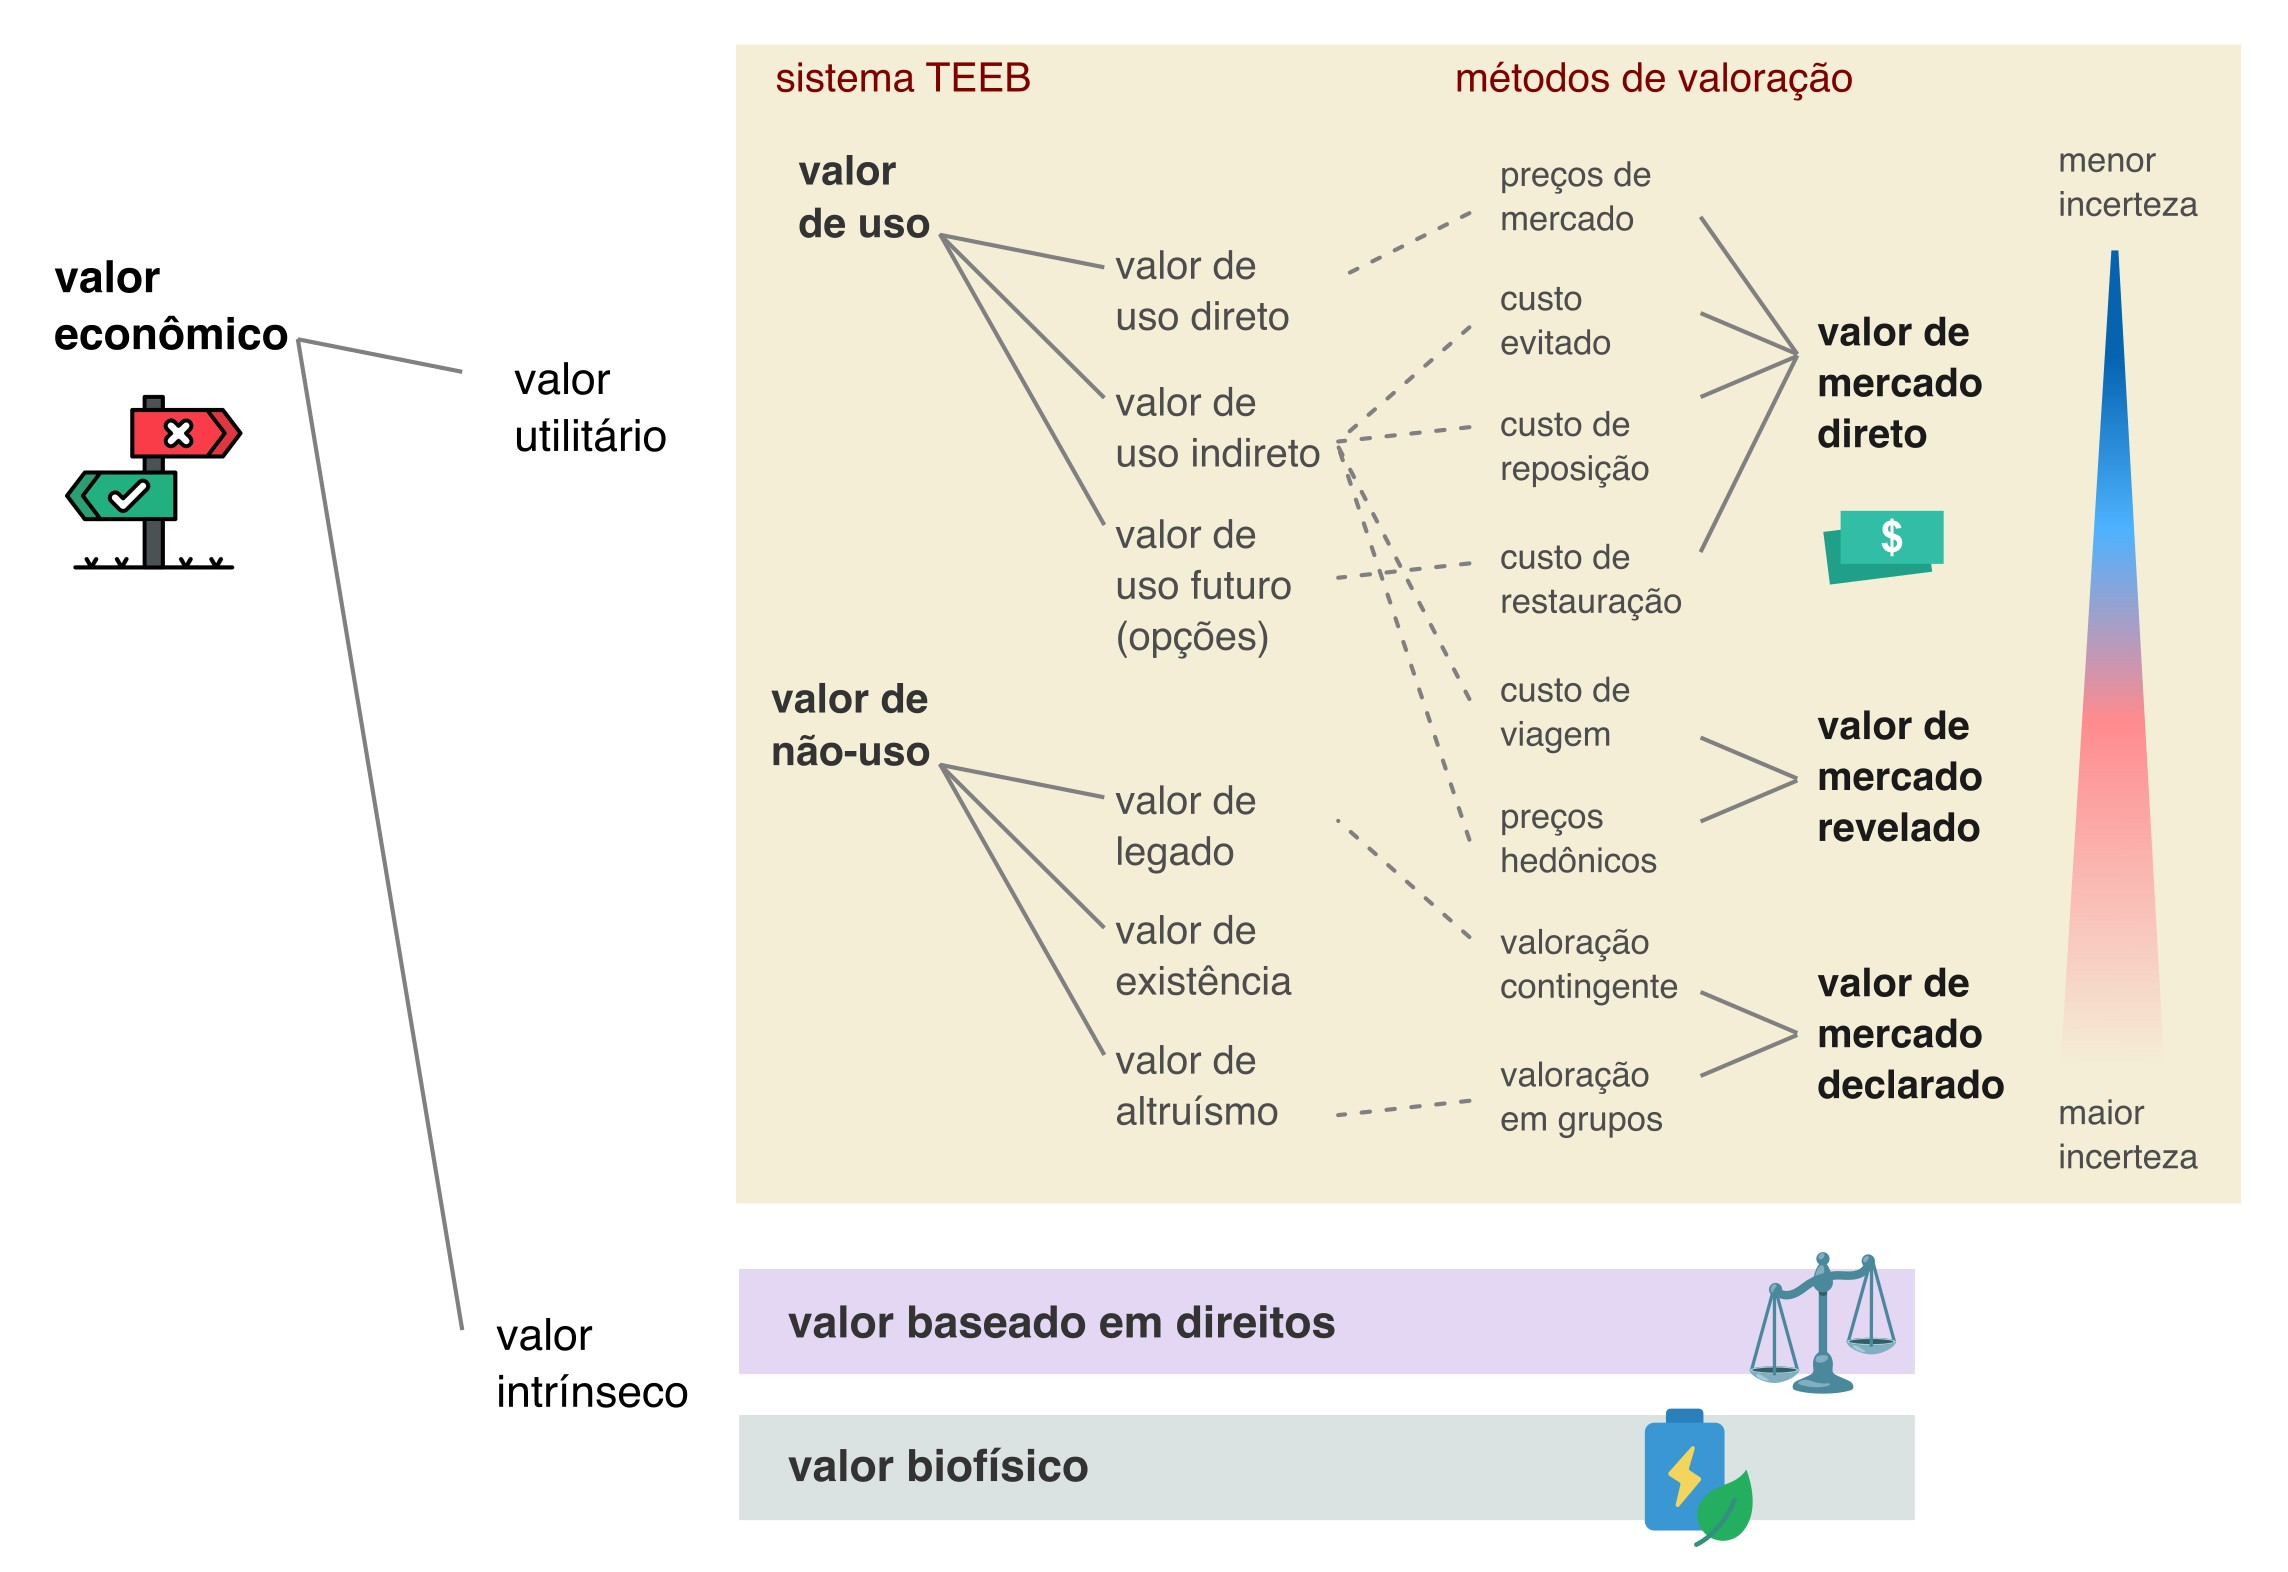
\includegraphics[width=0.98\linewidth]{figs/fig_teeb.jpg}		
\caption[As manifestações de valor utilitário]
{\textbf{---\;As manifestações de \gls{utilval}.}
    O valor utilitário consiste na métrica do paradigma ético utilitário, que elege a maximização da utilidade o seu objetivo supremo. No entanto outras formas de valor intrínseco são possíveis para orientar decisões econômicas, como o valor baseado em direitos (deontológico) e o valor biofísico, como a pegada de carbono, ou pegada hídrica.
    \;\textbf{a}\;---\;O valor utilitário, no sistema TEEB, envolve tanto o valor de uso e o valor de não-uso. O valor de uso inclui o uso direto (consuntivo e não-consuntivo); o valor de uso indireto (com intermediários), e; o valor de uso futuro, também chamado de valor das opções. O valor de não-uso consiste em valores utilitários que incluem o valor de legado; o valor de existência e o valor de altruísmo.
    \;\textbf{b}\;---\; Métodos de valoração incluem o valor de mercado direto, como preços e custos; valor de mercado indireto, como valor agregado da beleza cênica e custo de oportunidade do tempo de turistas, e; valor de mercado declarado, quando pesquisas são feitas para inferir o valor em mercados hipotéticos. Quanto mais direta for a valoração, menor é a incerteza associada ao método.
}
\label{fig:eco:natserv:value} 		
\end{figure}

\par A valoração de \gls{natserv} envolve as duas últimas etapas do \gls{model} de cascata: a avaliação do benefício e do \gls{econval}. Para entender esse processo com profundidade, é necessário se distanciar um pouco dos aspectos práticos e retornar para questões mais teóricas. Um \textit{valor} consiste em uma métrica empregada no processo de se fazer escolhas, que sempre são orientadas por um objetivo ético supremo. Por exemplo, se a honestidade é um valor importante para as relações humanas, então é \textit{melhor} se relacionar com pessoas íntegras do que com pessoas falsas (e sermos honestos, para não sermos \textit{desvalorizados} pelas outras pessoas). Valorar, portanto, consiste em calcular essa métrica com base nos fundamentos éticos pré-definidos. Nessa linha, o valor é tido como \textit{econômico} quando ele consiste na métrica para alocação de recursos escassos entre diferentes fins. Na \gls{ecoeco}, que se baseia no \gls{gutilitarism}, o \gls{econval} é um \textbf{\gls{utilval}} -- a \gls{gutility} ou sensação de \gls{welbeing}. Assim, apesar de todas as divergências que decorrem ao se adotar uma ontologia fisicalista, a \gls{ecoeco} se assemelha ao \gls{paradigma} econômico Neoclássico na sua dimensão ética. Ambas consideram a \gls{gutility} o \gls{ultimategoal}, ainda que a primeira reconhece o seu limite físico, e a segunda não.

\par O \gls{utilval}, contudo, não é a única forma possível de se avaliar escolhas em um contexto econômico, pois também existem formas de \textbf{\gls{intrisval}}, baseadas em direitos ou propriedades biofísicas \cite{kumar2012economics}. O \textbf{\gls{rightval}}\footnote{Também denominado na filosofia de valor deontológico, por não ser consequencialista, mas baseado em regrar definidas \textit{a priori}.} busca corrigir o \gls{antropoc} inerente ao \gls{gutilitarism}, que, por exemplo, não garante explicitamente que outras espécies não sejam extintas, desde que isso não prejudique a contabilidade final de \gls{welbeing}. Uma alternativa a esse enfoque é o \textbf{\gls{gbiocentrism}}, que, inspirado pela ética de Kant, defende que as outras espécies possuem o direito inalienável de existir. Nesse contexto, o \textbf{\gls{impercateg}} kantiano surge como um princípio moral que deve ser seguido, independentemente das consequências utilitárias. Esse princípio ético preconiza que decisões devem ser feitas \textit{como se} fossem derivadas de uma lei \textit{universalizável}. Assim, essa lógica pode ser aplicada para se estabelecer os direitos das outras espécies, pois se não gostamos da ideia de sermos usados ou exterminados por espécies mais avançadas tecnologicamente que nós, não deveríamos fazer isso com as espécies menos avançadas \cite{daily1997}. Já o \textbf{\gls{biophyval}} utiliza métricas físicas, como energia e materiais embutidos, para decidir sobre a alocação de recursos. Esse valor é uma versão ampliada do \textbf{valor de trabalho}, identificado na economia de Karl Marx. O conceito de \textbf{\gls{ecofootprint}}, por exemplo, atribui valor com base na carga material necessária para produzir um bem ou serviço, como as pegadas de carbono e hídrica. Essas valorações, embora filosoficamente distintas, não se excluem e podem se complementar em pelo emprego de \textbf{\gls{amcrit}} ou otimização multiobjetivo. Direitos biocêntricos, por exemplo, podem funcionar como restrições sobre a extensão do utilitarismo, enquanto a análise de ciclo de vida pode alterar a sensação de satisfação ou \gls{welbeing}. Após conhecer a enorme pegada de carbono de uma viagem de avião, talvez você se disponha a pagar por uma taxa extra para compensar as emissões.

\par As possíveis manifestações do \gls{utilval} dos \gls{natserv} são sistematicamente exploradas pela iniciativa \acrfull{teeb}, ilustrada na Figura \ref{sec:natserv:value}. Os autores dessa iniciativa definem o \textbf{\gls{tev}} como a soma de todas as formas de \gls{utilval}, organizadas em uma hierarquia de valores. Vale ressaltar que esse é um \gls{system} conceitual abrangente, aplicável tanto ao \gls{natcap} quanto ao antropogênico. Embora seja difícil e incerto obter o valor total de um dado recurso, isso geralmente não é necessário para orientar a tomada de decisão, pois os agentes econômicos costumam focar em alguns componentes específicos desse valor. Ao mesmo tempo, do ponto de vista da gestão do \gls{natcap}, o conceito de \gls{tev} é crucial para lembrar que as soluções de gestão devem considerar as perdas e ganhos entre os agentes que atuam em diferentes componentes.

\par O \gls{tev} se divide em \textbf{\gls{useval}} e \textbf{\gls{nonuseval}}. O \gls{useval}, como mencionado anteriormente, é um conceito relativamente intuitivo e bem estabelecido na \gls{gseconomics}. A \gls{marutilteo} sugere que o valor marginal de uso, ou seja, o benefício incremental obtido por unidade consumida, corresponde ao \textbf{valor de troca}, que varia conforme a oferta e demanda em mercados eficientes. Já o \gls{nonuseval} se refere à satisfação e ao bem-estar derivados de \textit{não} utilizar determinado bem ou serviço. Embora menos tangíveis, esses valores não podem ser ignorados, incluindo o \textbf{\gls{legval}}, que reflete a preocupação com a disponibilidade dos recursos para gerações futuras; o \textbf{\gls{altrval}}, que considera a equidade entre membros da geração atual; e o \textbf{\gls{existval}}, que diz respeito à satisfação obtida simplesmente pelo fato de saber que espécies e ecossistemas continuam a existir.

\par O \gls{useval} inclui tanto o \textbf{\gls{direcuseval}} quanto o \textbf{\gls{indirectuseval}}. O \gls{direcuseval} refere-se à interação explícita com o recurso, seja ele um serviço natural ou um bem de consumo convencional. Esse uso direto pode ser \textbf{\gls{useconsum}} ou \textbf{\gls{usenonconsun}}. O uso \gls{useconsum} envolve a transformação irreversível do recurso, que é o caso de todos os recursos do tipo estoque-fluxo. O uso \gls{usenonconsun}, por outro lado, relaciona-se mais com os recursos do tipo fundo-serviço, que não são transformados. Ao ir ao cinema, a pipoca tem um \gls{direcuseval} e \gls{useconsum}, mas o filme tem \gls{direcuseval} \gls{usenonconsun}. No contexto do \gls{natcap}, os \gls{natservprov} disponibilizam recursos com \gls{direcuseval} \gls{useconsum}, enquanto que os \gls{natservcult} exibem \gls{direcuseval} \gls{usenonconsun}. A água de um rio que abastece uma cidade, por exemplo, possui \gls{direcuseval} \gls{useconsum}, pois a água é transformada nesse processo. Mas as práticas de esportes náuticos nesse mesmo rio consiste apresenta \gls{direcuseval} \gls{usenonconsun}. O \gls{indirectuseval}, por outro lado, refere-se a interações menos explícitas com o recurso, onde o valor se manifesta por meio de processos intermediários que muitas vezes não são imediatamente visíveis. Usando o exemplo do cinema, dificilmente interagimos diretamente com a equipe de limpeza, mas a manutenção do ambiente limpo melhora nossa experiência. Nessa linha, no contexto do \gls{natcap}, o uso indireto está associado a \gls{natservreg}. A polinização realizada por insetos, por exemplo, é essencial para a agricultura, mas esse serviço não envolve uma interação direta entre o consumidor dos alimentos e os polinizadores. Da mesma forma, a infiltração de água nas encostas beneficia os usuários a jusante, que se beneficiam da disponibilidade de água limpa, mesmo sem interagir diretamente com o processo natural.

\par O \gls{direcuseval} e o \gls{indirectuseval} são ambos formas de \gls{useval} \textit{no presente}. No entanto, os autores da \acrshort{teeb} também destacam uma forma de \textbf{\gls{futuseval}}, conhecida como \textbf{\gls{optionval}}. Esse valor, no contexto do \gls{natcap}, está fortemente relacionado à capacidade dos ecossistemas de se manterem resilientes e se recuperarem de perturbações. Contudo, essa resiliência tem limites e pode ser comprometida quando o ecossistema é submetido a uma perturbação muito intensa, ultrapassando um \textbf{\gls{tippingpoint}}. A partir desse limiar crítico, o atrator do \gls{system} migra para uma nova região, que pode ser estável ou instável, resultando na perda ou degradação significativa dos \gls{natserv} previamente disponíveis. Um exemplo de mudança de regime estável-estável é a introdução de espécies invasoras, que alteram rapidamente o equilíbrio ecológico, reduzindo a biodiversidade. Nessa situação, a restauração do ecossistema original torna-se extremamente onerosa, pois o atrator do \gls{system} encontra-se em outro ponto ou região de estabilidade. Já uma mudança de regime estável-instável ocorre quando a erosão do solo progride de pequenos sulcos para grandes ravinas e voçorocas, com fortes retroações positivas que intensificam o processo de erosão cada vez mais. O \gls{optionval} reflete a \textbf{\gls{riskaversv}} de mudanças de regime no \gls{system}, que acarretariam custos exorbitantes. Nesse contexto, a \gls{uncert-episteme} — a falta de conhecimento sobre o \gls{system} — torna-se um fator crucial na avaliação desse valor, aumentando à medida que a ignorância sobre o comportamento do \gls{system} é reconhecida. O \gls{futuseval}, portanto, está diretamente ligado ao \textbf{\gls{precauprinci}}, que orienta que, em condições de alta incerteza sobre os pontos de não-retorno, as políticas devem ser guiadas por salvaguardas conservadoras.

\subsection{Métodos de valoração} \label{sec:natserv:valuemethos}

\par A determinação de cada componente do \gls{tev} envolve o uso de uma variedade de métodos, que avançam por estratégias incrementais, de acordo com as informações de \gls{useval} marginal (preços) disponíveis. É claro que limitações técnicas, metodológicas e de incerteza dos métodos de valoração aumentam conforme a escassez de informações disponíveis. Quando os \gls{natserv} estão fortemente vinculados a mercados reais, pode-se aplicar técnicas de \textbf{\gls{valuadm}}. Em situações em que os \gls{natserv} tem uma relação indireta com mercados reais, busca-se informações em mercados reais paralelos pela aplicação de técnicas de \textbf{\gls{valuarevpref}}. Por fim, diante da ausência completa de um mercado real ou paralelo, as alternativas de valoração lançam mão de técnicas de \textbf{\gls{valuastatpref}}, estimando o valor em mercados hipotéticos.

\par No caso mais básico, a \gls{valuadm} identifica as transações de mercado que estão vinculadas diretamente aos \gls{natserv}. Esse método se divide em três categorias principais: \textbf{\gls{valuaprice}}, \textbf{\gls{valuacost}} e \textbf{\gls{valuafuncprod}}. A \gls{valuaprice} de mercado relaciona-se com os \gls{natservprov} cujos produtos são negociados em mercados. A abordagem é a mais direta possível: o \gls{useval} marginal, direto e \gls{useconsum}, é o \gls{gprice} de mercado, que pode ser corrigido para se remover eventuais distorções. As abordagens baseadas em custos, mais associadas aos \gls{natservreg}, focam na estimativa dos gastos necessários para recriar os benefícios dos \gls{natserv} por meios artificiais. Entre essas técnicas estão o \textbf{\gls{valuaavoid}}, que considera os custos de produção que seriam incorridos na ausência dos \gls{natserv}; o \textbf{\gls{valuarepo}}, que estima o valor necessário para substituir o serviço em si por tecnologias artificiais; e \textbf{\gls{valuarest}}, que avalia os gastos para mitigar a perda dos \gls{natserv} ou restaurá-los. Por sua vez, as abordagens baseadas em funções de produção são as abordagens mais integradas possíveis dessa categoria, quando existe conhecimento suficiente pra fazer a conexão causal do desempenho dos \gls{natserv} sobre a produção de um bem ou serviço negociado em mercados. 

\par Na situação intermediária, as técnicas de preferência revelada baseiam-se na observação das escolhas individuais em mercados existentes que estão relacionados indiretamente ao serviço natural em questão. Ou seja, os agentes econômicos \textit{revelam} a \gls{gutility} do serviço por meio de suas escolhas. Os autores da \acrshort{teeb} ressaltam que as principais metodologias dentro desse escopo são o \textbf{\gls{valuatravcost}} e o \textbf{\gls{valuahedonpric}}, ambos fortemente relacionados com \gls{natservcult}, valores com uso direto e \gls{usenonconsun}. A estimativa de custos de viagem é essencial para valorar os serviços culturais relacionados com atividades turísticas e de lazer, que inclui despesas diretas e o \gls{opcost} do tempo. Assim, o valor de uma mudança na qualidade ou quantidade de um local recreativo pode ser inferido a partir da função de demanda estimada para as visitas. Por outro lado, a precificação hedônica utiliza informações sobre a demanda implícita por um atributo ambiental embutido em recursos que são negociados em mercados. Um exemplo típico desse \textit{valor agregado} é a beleza cênica altamente valorizada nos preços de imóveis com vistas para paisagens naturais. A instalação de turbinas eólicas e outros aspectos de poluição visual na paisagem podem causar a perda desse esse serviço natural cultural, fato que se manifesta pela desvalorização de imóveis, por exemplo.

\par Por fim, na ausência de informações disponíveis em mercados, as abordagens de preferência declarada simulam um mercado hipotético para os \gls{natserv} por meio de pesquisas que consideram mudanças na provisão desses serviços. Essas técnicas podem estimar tanto valores de uso quanto de não-uso, como o valor da existência ou \gls{legval}. Entre as técnicas disponíveis está o \textbf{\gls{valuacontg}}, que utiliza questionários para se inferir dos agentes econômicos a sua disposição a pagar por melhorias em um serviço natural ou a disposição a aceitar a degradação em um serviço natural, sendo duas faces da mesma moeda. Uma forma mais complexa consiste no método de \textbf{\gls{valuachoice}}, quando os respondentes dos questionários são submetidos a uma rede de escolhas possíveis, sinalizando melhor as relações declaradas de perdas e ganhos. Uma avaliação ainda mais robusta inclui a \textbf{\gls{valuagroups}}, quando diferentes grupos de agentes econômicos participam em um processo plural para deliberar o valor de um dado serviço ou recurso natural. Esse processo viabiliza, com abordagens multi-critério, a integração com outras métricas de valor e sistemas éticos mencionados acima.

\section{Serviços naturais hidrológicos} \label{chap:ecoeco:watersheds}

\begin{figure}[t!] 
\centering				
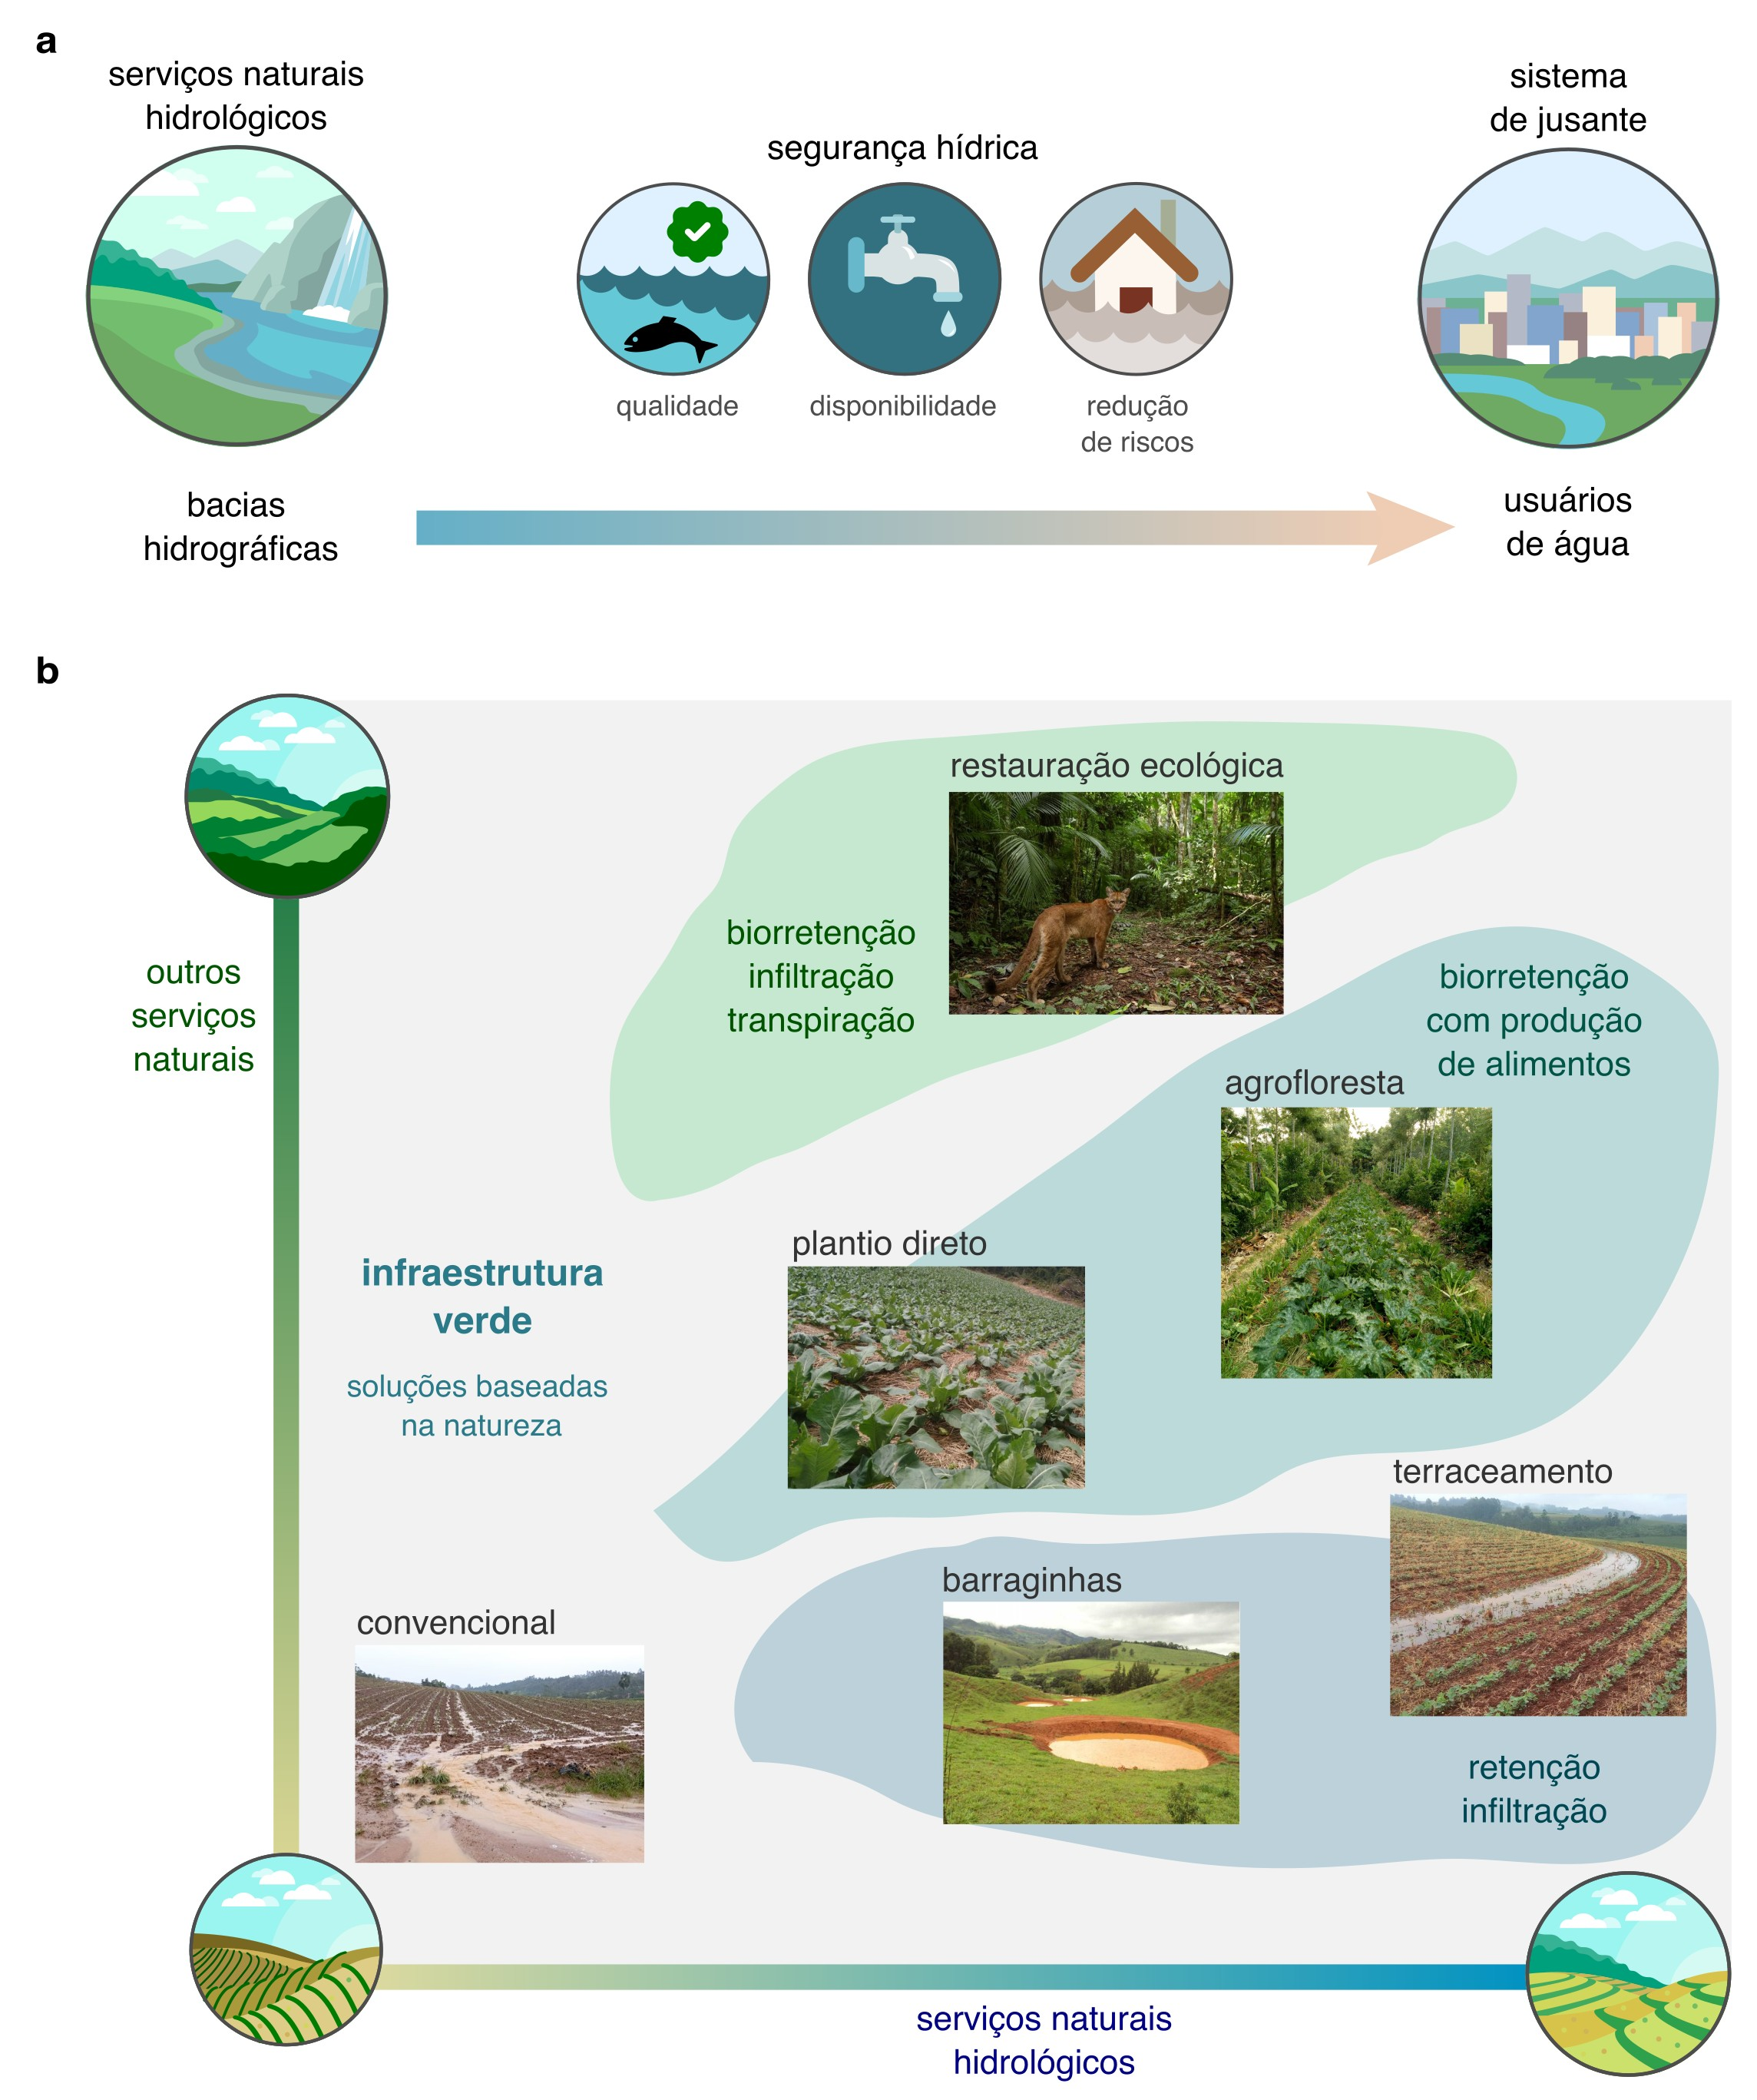
\includegraphics[width=0.98\linewidth]{figs/fig_sbn.jpg}		
\caption[Serviços naturais hidrológicos e a expansão de infraestrutura verde.]
{\textbf{---\;Serviços naturais hidrológicos e a expansão de infraestrutura verde.}
    O serviços naturais hidrológicos envolvem uma ampla gama de serviços naturais relacionados ao uso da terra tanto em bacias de ordem zero quanto em planícies de inundação.
    \;\textbf{a}\;---\;A principal característica dos serviços naturais hidrológicos é a sua escala de manifestação (a bacia hidrográfica) e a relação causal linear, beneficiando os usuários de água no sistema de jusante. Pelo enfoque o gerenciamento integrado de recursos hídricos, os serviços naturais hidrológicos contribuem para a segurança hídrica, melhorando a qualidade, aumentando a disponibilidade e reduzindo riscos associados aos processos hidrológicos.
    \;\textbf{b}\;---\;De forma complementar à infraestrutura cinza, a expansão de diversas formas de infraestrutura verde, que são soluções baseadas na natureza, pode ampliar a oferta dos serviços naturais hidrológicos. Em bacias de ordem zero, nas encostas, essas soluções incluem técnicas para aumentar a capacidade de retenção superficial e a capacidade de infiltração do solo. Aqui, surgem sinergias e trade-offs com outros serviços naturais. Por exemplo, a restauração ecológica implica em não produzir alimentos de forma convencional. Agroflorestas mediam tanto a produção de água com a produção de alimentos e ainda atendem em parte serviços naturais relacionados com a biodiversidade. 
}
\label{fig:eco:watersheds} 		
\end{figure}

\subsection{Segurança hídrica e infraestrutura verde} \label{sec:watersheds:watersecurity}

\par Com o advento da Economia Ecológica e seu conceito de capital natural, novas perspectivas surgiram para enquadrar o \textbf{gerenciamento integrado de recursos hídricos}, que, como paradigma de gestão e planejamento de bacias hidrográficas, visa garantir a \textbf{segurança hídrica}. As Nações Unidas definem segurança hídrica como a capacidade de uma população de: assegurar o acesso sustentável a quantidades adequadas de água de qualidade aceitável, necessárias para sustentar seu desenvolvimento socioeconômico; proteger contra poluição e desastres relacionados à água, e; preservar ecossistemas em um contexto de paz e estabilidade política \cite{cassin2021}. Na prática, garantir a segurança hídrica implica a necessidade de planejar e gerir programas, projetos e ações que, dentro dos contextos socioeconômicos e geopolíticos, garantam a disponibilidade, a qualidade e a regularidade da água em condições suficientes para atender demandas de múltiplos \textbf{usuários de água}, além de mitigar os riscos humanos associados a eventos extremos, como grandes enchentes e deslizamentos. Tais usuários em uma bacia hidrográfica representam diferentes agentes ou setores econômicos, que vão desde comunidades tradicionais, passando por companhias de abastecimento de água até setores econômicos como agricultura, indústria e produção de energia. Sob o paradigma ecológico-econômico, a água deixa de ser vista somente como um fator de produção para esses usuários e passa a ser reconhecida como um recurso comum fornecido pelo capital natural da bacia hidrográfica. Nessa ótica, torna-se claro que a alocação da água para os diferentes usos envolve, na verdade, o consumo de uma série de serviços naturais fornecidos pelos ecossistemas da bacia, denominados de \textbf{serviços naturais hidrológicos}. Smith \textit{et al.} (2006) \cite{Smith2006a} demonstram que esses serviços vão além da simples provisão de água, incluindo também a provisão de alimentos, a regulação dos fluxos de água e sedimentos, a qualidade da água, a mitigação de riscos hidrológicos e diversos serviços naturais culturais (Tabela \ref{tbl:waterserv}).

{\renewcommand{\arraystretch}{1.5}
\begin{table}[t!]
    \centering	
    \tiny
    \sffamily
    \rowcolors{2}{white}{rowgray}
    \begin{tabular}{ 
        >{\raggedright\arraybackslash}m{1.5cm} 
        >{\raggedright\arraybackslash}m{2.5cm}  
        >{\raggedright\arraybackslash}m{3.0cm}  
        >{\raggedright\arraybackslash}m{2.5cm}
        >{\raggedright\arraybackslash}m{2.5cm}
    }
    \toprule 
    \textbf{Seção} & \textbf{Serviços naturais hidrológicos} & \textbf{Atributos} & \textbf{Indicador de estado} & \textbf{Indicador de uso sustentável} \\ 
    \midrule 
    \textbf{Provisão} & Abastecimento de água & Precipitação, infiltração, armazenamento no solo, recarga, escoamento superficial, escoamento de base, aspectos bióticos e abióticos na qualidade da água & Capacidade de armazenamento de água (m³/m²), Concentrações de poluentes & Escoamento fluvial (m³/ano) \\ 
    
    \cline{2-5} 
     & Provisão de alimentos & Produção de cultivares, frutas, gado, plantas e animais comestíveis (ex: peixes, algas, invertebrados) & Uso de água agrícola (m³/ha), Estoque de peixes (kg/m³) & Uso máximo sustentável de água para irrigação (m³/ano), Produtividade líquida (kg/ha/ano) \\ 
    
    \cline{2-5}
     & Bens não alimentares & Produção de matérias-primas (ex: madeira, junco), produção de medicamentos & Quantidades disponíveis (kg/ha/ano) & Colheita máxima sustentável (kg/ha/ano) \\ 
    
    \cline{2-5} & Energia hidrelétrica & Vazão para geração de energia & Capacidade de armazenamento de leitos de rios e lagos (m³/m²), Declividade (grau), Elevação (m) & Produção máxima sustentável de energia (kWh/ano) \\ 
    
    \textbf{Regulação} & Regulação dos fluxos de água & Armazenamento e liberação (especialmente por florestas e áreas úmidas), Armazenamento de água por rios, lagos e áreas úmidas, Recarga e descarga de água subterrânea & Capacidade de infiltração (mm/h), Capacidade de armazenamento da zona vadosa (m³/m²) & Volume do escoamento de base (m³/ano) \\ 
    
    \cline{2-5}
    & Mitigação de riscos & Redução de picos de enchentes e danos por tempestades, Proteção costeira, Estabilidade de encostas & Capacidade máxima natural de armazenamento de água (m³/m²) & Extensão (km²) e valor econômico (\$/km²/ano) protegido de inundações \\ 
    
    \cline{2-5}
    & Controle da erosão e sedimentação & Proteção do solo pela vegetação e biota do solo & Capacidade de infiltração (mm/h), Comprimento da encosta (m), Terras áridas (\%) & Perda de solo anual (kg/ha/ano), Armazenamento de sedimentos (kg/m²/ano) \\ 
    
    \cline{2-5}
    & Purificação da água & Redução do assoreamento de rios e lagos, Absorção e liberação de nutrientes pelos ecossistemas, Remoção de matéria orgânica, sais, poluentes & Carga de nitrogênio (kg/ha), Carga de sólidos dissolvidos totais (kg/m²), Condutividade elétrica (\(\mu\)S/cm) & Taxa de Desnitrificação (kg/ha/ano) \\ 
    
    \cline{2-5}
    & Habitat para a vida selvagem & Habitats de vida selvagem e de reprodução & Espécies residentes e endêmicas (unidades), Área superficial por tipo de ecossistema (ha), Índice de qualidade de habitat (-) & Aumento ou declínio no tamanho da população de espécies (unidades) \\ 
    
    \cline{2-5} 
    & Fluxos ecológicos & Manutenção do regime de fluxos do rio & Área de habitats críticos (ha), Descarga por estação (m³/dia) & Espécies e população de peixes, Captura total de peixes (t/ano) \\ 
    
    \textbf{Cultural} & Beleza cênica e atividades recreativas & Qualidade e características da paisagem, Valor recreativo & Apreciação declarada, Valor recreativo (ex: taxas de entrada, \$/visita) & Casas em orlas (unidades/km), Visitantes (unidades/ano) \\ 
    
    \cline{2-5} 
    & Patrimônio e identidade & Características da paisagem ou espécies & Significado cultural e senso de pertencimento & Visitantes (unidades/ano) \\ 
    
    \cline{2-5} 
    & Inspiração espiritual e artística & Valor inspirador de características da paisagem e espécies & Livros e pinturas usando o rio ou a região como inspiração & Peregrinos (unidades/ano) \\ 
    
    \bottomrule
    \end{tabular}
    \caption[Os serviços naturais hidrológicos]{
        \textbf{Serviços naturais hidrológicos}\; --- \;Relação dos serviços naturais hidrológicos, principais atributos, indicadores de estado e indicadores de uso sustentável. Adaptado de Smith \textit{et al.} (2006) \cite{Smith2006a}.}
    \label{tbl:waterserv}
\end{table}
}

\par Evidentemente, a extensão espacial dos serviços naturais hidrológicos está diretamente vinculada à bacia hidrográfica, o que os diferencia de outros serviços ecossistêmicos, como a regulação climática (que ocorre em escala global). A dinâmica de montante para jusante nas bacias hidrográficas gera uma cadeia causal de respostas hidrológicas, que se traduz economicamente em externalidades, tanto positivas quanto negativas. Esses efeitos variam conforme o estado de conservação dos serviços naturais nas áreas de montante e o uso desses serviços nas regiões de jusante. Seguindo o modelo de cascata (Figura \ref{fig:eco:cascade}), fica claro que os serviços hidrológicos são frutos da interação entre a vegetação, o solo, a geologia e a topografia, as estruturas biofísicas e os processos que geram as funções ambientais. Como discutido no Capítulo \ref{chap:hydrology}, os processos hidrológicos que ocorrem nas encostas e nas bacias de ordem zero são a fonte original de grande parte dos serviços naturais hidrológicos. Em bacias de grandes rios, porém, esses serviços naturais também se manifestam a partir de processos como a inundação de planícies e o funcionamento ecológico das áreas úmidas, que também contribuem na regulação do ciclo hidrológico. Reconhecer esse fluxo de externalidades cria a oportunidade de gerenciar esse capital natural de forma a solucionar o problema do livre acesso e evitar a tragédia dos comuns. As políticas de gestão, nesse sentido, devem desenhar e reforçar conexões estratégicas entre os usuários da água nas áreas de jusante e os agentes econômicos responsáveis pela conservação e manejo nas encostas, localizado na região de montante. O objetivo supremo, por consequência, é maximizar o bem-estar humano, otimizando as ações antrópicas na bacia hidrográfica dentro do limite econômico.

\par Em um mundo de urbanização acelerada, a segurança hídrica depende principalmente da gestão dos mananciais que abastecem as cidades \cite{Liu2024}. Nessa linha, o relatório do Banco Mundial de Dudley \textit{et al.} (2003) \cite{Dudley2003a} consolidou a importância da gestão dos serviços naturais hidrológicos em áreas de mananciais, destacando que áreas protegidas com florestas bem manejadas em geral melhoram tanto a qualidade quanto a quantidade de água fornecida. O estudo mostrou que florestas naturais, especialmente as bem conservadas, oferecem água de maior qualidade, com menos sedimentos e poluentes, em comparação a outras áreas de captação. Além disso, florestas tropicais nativas e maduras podem aumentar a vazão de água, embora florestas jovens e plantações exóticas possam reduzir esse fluxo. O relatório também revelou que cerca de um terço (33 de 105) das maiores cidades do mundo captavam água diretamente de áreas protegidas, enquanto outras cinco dependiam de bacias hidrográficas distantes que incluem áreas protegidas, e pelo menos oito cidades captavam água de florestas manejadas com foco no abastecimento hídrico. Os autores sugeriram que, apesar dos benefícios dessas áreas para o abastecimento urbano e a biodiversidade, o valor econômico dos serviços hidrológicos ainda era subestimado. O relatório propôs a criação de mecanismos financeiros, como a cobrança de taxas de usuários, para ajudar a custear a proteção e manejo dessas áreas, o que hoje se enquadra nos incentivos por Pagamento por Serviços Ambientais (mais detalhes adiante). 

\par Com o papel dos serviços naturais hidrológicos bem estabelecido, a maximização da segurança hídrica passou a ser cada vez mais concebida no gerenciamento integrado de recursos hídricos através da complementação entre o capital antropogênico e o capital natural \cite{un2018}. As cidades, por exemplo, dependem da \textbf{infraestrutura cinza} para obter água potável, como barragens de armazenamento, estações de bombeamento e tratamento, entre outros. No entanto, a vegetação e o solo presentes na bacia hidrográfica, acima do ponto de captação, funcionam como uma \textbf{infraestrutura verde}, que reduz a intensidade de enxurradas nas encostas, um processo de resposta rápida com alto potencial erosivo. Em termos hidrológicos, isso ocorre principalmente devido à alta capacidade de infiltração do solo das florestas, como visto no Capítulo \ref{chap:hydrology}. O alto grau de fragmentação da superfície nas florestas também revela uma relativamente maior capacidade de retenção superficial efetiva, contribuindo para controlar as enxurradas de chuvas que excedem a capacidade de infiltração do solo. A Tabela \ref{tbl:nbs} resume as possibilidades de ações que as infraestruturas verdes oferecem sob o contexto de diferentes serviços naturais, em diferentes escalas de ação, comparando com seus correspondentes complementares da infraestrutura cinza.

\par O arranjo que alia infraestruturas verdes e cinzas, vem sendo cada vez mais enquadrado pelo conceito de \acrfull{nbs}, práticas que se inspiram ou fazem uso direto de processos naturais para melhorar a gestão da água, a produção de alimentos e a conservação da biodiversidade \cite{un2018, fao2019}. A ideia subjacente às \acrshort{nbs} integra conceitos já estabelecidos, como a engenharia ecológica, manejo conservacionista do solo e abordagens de gestão ambiental. Além disso, está alinhada aos princípios da Economia Ecológica, que reconhece a importância central do capital natural para o desenvolvimento sustentável \cite{nesshover2017}. Mas o diferencial do conceito das \acrshort{nbs} está no fato de que ele não necessariamente requer a preservação de um capital natural prístino e intocável, como florestas nativas, mas que expande o raio de ações ao se \textit{inspirar} em processos naturais, permitindo se projetar uma \textit{transição} ecológica que favoreça a \textit{reprodução} desses processos, mesmo em paisagens antropizadas. Por exemplo, uma lavoura que adota técnicas de plantio direto com terraços e cordões de biorretenção e infiltração reproduz uma estrutura biofísica análoga aos processos de infiltração observados em áreas de floresta nativa. Assim, as \acrshort{nbs} facilitam a restauração de ecossistemas e a recuperação de serviços ambientais ao integrar práticas que imitam funções ecológicas essenciais em ambientes manejados. A silvicultura ou a agrofloresta, com o plantio de árvores exóticas não invasoras, também pode contribuir para a recuperação de solos degradados, regenerando o horizonte orgânico e preparando o solo para a regeneração da mata nativa em etapas subsequentes. Dessa forma, as \acrshort{nbs} promovem uma transição gradual rumo ao limite econômico, sem depender exclusivamente de ecossistemas naturais intactos.

{\renewcommand{\arraystretch}{1.5}
\begin{table}[t!]
    \centering	
    \tiny
    \sffamily
    \rowcolors{2}{white}{rowgray}
    \begin{tabular}{ 
         >{\raggedright\arraybackslash}m{2.5cm}  
         >{\raggedright\arraybackslash}m{3.5cm}  
         >{\raggedright\arraybackslash}m{1.0cm}
         >{\raggedright\arraybackslash}m{1.0cm}
         >{\raggedright\arraybackslash}m{1.0cm}
         >{\raggedright\arraybackslash}m{2.5cm}
    }
    \toprule 
    \textbf{Problema de gestão/serviço natural} & \textbf{Solução de infraestrutura verde} & \textbf{Encostas} & \textbf{Planície} & \textbf{Cidades} & \textbf{Solução de infraestrutura cinza correspondente}\\ 
    \midrule
    \textbf{Abastecimento de água (regulação de fluxo)} & Reflorestamento e conservação florestal & x &  &  & Barragens e bombeamento de água subterrânea \\
    \cline{2-5}
    & Reconectar rios com planícies de inundação & x & x &  & Sistemas de distribuição de água \\
    \cline{2-5}
    & Restauração/conservação de áreas úmidas & x & x & x &  \\
    \cline{2-5}
    & Construção de áreas úmidas &  & x & x &  \\
    \cline{2-5}
    & Captação da água da chuva &  &  & x &  \\
    \cline{2-5}
    & Biorretenção e infiltração & x &  & x &  \\
    \cline{2-5}
    & Pavimentos permeáveis &  &  & x &  \\
    
    \textbf{Purificação de água (regulação da qualidade)}& Reflorestamento e conservação florestal & x &  &  & Estação de tratamento de água \\
    \cline{2-5}
    & Reconectar rios a planícies de inundação & x & x &  &  \\
    \cline{2-5}
    & Zona ripária & x &  &  &  \\
    \cline{2-5}
    & Restauração/conservação de áreas úmidas & x & x & x &  \\
    \cline{2-5}
    & Construção de áreas úmidas &  & x & x &  \\
    \cline{2-5}
    & Biorretenção e infiltração & x &  & x &  \\
    \cline{2-5}
    & Pavimentos permeáveis &  &  & x &  \\
    
    \textbf{Controle de erosão (regulação da qualidade)}& Reflorestamento e conservação florestal & x &  &  & Reforço de encostas \\
    \cline{2-5}
    & Zona ripária & x &  &  &  \\
    \cline{2-5}
    & Reconectar rios a planícies de inundação & x & x &  &  \\
    \cline{2-5}
    & Restauração/conservação de áreas úmidas & x & x & x &  \\
    \cline{2-5}
    & Construção de áreas úmidas &  & x & x &  \\
    
    \textbf{Controle de temperatura da água (regulação da qualidade)}& Reflorestamento e conservação florestal & x &  &  & Barragens \\
    \cline{2-5}
    & Zona ripária & x &  &  &  \\
    \cline{2-5}
    & Reconectar rios a planícies de inundação & x & x &  &  \\
    \cline{2-5}
    & Restauração/conservação de áreas úmidas & x & x & x &  \\
    \cline{2-5}
    & Construção de áreas úmidas &  & x & x &  \\
    \cline{2-5}
    & Sombreamento de cursos d'água &  &  & x &  \\
    
    \textbf{Controle biológico (regulação da qualidade)}& Reflorestamento e conservação florestal & x &  &  & Estação de tratamento de água \\
    \cline{2-5}
    & Zona ripária & x &  &  &  \\
    \cline{2-5}
    & Reconectar rios a planícies de inundação & x & x &  &  \\
    \cline{2-5}
    & Restauração/conservação de áreas úmidas & x & x & x &  \\
    \cline{2-5}
    & Construção de áreas úmidas &  & x & x &  \\
    
    \textbf{Controle de inundações fluviais (regulação de distúrbios)}& Reflorestamento e conservação florestal & x &  &  & Barragens e diques \\
    \cline{2-5}
    & Zona ripária & x &  &  &  \\
    \cline{2-5}
    & Reconectar rios a planícies de inundação & x & x &  &  \\
    \cline{2-5}
    & Restauração/conservação de áreas úmidas & x & x & x &  \\
    \cline{2-5}
    & Construção de áreas úmidas &  & x & x &  \\
    \cline{2-5}
    & Canais de extravasamento &  & x &  &  \\
    
    \textbf{Manejo de águas pluviais (regulação de distúrbios)}& Telhados verdes &  &  & x & Tubulações de micro e macrodrenagem  \\
    \cline{2-5}
    & Biorretenção e infiltração &  &  & x & \\
    \cline{2-5}
    & Captação da água da chuva &  &  & x &  \\
    \cline{2-5}
    & Pavimentos permeáveis &  &  & x &  \\
    
    \bottomrule
    \end{tabular}
    \caption[Infraestrutura verde para serviços naturais hidrológicos]{
    \textbf{Solução de infraestrutura verde para melhorar os serviços naturais hidrológicos}\; --- \;Relação sistematizada entre serviços hidrológicos naturais, infraestrutura verde, escalas de aplicação (bacia, planície de inundação ou cidades), e a solução de infraestrutura cinza correspondente. Adaptado de Cassin \textit{et al.} (2021) \cite{cassin2021}.
    }
    \label{tbl:nbs}
\end{table}
}

\subsection{Esquemas de pagamentos} \label{sec:watersheds:pes}

\begin{figure}[t!] 
\centering				
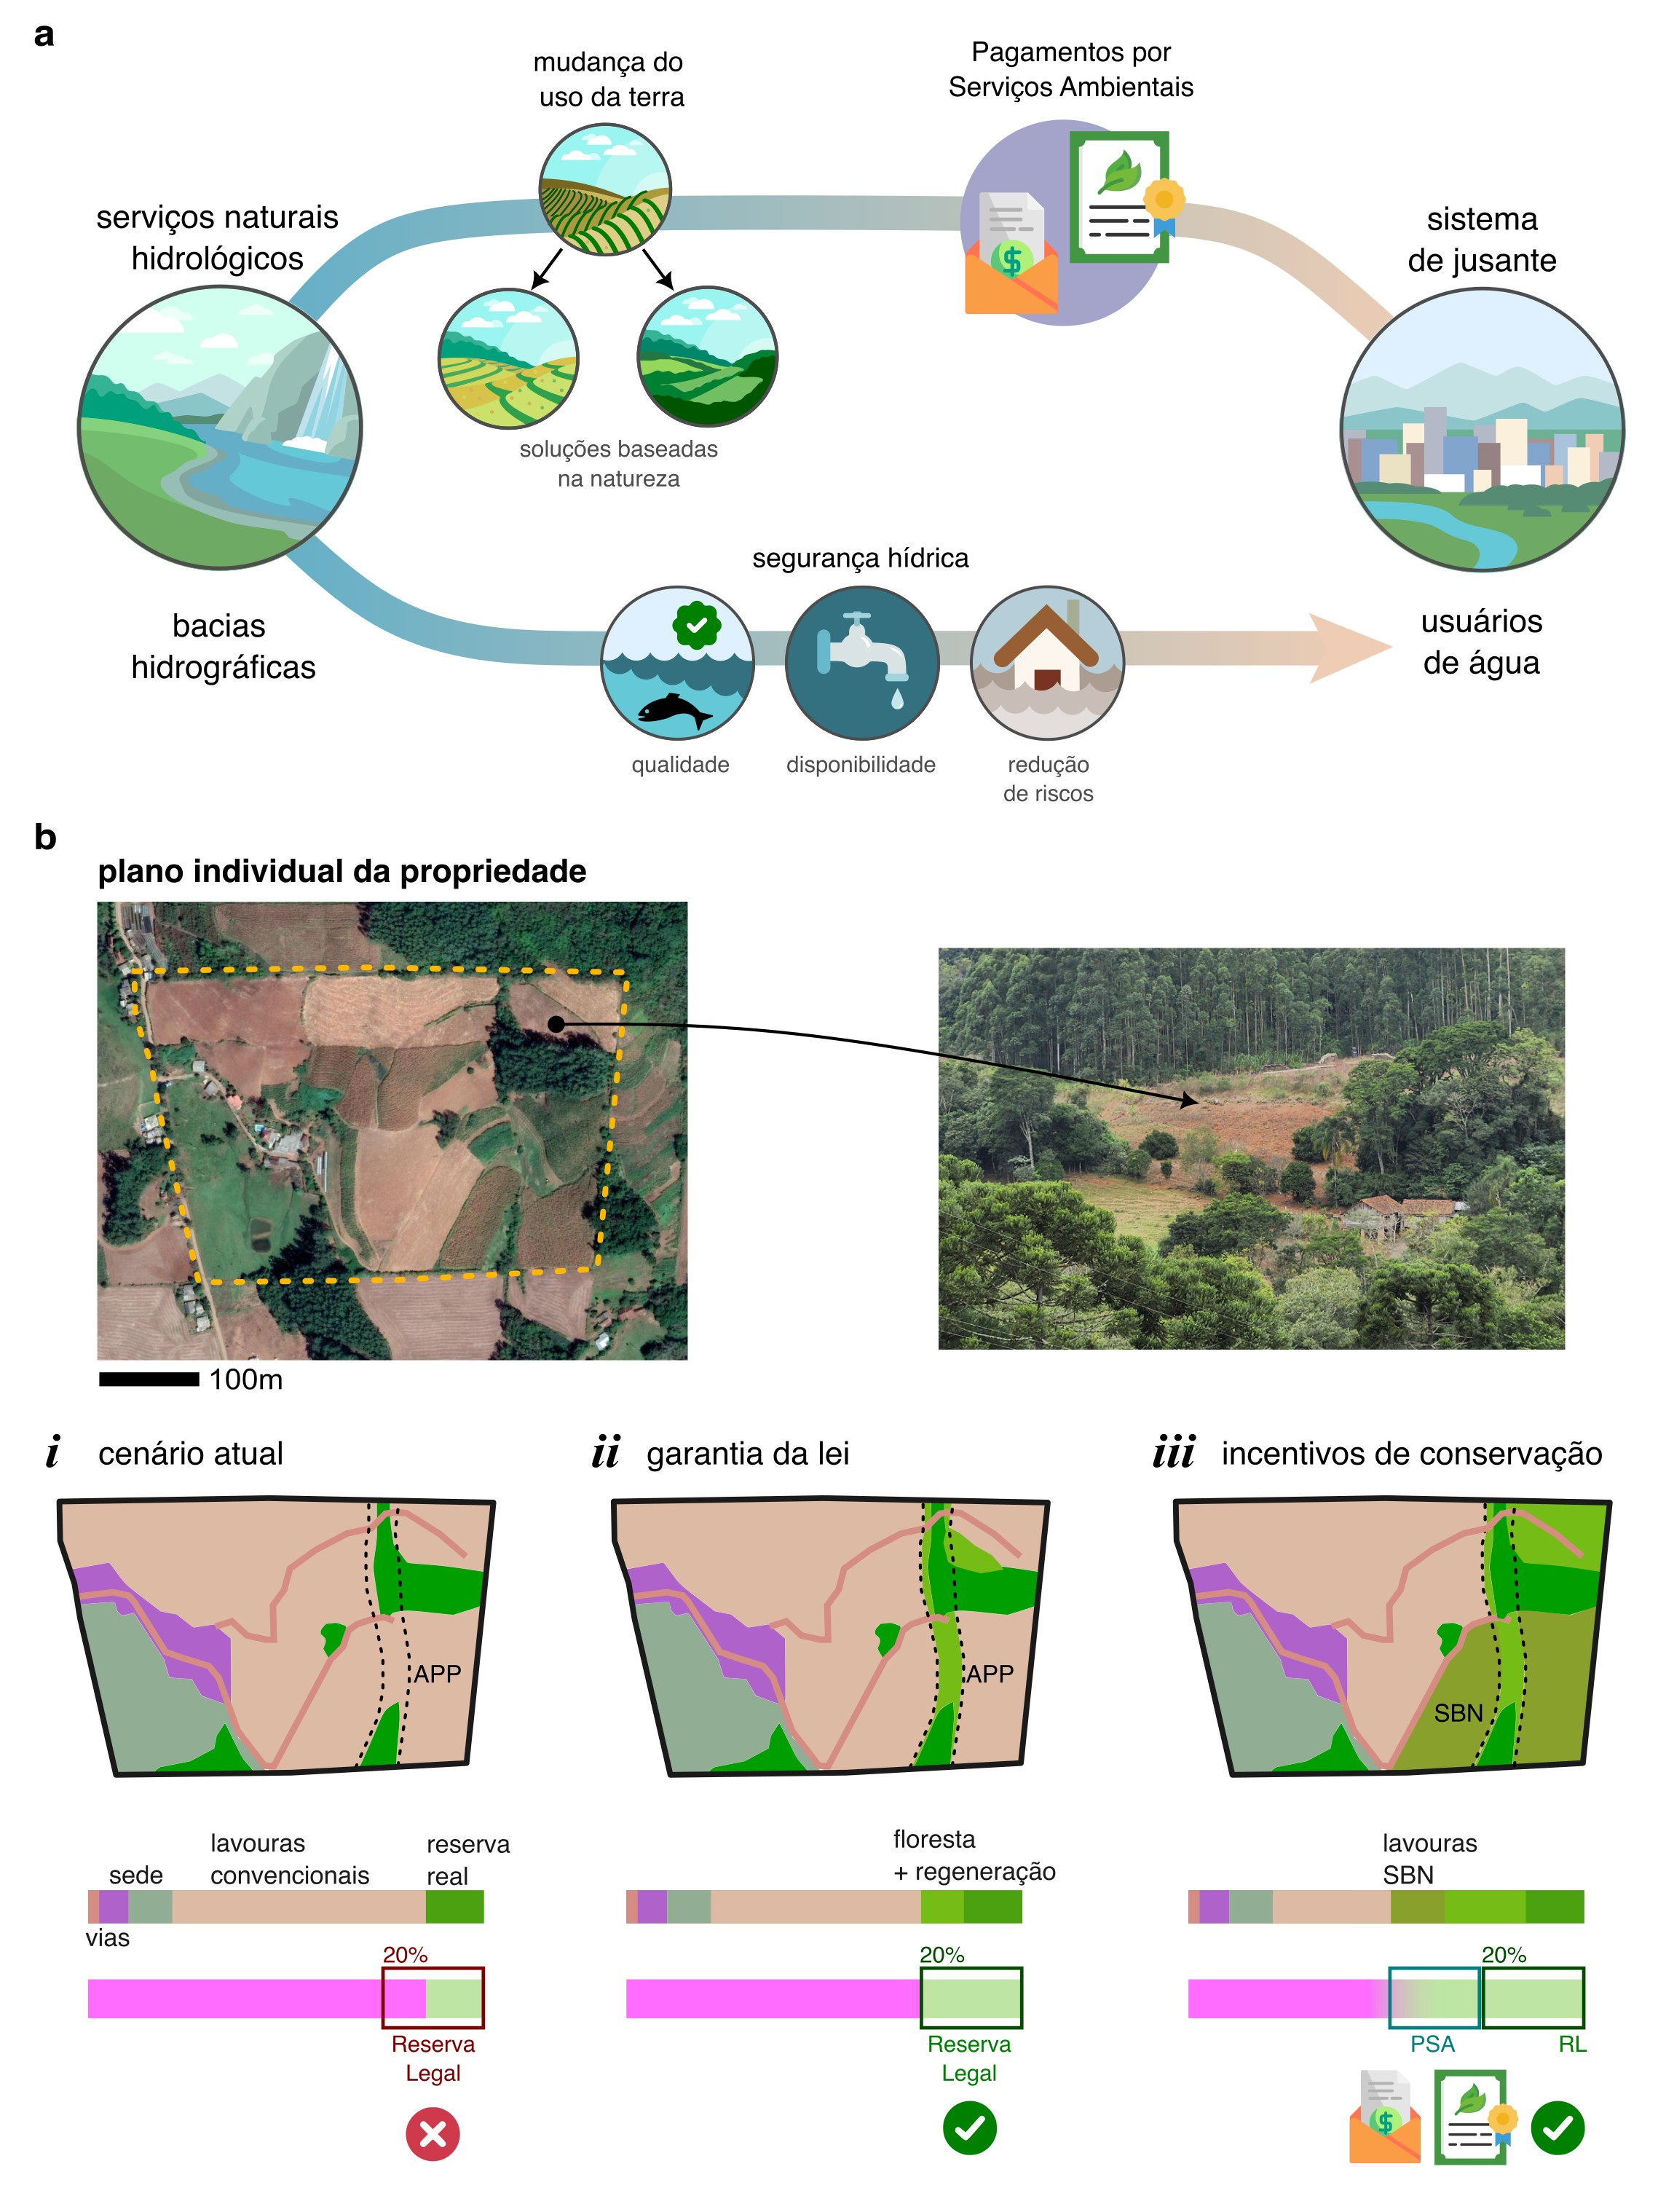
\includegraphics[width=0.98\linewidth]{figs/fig_pes.jpg}		
\caption[Os esquemas de Pagamentos por Serviços Ambientais]
{\textbf{---\;Os esquemas de Pagamentos por Serviços Ambientais (PSA) em bacias hidrográficas.}     
    \;\textbf{a}\;---\;Os esquemas de PSA hídricos são instrumentos econômicos que estabelecem, na prática, contratos de arrendamento para a conservação da terra em bacias de ordem zero. Essa é uma estratégia que objetiva induzir uma mudança de comportamento dos proprietários de terra para além das obrigações legais, retornando incrementos de segurança hídrica para o usuários de água de jusante.
    \;\textbf{b}\;---\;No Brasil, o Plano Individual da Propriedade (PIP), que resulta do Cadastro Ambiental Rural, fornece os meios técnicos de operacionalizar o PSA hídrico. No exemplo, a propriedade encontra-se em inconformidade para com o Novo Código Florestal (detalhe \textrm{\textit{i}}), que exige uma Reserva Legal de 20\% da área do imóvel na maior parte dos biomas (detalhe \textrm{\textit{ii}}). O PSA, assim, vai além do obrigatório, incentivando o proprietário a expandir a infraestrutura verde, seja pela restauração ecológica, seja por práticas de manejo do solo (detalhe \textrm{\textit{iii}}).
}
\label{fig:eco:pes} 		
\end{figure}

\par Os esquemas de \acrfull{pes}\footnote{Nomenclatura amplamente utilizada no Brasil, conforme a Política Nacional. Na literatura internacional, usa-se o termo \textit{Payments for Ecosystem Services}.} constituem instrumentos econômicos de gestão ambiental que incentivam o uso sustentável dos serviços naturais. No contexto da gestão de bacias hidrográficas, eles são conhecidos como \say{\acrshort{pes} hídricos}\footnote{Tradução livre de \textit{Watershed PES}.}, promovendo mudanças no uso da terra, especialmente por meio da expansão de infraestrutura verde em bacias de ordem zero, nas áreas de cabeceiras. O instrumento de \acrfull{pes} hídrico pode ser entendido como a formalização de \textbf{arrendamentos para conservação}, acordos que mantêm a propriedade privada da terra, mas transferem o direito de uso dela para a conservação dos recursos naturais por um período determinado, renovável conforme o contrato. A negociação do direito de uso da terra pode variar, desde a proibição total em áreas muito sensíveis até a implementação de práticas de manejo sustentável, cabendo à instituição pagadora monitorar o cumprimento das condições, tanto pelos proprietários atuais quanto pelos futuros. Nesse âmbito, a terra em si deve ser compreendida sob o conceito de \textbf{terra ricardiana}, que consiste nas características indestrutíveis e inesgotáveis que a superfície oferece para as atividades humanas se desenvolverem \cite{haddad2023}. A terra ricardiana geralmente não é um recurso comum, pois costuma ser parcelada em lotes exclusivos entre os agentes econômicos, principalmente por propriedades privadas. Além disso, a terra ricardiana possui um valor de uso que não está associado somente à fertilidade do solo, mas também com suas condições de acesso e proximidade de \textit{outros} recursos. Por exemplo, em razão da sua localização, um hectare de terra no perímetro urbano de uma cidade tem um valor de uso relativamente maior que um hectare no interior rural. Mas o uso da terra frequentemente gera externalidades negativas que degradam diversos serviços naturais comuns, incluindo os serviços naturais hidrológicos. Um exemplo disso é a função ambiental de armazenamento de água exercida pelas zonas vadosa e freática do solo, prolongando o escoamento de base nos rios durante as estiagens, um serviço essencial para a segurança hídrica. Esse serviço é severamente degradado pela compactação ou impermeabilização do solo tanto pelas atividades rurais como urbanas. Assim, como em outras questões envolvendo recursos comuns, os esquemas de \acrshort{pes} objetivam induzir os agentes econômicos que utilizam a terra a neutralizarem as externalidades negativas que geram ou mesmo produzir externalidade positivas.

\par Esse instrumento de gestão, de forma geral, classifica-se em três categorias principais, com base nos agentes financiadores e no tipo de incentivo econômico envolvido \cite{Smith2006a, Salzman2018a}. Pelo aspecto do financiamento, a primeira categoria são os \textbf{esquemas de \acrshort{pes} financiados por usuários}, que envolve os beneficiários diretos dos serviços naturais hidrológicos. Esses usuários podem ser indivíduos, empresas, ONGs ou atores públicos que se beneficiam diretamente da conservação, melhoria ou reestabelecimento dos serviços naturais. Um exemplo típico são os incentivos pagos por companhias hidrelétricas e de saneamento aos proprietários de terra nas regiões a montante, situação que faz das companhias um agente intermediário entre os consumidores finais e os produtores iniciais dos serviços naturais \cite{Fuentes-Llanillo2021}. Já os \textbf{esquemas de \acrshort{pes} financiados por terceiros} envolvem agentes econômicos que atuam em nome dos beneficiários. Nesse caso, o comprador é uma entidade pública ou privada, como organizações de conservação ou agências de governo, que não utilizam diretamente os serviços naturais. Programas governamentais de redução de desmatamento e incentivo ao reflorestamento, especialmente na China, são exemplos dessa modalidade. Por fim, os \textbf{esquemas \acrshort{pes} financiados por regulações} abrangem incentivos pagos por agentes econômicos que precisam cumprir obrigações regulatórias, compensando externalidades causadas em outros locais. Esquemas desse tipo, ao gerar demanda por compensações no formato \textit{cap-and-trade}, favorecendo um mercado de \textbf{créditos ambientais}, requerem o advento de instituições responsáveis por centralizar e gerir essas informações em um banco. Pelo aspecto dos incentivos econômicos, as categorias dividem-se em \textbf{incentivos econômicos diretos} e \textbf{incentivos econômicos indiretos}. O primeiro caso envolve o pagamento em si, quando os agentes econômicos recebem um valor em moeda corrente pelo arrendamento da conservação. O segundo caso envolve tanto \textbf{ajuda de custeio} na instalação da infraestrutura verde, incluindo atividades de extensão rural, quanto a \textbf{certificação ecológica}, um rótulo que agrega valor de mercado na produção dos agentes econômicos. É claro que essas classes não são monolíticas, mas difusas, sendo possíveis mesclas e sobreposições entre as abordagens. No caso dos esquemas de \acrshort{pes} hídrico, seja qual for o formato principal de financiamento e incentivo, a experiência aponta que os esquemas de \acrshort{pes}, para saírem do papel, precisam se organizar em torno de um programa socio-ambiental abrangente, que envolve diversas instituições parceiras e outros objetivos de desenvolvimento sustentável \cite{Viani2019a}. Por exemplo, Richards \textit{et al.} (2015) \cite{Richards1931a} ilustram que o programa de \acrshort{pes} \say{Conservador das Águas}, em Extrema (MG), para ser efetivado contou com uma articulação de múltiplas organizações financiadoras e apoiadoras, incluindo desde prefeituras, governos estaduais, agências e comitês de bacia até ONGs conservacionistas, entidades de extensão rural, entidades de ensino e de pesquisa.   

\par Nesse rumo, cabe ressaltar que os instrumentos econômicos não são substitutos de medidas de comando e controle, mas sobrepostos. Assim, os esquemas de \acrshort{pes} objetivam \textit{incrementar} a conservação dos serviços naturais para além das obrigações impostas por lei. No Brasil, a principal regulação do uso da terra em escala nacional consiste na \textbf{Lei Federal de Proteção da Vegetação Nativa}, chamada informalmente de \textbf{Novo Código Florestal} (apesar da vegetação nativa no Brasil incluir outras formações vegetais). \cite{brasil12651}. Outras regulações relevantes na escala nacional, mas não uniformes, são o Estatuto das Cidades \cite{brasil2021}, que oferece aos municípios poder regulatório do uso da terra pelo Plano Diretor, e o Sistema Nacional de Unidades de Conservação \cite{Brasil2000}, que permite aos membros da federação criarem e regularem áreas protegidas. Quando aprovado em 2012, ao revisar a lei anterior, o Novo Código Florestal introduziu ferramentas cadastrais como o \textbf{Cadastro Ambiental Rural (CAR)} e diretrizes de compensação do desmatamento, que favorecem o estabelecimento de esquemas de \acrshort{pes}. Essas iniciativas são ainda mais necessárias diante das mudanças problemáticas trazidas pela nova legislação. Conforme Soares-Filho \textit{et al.} (2014) \cite{Soares-filho2014a}, a revisão concedeu anistia a desmatadores ilegais, o que pode comprometer a conservação em propriedades privadas, onde encontra-se 53\% da vegetação nativa do Brasil. Além disso, Brancalion \textit{et al.} (2016) \cite{Brancalion2016a} ressaltam que a flexibilização de exigências para recuperação ambiental e a manutenção de atividades agropecuárias em áreas protegidas enfraqueceram a proteção obrigatória do solo e dos recursos hídricos, aumentando o risco de perda dos serviços naturais. Nesse contexto, os esquemas de \acrshort{pes} surgem como um complemento relevante às regulamentações legais, oferecendo incentivos financeiros para os proprietários de terra se comprometerem voluntariamente com práticas conservacionistas. 

\par Em síntese, a Lei Federal de Proteção da Vegetação Nativa institui no Brasil as regras para o zoneamento ambiental das propriedades privadas, produzindo assim o \textbf{Plano Individual da Propriedade (PIP)}. Além de zonas opcionais como as glebas de cultivo, área de pousio, servidões de acesso, sede da propriedade, etc, o PIP possui duas zonas obrigatórias, que são a \textbf{Reserva Legal (RL)} e as \textbf{Áreas de Proteção Permanente (APP)}. A Reserva Legal, consiste na zona de vegetação nativa obrigatória que cada lote deve apresentar, calculada por uma fração da área total. Em outras palavras, ela define a extensão máxima das atividades econômicas que não fazem uso da vegetação nativa diretamente, como a agricultura. A proporção dessa zona varia conforme a região. Na Amazônia Legal, a fração de RL deve ser de 85\% em áreas de floresta, 35\% em áreas de cerrado e 20\% em áreas de campos gerais. No resto do País, a fração de RL é de 20\%, uma fração questionável em termos de sustentabilidade, a depender do uso da terra nos outros 80\%. Pelo ponto de vista ecológico, Banks-Leite \textit{et al.} (2014) \cite{Banks-leite2014a} apontam que, no bioma da Mata Atlântica, o limite viável para a conservação das comunidades de vertebrados é de aproximadamente 40\% de habitat natural. Do lado hidrológico, Caldwell \textit{et al.} (2023) \cite{Caldwell2023} demonstram que uma taxa de 20\% de cobertura florestal pode implicar um decaimento da qualidade de água em até uma ordem de magnitude (10 vezes pior) do que em bacias completamente conservadas. Além disso, de acordo com a lei, a RL pode ser explorada economicamente com manejo sustentável, e, caso não haja vegetação suficiente no lote, o proprietário pode recuperar a área ou compensá-la em outra propriedade, desde que seja no mesmo bioma. As Áreas de Proteção Permanente, por outro lado, são áreas que, mesmo sem vegetação nativa, devem ser preservadas para proteger recursos hídricos, biodiversidade, solo e a estabilidade das encostas. Elas incluem nascentes, encostas íngremes, topos de morro e cursos d'água, entre outros, formando zonas de tamponamento nas áreas ripárias com larguras definidas conforme o porte do curso d'água. Pela lei, as APPs podem ser contabilizadas no percentual de Reserva Legal, ainda que elas sejam obrigatórias mesmo que esse percentual seja excedido. Por exemplo, se um lote apresenta mais de 20\% de encostas muito íngremes, a área total de APP deve se expandir para proteger essas encostas.

\par Embora o \acrshort{pes} seja uma ferramenta relevante para definir os limites econômicos às atividades humanas em uma bacia hidrográfica, ele não é a única solução. Uma alternativa possível, e mais robusta, é simplesmente obrigar os proprietários a seguirem normas mais rígidas de uso da terra, pela imposição da lei. Em um cenário extremo, os agentes econômicos interessados na preservação dos serviços naturais hidrológicos adquirem a exclusividade do uso da terra na bacia, eliminando a necessidade de negociações com outros agentes. Esse cenário se observa, em grande parte, no nordeste dos Estados Unidos, uma região onde há alta demanda por água para abastecimento de grandes cidades, como Nova Iorque e Boston \cite{alcott2013}. Nessa região, as companhias de saneamento, privadas e governamentais, obtiveram a exclusividade de áreas críticas para os mananciais pela compra direta dos imóveis rurais. Nesse sentido, o estudo de caso de Nova Iorque nas bacias de Catskills e Delaware recebe uma dose de críticas da parte de Blanchard \textit{et al.} (2015) \cite{Blanchard2015a}, principalmente por ter-se tornado uma narrativa favorável aos incentivos econômicos, mas que na realidade se fundamentou substancialmente no comando e controle, além de ter feitos investimentos mais pesados em saneamento rural (infraestrutura cinza) do que na recuperação de florestas (infraestrutura verde). Uma estratégia semelhante ocorre com o zoneamento de áreas protegidas, chamadas no Brasil de \textbf{Unidades de Conservação de Proteção Integral}, como Estações Ecológicas ou Parques Naturais. Nesse caso, a terra passa a ser de uso exclusivo do Estado, com a devida indenização aos antigos proprietários, seja em âmbito municipal, estadual ou federal. Uma alternativa intermediária no Brasil é a criação de \textbf{Unidades de Conservação de Uso Sustentável}, como as Áreas de Proteção Ambiental (APA), nas quais a propriedade privada da terra é mantida, mas o seu uso é disciplinado pelo \textbf{Plano de Manejo} da unidade. Em áreas de mananciais, por exemplo, as práticas de agricultura convencional com o uso de agrotóxicos, pode ser proibida. Os \textbf{Planos Diretores} municipais também podem exercer esse papel intermediário, regulando as atividades permitidas em áreas de manancial, como é o caso do Parque Municipal da Lagoa do Peri, em Florianópolis, uma área que os imóveis rurais existentes são sujeitas a uma regulação do solo mais rigorosa.

\subsection{Diretrizes de planejamento}

{\renewcommand{\arraystretch}{1.5}
\begin{table}[t!]
    \centering	
    \tiny
    \sffamily
    \rowcolors{2}{white}{rowgray}
    \begin{tabular}{ 
         >{\raggedright\arraybackslash}m{1.5cm}  
         >{\raggedright\arraybackslash}m{2.2cm}  
         >{\raggedright\arraybackslash}m{4.6cm}
         >{\raggedright\arraybackslash}m{4.6cm}
    }
    \toprule 
\textbf{Princípio} & \textbf{Objetivo} & \textbf{Diretrizes científicas básicas} & \textbf{Diretrizes científicas desejáveis} \\
\midrule
\textbf{Métricas}& 
Métodos robustos, eficientes e versáteis para obtenção de dados.
& \begin{itemize}
    \setlength{\itemsep}{-0.4em}
    \item Devem ser relevantes, confiáveis e adequados em escala.
    \item Devem cumprir com normas voluntárias, certificações e regulamentos.
    \item Devem refletir escalas espaço-temporais, como identificado em Dinâmica.
    \item Otimizar o equilíbrio entre precisão e simplicidade.
    \item Avaliar o progresso (em conjunto com Linha de Base e Monitoramento).
    \item Estabelecer benchmarks (em conjunto com Linha de Base e Monitoramento).
    \item Medir tanto mudanças absolutas quanto mudanças nas tendências. 
\end{itemize}
& \begin{itemize}
    \setlength{\itemsep}{-0.4em}
    \item Preferencialmente selecionadas para permitir comparações entre tipos de serviços.
    \item Avaliar como os serviços influenciam uns aos outros.
\end{itemize} \\
\textbf{Linha de base}
& Documentar as condições iniciais e de referência. 
& \begin{itemize}
    \setlength{\itemsep}{-0.4em}
    \item Medir as influências das intervenções nos serviços.
    \item Medir o status e as tendências dos serviços não-alvo.
    \item Garantir que as medições sejam viáveis, dado os recursos.
\end{itemize}
& \begin{itemize}
    \setlength{\itemsep}{-0.4em}
    \item Avaliar o estado inicial das ameaças exógenas e endógenas aos serviços.
    \item Medir fatores importantes para prever tendências dos serviços.
\end{itemize} \\
\textbf{Monitoramento}
& Acompanhar fatores necessários para gestão, negociações, avaliações e previsões.
& \begin{itemize}
    \setlength{\itemsep}{-0.4em}
    \item Quantificar benefícios associados aos serviços-alvo.
    \item Identificar escalas espaço-temporais antes da implementação.
    \item Usar métodos/protocolos estabelecidos e melhores práticas para monitoramento.
    \item O monitoramento deve informar a tomada de decisões.
    \item O monitoramento deve detectar mudanças potenciais nas condições de linha de base.
\end{itemize}
& \begin{itemize}
    \setlength{\itemsep}{-0.4em}
    \item Monitorar serviços não-alvo que influenciam os serviços-alvo.
\end{itemize} \\
\textbf{Dinâmica}
& Garantir a capacidade do projeto para se adaptar a processos naturais e humanos dinâmicos. 
& \begin{itemize}
    \setlength{\itemsep}{-0.4em}
    \item Identificar serviços naturais chave para cada classe de serviço além dos serviços-alvo.
    \item Identificar escalas espaço-temporais dos serviços-alvo.
    \item Identificar necessidades de dados, recursos e lacunas.
    \item Identificar estressores e sua variabilidade espaço-temporal.
    \item Identificar e prever tendências de ameaças endógenas e exógenas.
\end{itemize} 
& \begin{itemize}
    \setlength{\itemsep}{-0.4em}
    \item Determinar como a diversidade funcional influencia a resiliência. \item Identificar funções de produção dos serviços e suas sensibilidades.
    \item Determinar trade-offs e sinergias entre os serviços.
\end{itemize} \\ 
\textbf{Múltiplos serviços} 
& Reconhecer trade-offs e sinergias entre serviços. 
& 
& \begin{itemize}
    \setlength{\itemsep}{-0.4em}
    \item Avaliar como a intervenção influencia os outros serviços.
    \item Evitar contagem dupla de serviços.
    \item Avaliar impactos da intervenção sobre serviços não-alvo.
\end{itemize} \\
\textbf{Sustentabilidade} 
& Garantir durabilidade e sustentabilidade do projeto. 
& 
& \begin{itemize}
    \setlength{\itemsep}{-0.4em}
    \item Estimar desempenho de curto e longo prazo do projeto ou programa.
\end{itemize} \\
\bottomrule
\end{tabular}
\caption[Princípios e diretrizes científicas para programas de \acrshort{pes}]{
        \textbf{Princípios, objetivos e diretrizes científicas para programas de \acrshort{pes}}\; --- \;Relação esquematizada por Naeem \textit{et al.} (2015) \cite{Naeem2015b}}
    \label{tbl:guidelines}

\end{table}
}

\par Ao longo das últimas duas décadas, a literatura acadêmica e técnica, a partir de experiências tanto teóricas quanto práticas, debateu extensamente as estrutura básica que um esquema de \acrshort{pes} em bacias hidrográficas deve oferecer para ser considerado uma estratégia bem-sucedida. Ainda na esteira do relatório da Avaliação Ecossistêmica do Milênio, o relatório de Smith \textit{et al.} (2006) \cite{Smith2006a}, uma iniciativa da \textit{International Union for Conservation of Nature} (IUCN), trouxe um arcabouço conceitual e prático pioneiro e abrangente para a instalação de esquemas de \acrshort{pes} em bacias hidrográficas. Entre as principais contribuições, uma delas foi a própria nomenclatura de \say{serviços naturais hidrológicos}, catalogados na Tabela \ref{tbl:waterserv}. Mas além disso, Smith \textit{et al.} (2006) enfatizam que, para serem efetivos, os esquemas de \acrshort{pes} devem se fundamentar em evidências o mais sólidas possíveis. As ações desenvolvidas, portanto, devem resultar em benefícios identificáveis para os usuários, com relações claras entre o uso da terra a montante e os serviços naturais hidrológicos para os usuários a jusante.

\par Entre as diretrizes de Smith \textit{et al.} (2006), destaca-se a necessidade de se estimar a \textbf{capacidade de oferta dos serviços naturais}, isto é, o quanto deve-se esperar de mudanças nos processos biofísicos de montante e, consequentemente, no valor econômico para jusante. Em síntese, os autores defendem que se busque mensurar os dois extremos do modelo de cascata de Haines-Young \& Potschin -- processos e valor. Assim, o desempenho do \textbf{serviço-alvo} deve ser estimado por meio de indicadores de processos específicos, consensuais e mensuráveis, permitindo tanto a definição clara de prioridades de ações quanto um acompanhamento contínuo e alinhado com as metas do programa. Nessa linha, sugere-se a adoção de \textbf{indicadores de estado}, que revelam a situação observada dos processos subjacentes aos serviços, e \textbf{indicadores de uso sustentável}, que revelam o quanto se está acima ou abaixo do limite econômico do uso desse recurso. Exemplos desses indicadores também estão listados na Tabela \ref{tbl:waterserv}. No que se refere à valoração, Smith \textit{et al.} (2006) apontam que os esforços de valoração econômica devem se concentrar na \textbf{análise de custo-benefício} entre as partes envolvidas. O custo corresponde aos incentivos econômicos oferecidos pela entidade pagadora, negociado diretamente com os agentes econômicos. Idealmente, esse custo deve ser inferior aos benefícios econômicos estimados com métodos de valoração pela melhoria dos serviços naturais proporcionados, justificando, assim, o investimento no esquema de pagamento. 

\par As diretrizes propostas por Smith \textit{et al.} (2006) sinalizaram para uma ampla discussão sobre o assunto, com diversos autores contribuindo sobre diferentes aspectos. Nesse sentido, a contribuição de Luca Tacconi (2012) \cite{Tacconi2012a}, buscou unificar conceitos importantes para o tema, revisando as problemáticas e atributos que definem um esquema de \acrshort{pes} bem-sucedido. O autor aponta para três princípios essenciais a serem observados: a adicionalidade, a condicionalidade e a transparência. O \textbf{princípio da adicionalidade} objetiva assegurar que os incentivos econômicos produzam benefícios que não ocorreriam \textit{sem} o esquema de \acrshort{pes}. Sendo fundamental na aplicação de modelos hidrológicos, esse princípio será aprofundado na próxima seção. O \textbf{princípio da condicionalidade}, por sua vez, preconiza que os pagamentos em um esquema de \acrshort{pes} estejam diretamente ligados ao cumprimento de práticas que assegurem a provisão de serviços naturais. Ou seja: os contratos de arrendamento para conservação devem ser cumpridos pelas partes contratadas. Isso implica, portanto, que exista alguma forma de fiscalização periódica do uso da terra que condiciona a continuidade do contrato. Se um proprietário decide promover uma grande queimada em seu lote, por exemplo, o seu contrato de \acrshort{pes} deve ser rescindido e os pagamentos suspensos. Embora a aplicação rigorosa desse princípio possa aumentar os custos indiretos do financiamento do programa e afetar a motivação voluntária dos agentes econômicos, sua completa ausência pode comprometer a efetividade do esquema, arriscando desperdício de recursos sem a garantia de resultados ambientais reais. Por fim, o \textbf{princípio da transparência} envolve a disponibilização clara e confiável de informações a todas as partes envolvidas, sendo essencial para a aceitação e a integridade dos esquemas de \acrshort{pes}. Tacconi ressalta que baixos níveis de transparência, tanto nas negociações quanto na definição de valores dos pagamentos, podem gerar desconfiança e percepção de corrupção, especialmente em contextos em que o financiamento é feito por terceiros, como no caso das compensações ambientais. A transparência é também vital para o sucesso do escalonamento do programa, pois está associada à confiança e à capacidade de verificação, componentes essenciais para a cooperação entre os envolvidos. Para tanto, recomenda-se a divulgação pública de informações sobre os critérios técnicos de seleção de áreas prioritárias, os procedimentos de escolha dos participantes, os métodos de valoração e a distribuição dos benefícios. Uma estratégia que ganhou tração para articular esse princípio, ilustrada por Young \& Bakker (2014) \cite{Young2014a}, são as \textbf{calculadoras de \acrshort{pes}}. Assim, a entidade pagadora instancia um sistema de pontuação que avalia diversos atributos dos lotes candidatos a receberem o pagamento e determina o seu valor de forma objetiva e transparente. O sistema, portanto, pode permitir que um proprietário aumente o seu valor de \acrshort{pes} ao cumprir mais exigências ambientais do que outros, ganhando mais pontos na calculadora. Por exemplo, se forem adotadas práticas de manejo conservacionista do solo, o produtor rural deve ganhar mais incentivos do que em caso contrário.

\par O ciclo de diretrizes fundamentais se consolidou em grande medida pela publicação por Naeem \textit{et al.} (2015) \cite{Naeem2015b} do artigo \textit{Get the science right when paying for nature’s services}. Com a contribuição de dezenas de instituições técnicas e acadêmicas com experiências em centenas de estudos de caso, os autores propõem um conjunto estruturado de princípios e diretrizes científicas para fortalecer a integração da ciência nos esquemas de \acrshort{pes}, visando aumentar sua eficácia e garantir que gerem benefícios ambientais e sociais consistentes. Os princípios, listados na Tabela \ref{tbl:guidelines}, incluem a definição de métricas robustas, a documentação da linha de base, o monitoramento contínuo, a gestão dinâmica, a avaliação de múltiplos serviços, além de uma perspectiva de longo prazo. Cada princípio possui diretrizes básicas e desejáveis: por exemplo, o princípio das métricas orienta a seleção de métodos que equilibrem precisão e simplicidade, enquanto o monitoramento contínuo é essencial para rastrear benefícios e adaptar o manejo de forma eficaz. O princípio da dinâmica enfatiza a gestão adaptativa, atenta a processos naturais e humanos em curso e identificando mudanças de rota necessárias. O princípio dos múltiplos serviços busca reconhecer e gerenciar trade-offs e sinergias entre serviços naturais para além do serviço-alvo, evitando a contagem dupla e avaliando impactos em serviços não-alvo. O princípio da sustentabilidade, crucial para garantir a longevidade do projeto, incentiva uma avaliação do desempenho de curto e longo prazo. Esses princípios de Naeem \textit{et al.} (2015), evidentemente, não substituem a abordagem de Tacconi, pois possuem múltiplas conexões com a adicionalidade, condicionalidade e transparência. 

\subsection{O princípio da adicionalidade}

\begin{figure}[t!] 
\centering				
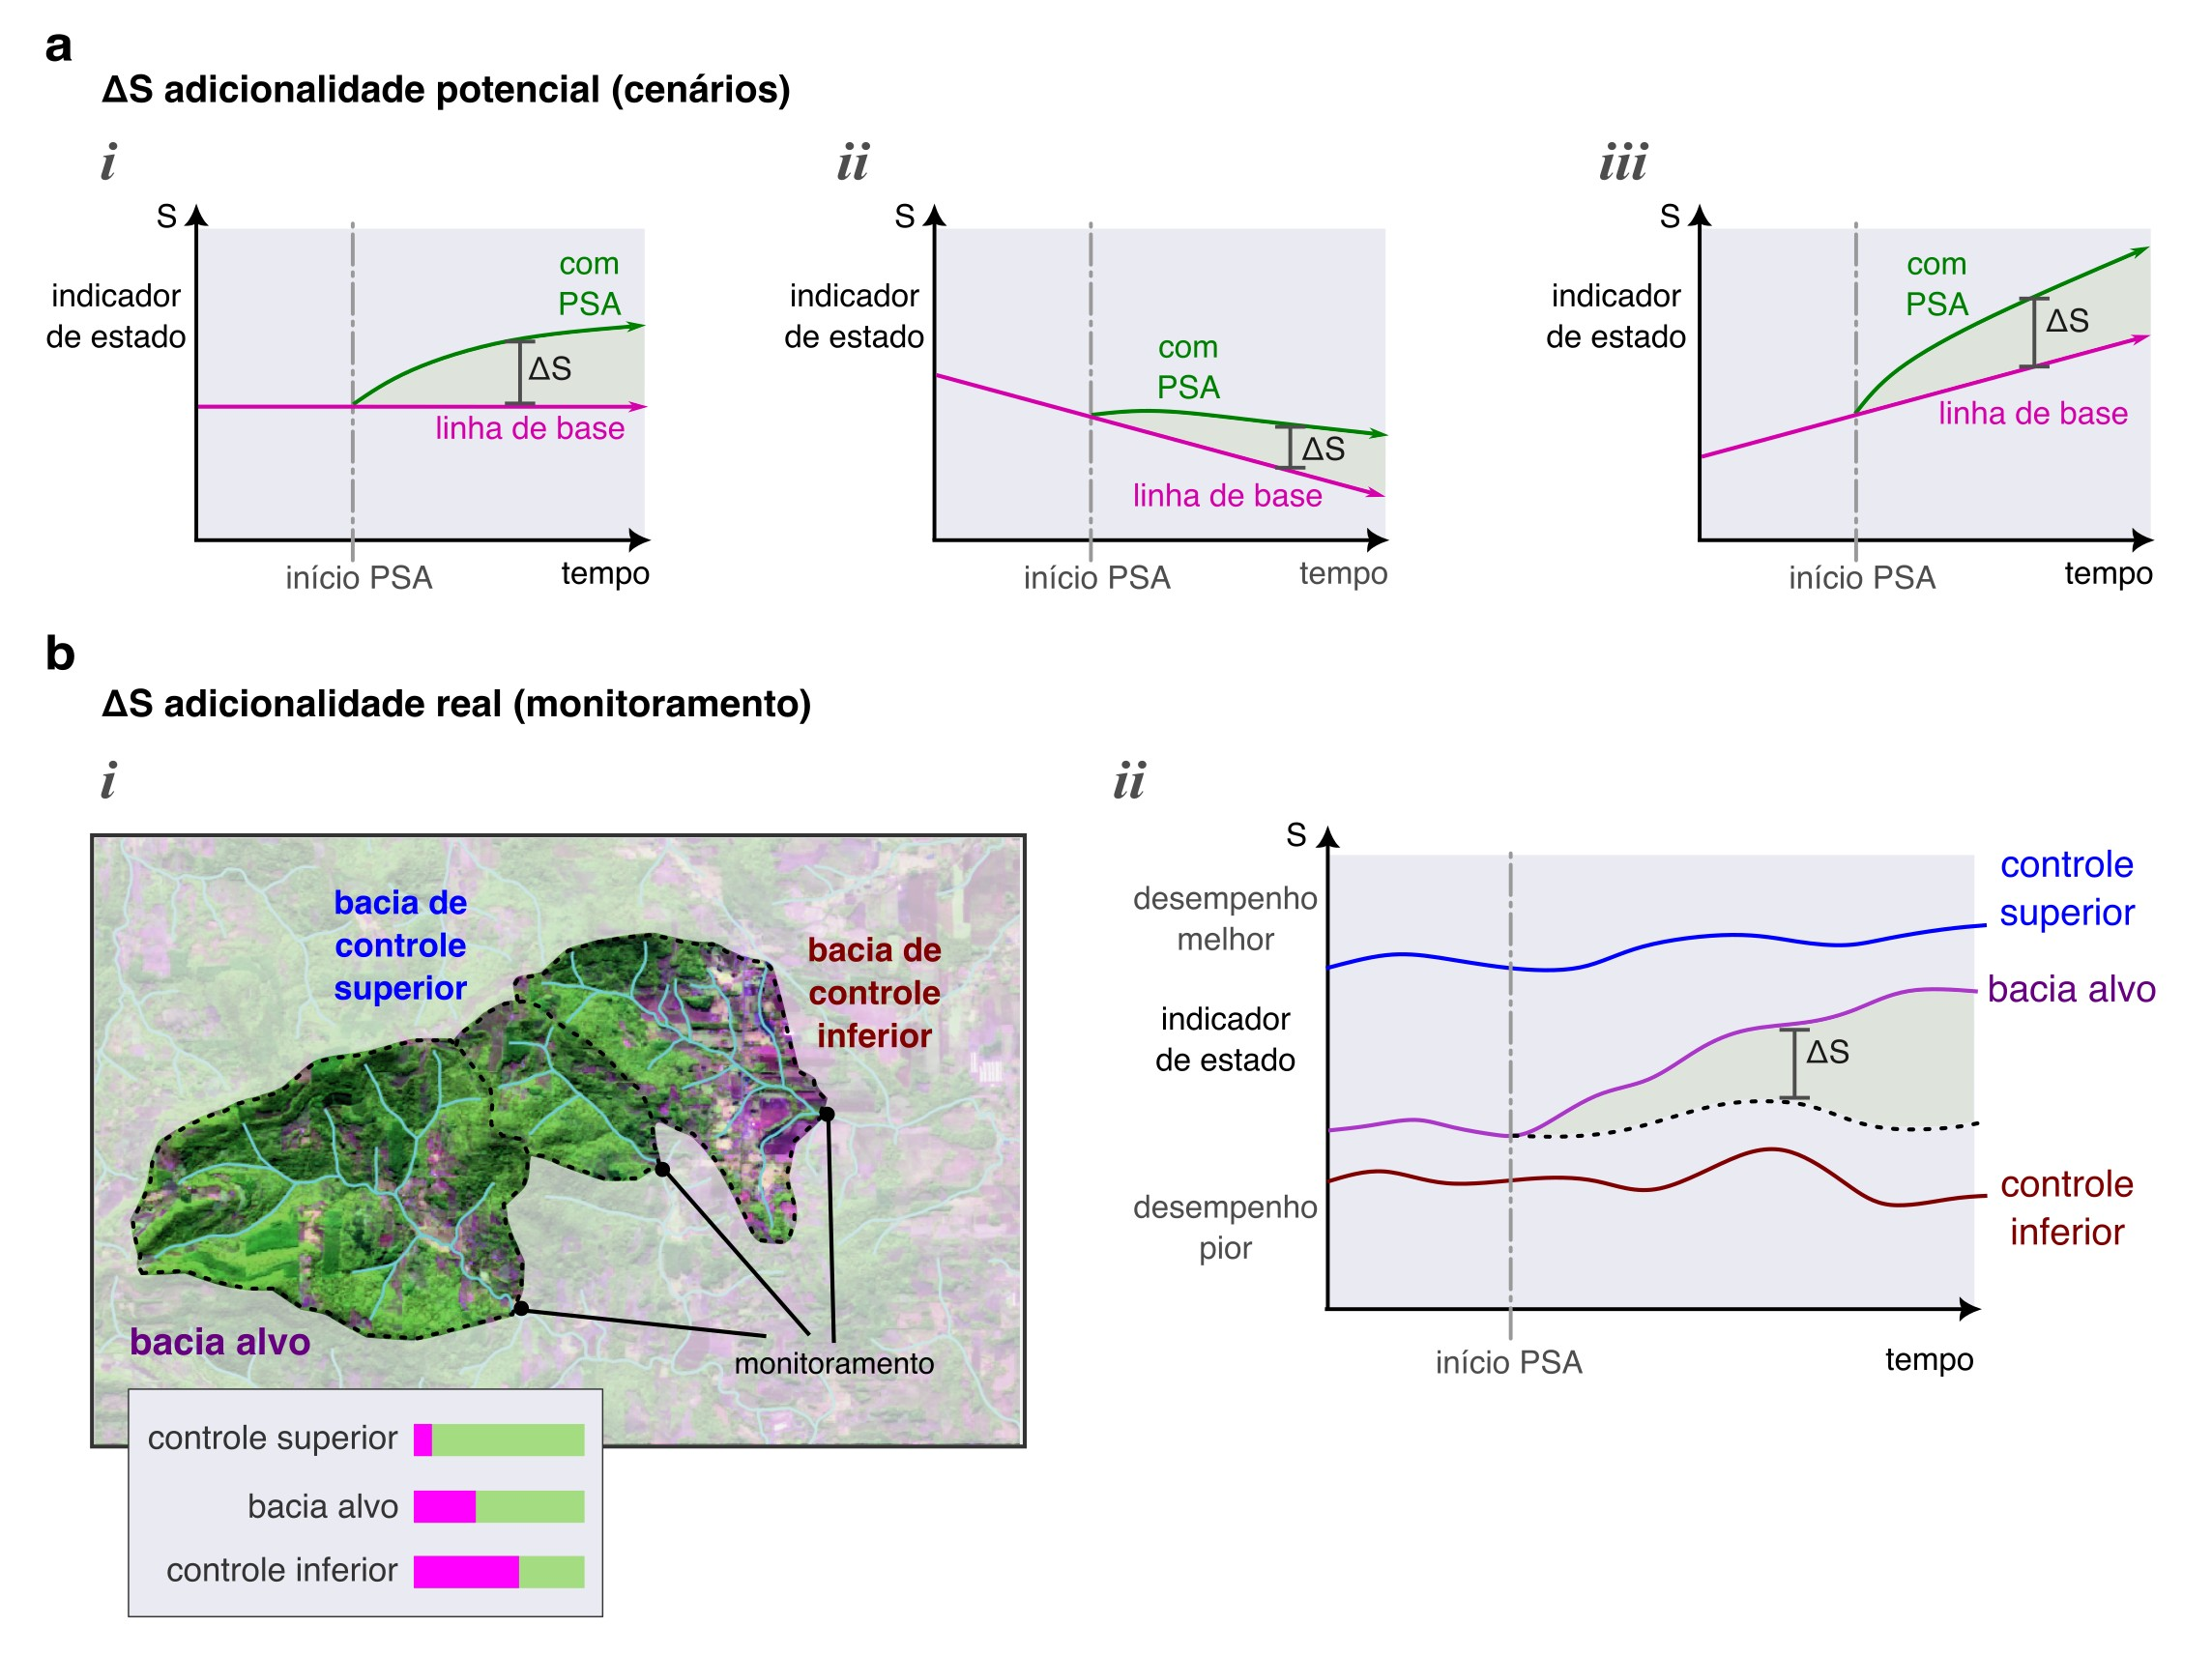
\includegraphics[width=0.98\linewidth]{figs/fig_add.jpg}		
\caption[Adicionalidade potencial e real.]
{\textbf{---\;Adicionalidade potencial e real.}
    O princípio da adicionalidade objetiva assegurar que os incentivos econômicos produzam benefícios que não ocorreriam sem o PSA.
    \;\textbf{a}\;---\;Na fase de planejamento de um esquema de PSA, deve-se buscar estimar a adicionalidade potencial $\Delta S$, calculada pela diferença entre um indicador de estado $S$ em cenários com e sem PSA. O cenários podem ser estacionários (detalhe \textrm{\textit{i}}), desfavoráveis (detalhe \textrm{\textit{ii}}) e favoráveis (detalhe \textrm{\textit{iii}}). O cenário sem PSA consiste em uma linha de base para a comparação. Na prática, uma abordagem consiste em comparar o cenário atual (sem PSA) com um cenário de vegetação nativa potencial (100\% de conservação). Avaliações desse tipo oferecem subsídios para análise de custo-benefício, acopladas com métodos de valoração.    
    \;\textbf{b}\;---\;Na fase de operação de um esquema de PSA, a adicionalidade real deve ser mensurada a partir de monitoramento. Em PSA hídricos, em particular, esforços devem ser feitos para isolar causalidade de variáveis exógenas. Por exemplo, bacias pareadas próximas à bacia alvo podem ser eleitas como controles (detalhe \textrm{\textit{i}}). Bacias mais degradadas, assim funcionam como um controle inferior, e bacias mais preservadas funcionam como um controle superior (detalhe \textrm{\textit{ii}}).    
}
\label{fig:eco:add} 		
\end{figure}

Como citado acima, o princípio da adicionalidade objetiva assegurar que os incentivos econômicos produzam benefícios que não ocorreriam \textit{sem} o \acrshort{pes}. Ainda que pareça evidente, isso não era o caso em muitos estudos de planejamento com a aplicação de modelos hidrológicos, como atesta a revisão de Lele (2009) \cite{Lele2009a}. O autor verificou a falta de um arcabouço metodológico comum, rigoroso e compartilhado entre os extremos de modelagem de processos e valoração, em especial a falta de avaliação diante de cenários alternativos de uso da terra. Fragilidades metodológicas desse tipo motivaram Sven Wunder (2005, 2007) \cite{Wunder2005a, Wunder2007a} a elaborar considerações pioneiras sobre esse princípio. Para observar a adicionalidade, portanto, deve-se avaliar indicadores dos serviços naturais em relação ao \textbf{cenário da linha de base}, que funciona como referência de comparação para se dimensionar a capacidade de oferta do serviço natural. Com isso, esse princípio pode favorecer a viabilidade de um esquema de \acrshort{pes} apesar de condições desfavoráveis em termos absolutos. Por exemplo, mesmo com a redução de chuvas em uma bacia devido às mudanças do clima, a expansão da infraestrutura verde eventualmente pode resultar em um cenário futuro menos pior. A adicionalidade é, portanto, a \textit{diferença} entre o indicador de estado em condições atuais e o indicador de estado em condições de referência:
\begin{linenomath*}
\begin{equation}
\label{eq:aditionality}
\Delta\text{S}_{t} = \text{S}_{t} - \text{S}_{t^*} \quad \; \forall t 
\end{equation}
\end{linenomath*}
\noindent Em que $\Delta\text{S}_{t}$ é a adicionalidade no tempo $t$; $\text{S}_{t}$ é o indicador de estado do serviço natural no tempo $t$, e; $\text{S}_{t^*}$ é o indicador de estado do serviço natural no tempo $t^*$, que é o tempo no cenário da linha de base. Dessa forma, estimar a \textbf{adicionalidade potencial} em estudos de planejamento é o primeiro passo para justificar a implantação de um esquema de \acrshort{pes}, além de fornecer a base para o mapeamento e ordenamento de \textbf{áreas prioritárias}. O segundo passo, proposto por Kroeger \textit{et al.} (2013, 2019) \cite{Kroeger2013a, Kroeger2019a}, consiste na integração com métodos de valoração para subsidiar as análises de custo-benefício e retorno do investimento. Nesse sentido, a exploração de cenários de futuro feita por mim em Possantti \& Marques (2022) \cite{Possantti2022a} demonstra que esse movimento analítico não é trivial, dependendo fortemente de hipóteses auxiliares, em especial para se estimar custos de expansão das \acrshort{nbs} e os custos evitados verificados à jusante (ver Destaque \ref{box:dp}, no Capítulo 2).

\par Nos esquemas de \acrshort{pes} hídrico, o uso dos modelos hidrológicos torna-se crucial para a estimativa da adicionalidade potencial, pois é preciso simular o desempenho hidrológico da bacia hidrográfica em cenários alternativos de condições de contorno, comparando os resultados com e sem as ações planejadas (por exemplo: Ullrich \& Volk, 2009; Carvalho-Santos \textit{et al.}, 2014; Martinez-Martinez \textit{et al.}, 2014; Daneshi \textit{et al.}, 2021 \cite{Ullrich2009a, Carvalho-santos2014a, Martinez-martinez2014a, Daneshi2021a}). Essa avaliação, porém, só é possível ao se aplicar modelos conceituais que permitem a representação explícita dos diversos processos hidrológicos nas bacias de ordem zero. Os modelos baseados em dados, independentemente de sua capacidade preditiva, não são aplicáveis nesse tipo de problema, pois não permitem a inferência dedutiva sobre os cenários. Existe, porém, uma decisão metodológica importante a ser tomada, que é a definição do cenário da linha de base. Dentro de uma lógica da restauração de serviços naturais, a estratégia proposta por Lima \textit{et al.} (2017) \cite{Lima2017} consiste em definir esse cenário a partir da \textbf{vegetação nativa potencial}, ou seja, um cenário de cobertura da terra que reproduza o desenvolvimento natural da vegetação, sem alterações antrópicas. Nessa linha, a adicionalidade potencial se equipara à \textbf{anomalia hidrológica}, pois remete ao distúrbio hidrológico da mudança de cobertura da terra causado pelas atividades antrópicas atuais, como agricultura e urbanização. Por um lado, essa abordagem é simples e potencialmente baseada em evidências, pois a distribuição posterior dos parâmetros hidrológicos relacionados com a vegetação nativa potencial é estimável em bacias hidrográficas com alto grau de preservação. Por outro, ela não oferece meios de estimar a adicionalidade de outras formas de cobertura da terra que buscam bons desempenhos hidrológicos, como as \acrshort{nbs}, mas que não apresentam parâmetros prontamente estimáveis com evidências empíricas.   

\par O princípio da adicionalidade, entretanto, não deve se restringir à fase de planejamento: ele deve estar presente também na operação e gestão contínua de um programa de \acrshort{pes}. Assim, além da adicionalidade potencial, é essencial estimar a \textbf{adicionalidade real} ao longo do tempo, possibilitando medidas de adaptação dinâmica e ajustes de direção. Portanto, é necessário estabelecer e monitorar indicadores de estado do serviço-alvo que evidenciem a adicionalidade real. Idealmente, esses indicadores são as próprias variáveis hidrológicas que representam os processos subjacentes, como o escoamento de base, mas também podem incluir métricas indiretas e complementares, tais como a cobertura e o uso do solo, que podem ser monitorados a um custo mais baixo por sensoriamento remoto. Um exemplo de monitoramento da adicionalidade real é apresentado em Sone \textit{et al.} (2019) \cite{Sone2019a}, onde os autores avaliaram se um programa de \acrshort{pes} hídrico na Bacia do Rio Guariroba, no Centro-Oeste do Brasil. No estudo, foram monitoradas a precipitação e a vazão entre 2012 e 2016, período em que práticas de conservação de solo e água, como a construção de terraços em nível e a recuperação da vegetação ripária, foram implementadas na bacia. Os resultados obtidos, aliados a análise de tendência de séries temporais, mostraram que, embora os registros de precipitação apresentassem uma tendência de redução (1 mm por mês), o fluxo do escoamento de base aumentou em 18 litros por segundo durante o período de monitoramento. Essas observações de campo, assim, reforçam que é preciso checar também não apenas indicadores do serviço-alvo, mas variáveis exógenas que produzem \textit{circunstâncias extenuantes}, como a precipitação. Se a precipitação tivesse \textit{aumentado} no período de monitoramento, Sone \textit{et al.} (2019) não teriam como afirmar com tanta certeza sobre a adicionalidade real das ações. Nessa questão, um sistema de monitoramento ideal em um \acrshort{pes} hídrico deve adotar uma abordagem de \textbf{bacias pareadas}, em que se monitoram também \textbf{bacias de controle} onde \textit{não} são feitas ações. Bacias de controle mais degradadas, assim, fornecem uma \textbf{linha de base real}, enquanto bacias de controle mais preservadas oferecem uma \textbf{linha de teto real}. Um sistema de monitoramento com essa envergadura naturalmente consome recursos financeiros do programa, o que incentiva a exploração de estratégias menos convencionais, como o uso de \textbf{bioindicadores} — algas, plâncton e invertebrados de ecossistemas lóticos. Esses organismos, por refletirem múltiplos aspectos da estrutura ecológica, podem ser amostrados periodicamente, fornecendo informações sobre o histórico recente das condições ambientais. Essa abordagem permite identificar mudanças no ecossistema de forma mais econômica e complementar às variáveis hidrológicas, oferecendo uma visão integrada do impacto das práticas de conservação ao longo do tempo. 

\subsection{Aplicações com o modelo \texttt{PLANS}}

\begin{figure}[t!] 
\centering				
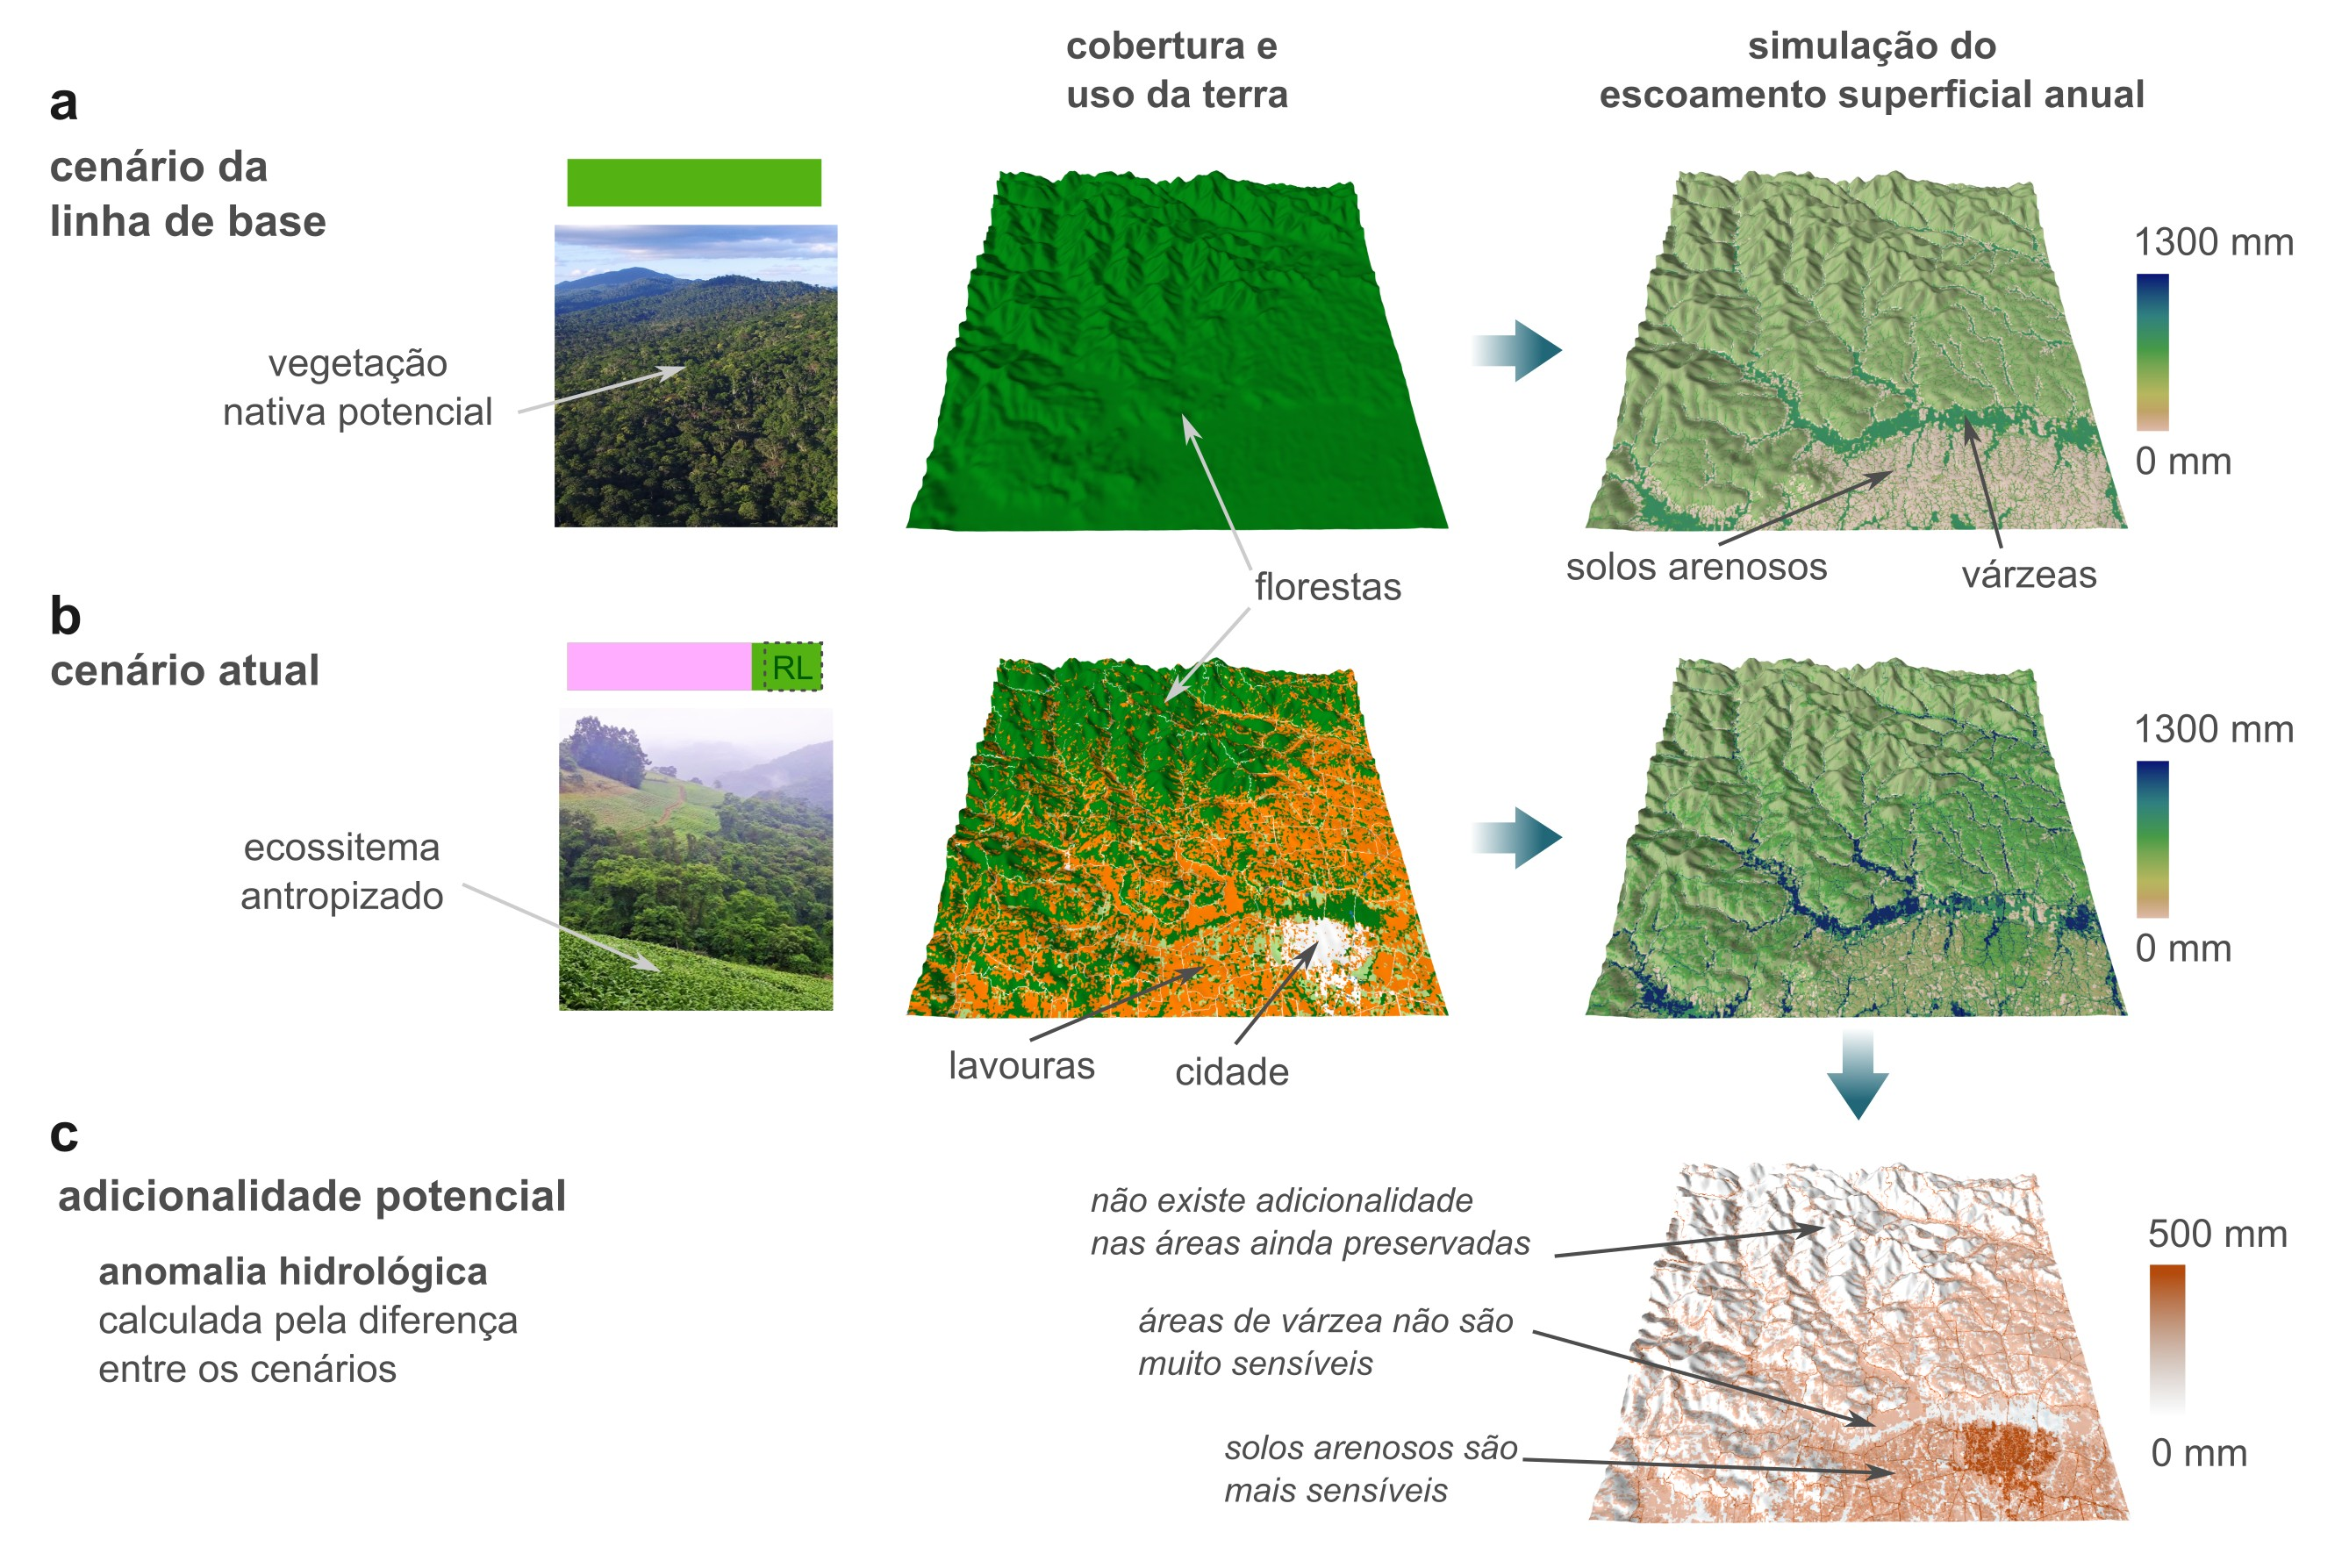
\includegraphics[width=0.98\linewidth]{figs/fig_addplans.jpg}		
\caption[Adicionalidade potencial com o modelo PLANS]
{\textbf{---\;A estimativa da adicionalidade potencial com o modelo PLANS.}
    Com o modelo PLANS, é possível estimar a adicionalidade potencial ao simular a hidrologia de bacias hidrográficas em cenários alternativos de uso da terra. Por ser baseado no TOPMODEL, o modelo considera não apenas solos e cobertura, mas também a influência dinâmica da topografia e áreas úmidas ripárias, o que é um diferencial considerando outros modelos. No exemplo, é ilustrado os resultados para a bacia hidrográfica do Arroio Castelhano, em Venâncio Aires, RS. Os mapas diários de escoamento superficial em 10 anos de simulações foram anualizados e comparados entre si.    
    \;\textbf{a}\;---\;O cenário da linha de base configurado como a vegetação nativa potencial. Nesse cenário de cobertura da terra uniforme, fica evidente que a parte da bacia com solos arenosos produz naturalmente menos escoamento superficial em função da condutividade hidráulica, enquanto que áreas úmidas ripárias produzem naturalmente mais escoamento superficial, em função da topografia.
    \;\textbf{b}\;---\;O cenário atual de cobertura da terra, com mosaicos de cidades, vias e lavouras, evidencia a maior produção de ecoamento superficial na bacia inteira, principalmente em função da menor capacidade de infiltração.    
    \;\textbf{c}\;---\;A diferença entre os cenários demonstra então a sensibilidade de cada parte da paisagem, mostrando que as áreas já preservadas não oferecem nenhuma adicionalidade. Da mesma forma, as áreas úmidas ripárias oferecem pouca adicionalidade. Áreas de lavoura em solos arenosos, por outro lado, são muito mais sensíveis, sendo um atrativo para a priorização de ações.
}
\label{fig:eco:addplans1} 		
\end{figure}

\par O modelo \texttt{PLANS}, desenvolvido em colaboração entre mim e demais colegas (ver Seção \ref{sec:hydro:plans}), surge como uma alternativa aos modelos \texttt{SWAT} e \texttt{InVEST}, amplamente utilizados na modelagem de serviços hidrológicos naturais (Francesconi \textit{et al.}, 2016 \cite{Francesconi2016}; Possantti \textit{et al.}, 2023 \cite{Possantti2023a}). O modelo \texttt{SWAT} adota uma abordagem que simula diversos processos hidrológicos considerando unidades de resposta hidrológica, a rede de drenagem e sub-bacias hidrográficas \cite{Strauch2013}. Em contraste, o modelo \texttt{InVEST}, particularmente em seu módulo de balanço hídrico, utiliza mapas de alta resolução espacial, embora os processos sejam simplificados em escala anual \cite{Daneshi2021a}. Assim, enquanto o \texttt{SWAT} oferece um maior detalhamento conceitual dos processos, o \texttt{InVEST} prioriza uma resolução espacial mais refinada \cite{Cong2020a}. O modelo \texttt{PLANS}, por sua vez, combina esses dois atributos: detalhamento conceitual e alta resolução espacial. Essa integração de atributos é possível em razão do modelo ser uma expansão da versão clássica do \texttt{TOPMODEL}, que define unidades de resposta hidrológica com base em atributos topográficos, conferindo ao modelo nuances espaciais detalhadas.

\begin{figure}[t!] 
\centering				
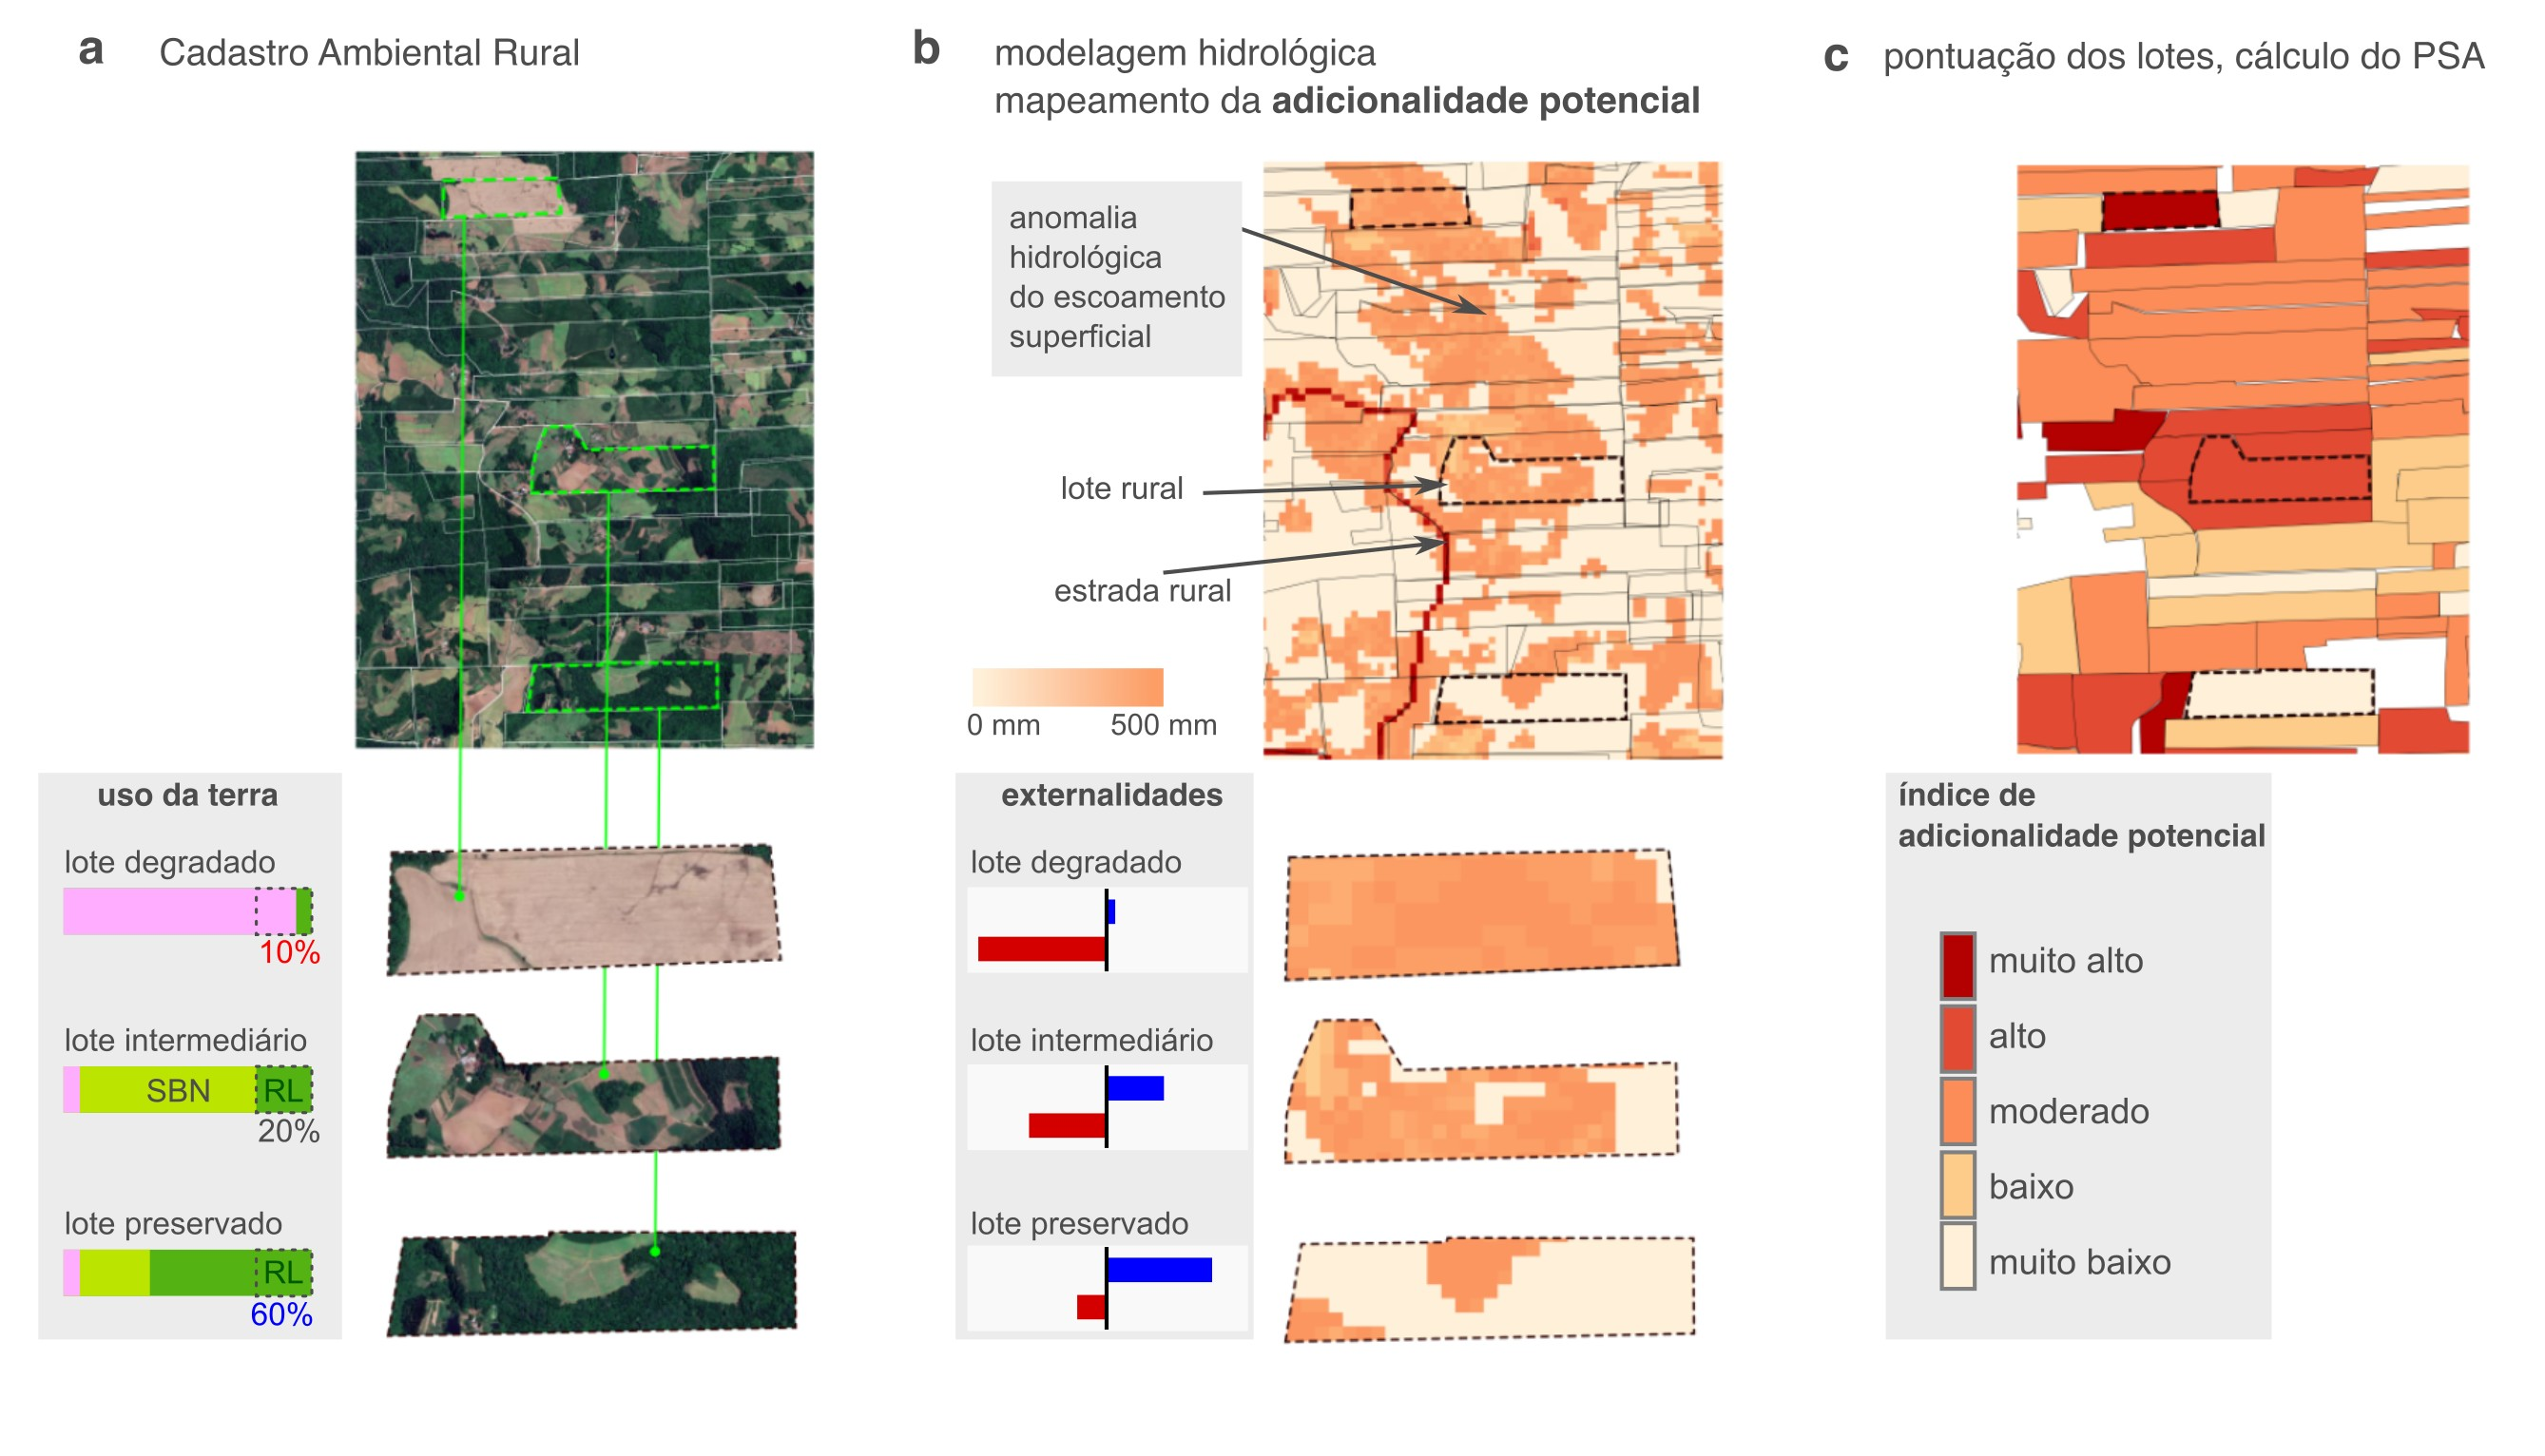
\includegraphics[width=0.98\linewidth]{figs/fig_lotscale.jpg}		
\caption[Adicionalidade na escala operacional dos lotes]
{\textbf{---\;Avaliando a adicionalidade potencial na escala operacional dos lotes.}
    Outro diferencial do modelo PLANS consiste na capacidade de produzir resultados em alta resolução espacial, o que favorece a estimativa da adicionalidade potencial na escala operacional dos lotes rurais. Essa vantagem decorre principalmente da sua organização em unidades de resposta hidrológica mais detalhadas que os modelos convencionais. 
    \;\textbf{a}\;---\;O Cadastro Ambiental Rural oferece a divisão territorial dos lotes rurais, incluindo o plano individual da propriedade. Aliado com sensoriamento remoto de alta resolução, é possível discernir lotes mais ou menos degradados.    
    \;\textbf{b}\;---\;Os resultados do modelo PLANS contribuem para se estimar a adicionalidade potencial de cada lote, o que oferece uma noção da magnitude da externalidade negativa que cada lote produz para jusante.    
    \;\textbf{c}\;---\;A adicionalidade potencial de cada lote pode então ser agregada em termos de índices de prioridade, contribuindo no planejamento de ações em esquemas de PSA.
}
\label{fig:eco:addplans2} 		
\end{figure}

\par Em relação ao mapeamento da adicionalidade potencial, ilustrada na Figura \ref{fig:eco:addplans1}, a simulação da hidrológica de cenários de cobertura do solo com o modelo \texttt{PLANS} na bacia hidrográfica do Arroio Castelhano (383 km²), em Venâncio Aires, permitiu se estimar uma capacidade de redução média no escoamento superficial em torno de 20\% (200 mm/ano) e um aumento no escoamento de base de aproximadamente 25\% (80 mm/ano), o que implica mil litros por segundo a mais de água relativamente perene e mais limpa no curso d´água. Os mapas anualizados mostram o padrão da anomalia hidrológica, especialmente nas áreas antropizadas onde a cobertura da terra tem maior influência. Nas regiões de cabeceiras montanhosas e mais preservadas com florestas de Mata Atlântica, a anomalia é mais baixa ou até inexistente. Entre as áreas antropizadas, uma região com solos arenosos demonstrou maior sensibilidade, pois, nas condições de referência, o escoamento superficial foi praticamente inexistente devido à alta condutividade hidráulica desses solos. Além disso, o modelo evidenciou que, nas áreas de talvegues e zonas úmidas ripárias, onde a topografia tem mais influência, a anomalia hidrológica é relativamente mais baixa. Nesses locais, a geração de escoamento superficial mostra-se menos dependente da cobertura e uso da terra, independentemente de serem áreas naturais ou antropizadas. Essa sensibilidade não é capturada em modelos hidrológicos como o modelo \texttt{SWAT} e \texttt{InVEST}, que não representam o fenômeno da área de contribuição variável.

\par Pelo lado da resolução espacial, o modelo \texttt{PLANS} oferece a capacidade de avaliar a adicionalidade potencial interna de cada lote rural, ou seja, na escala operacional adequada para diferenciar os lotes entre si. A principal razão para isso decorre da representação da influência da topografia, que permite a reconstrução de mapas detalhados dos processos hidrológicos simulados com precisão espacial. Dessa forma, lotes rurais com o mesmo tipo de solo e classe de cobertura, mas posicionados em diferentes partes da paisagem (como uma encosta e uma várzea, por exemplo), podem apresentar adicionalidades potenciais distintas, em função dos diferentes mecanismos de geração de escoamento predominantes. É importante destacar que os limites dos lotes rurais, disponíveis pelo Cadastro Ambiental Rural, são uma fonte essencial de dados para o desenvolvimento dos Planos Individuais da Propriedade (PIP), aplicáveis tanto em programas de PSA quanto no contexto de instrumentos de comando e controle, como a fiscalização das normas do Código Florestal. A integração com esse cadastro na modelagem da adicionalidade potencial, portanto, é uma vantagem relevante do modelo \texttt{PLANS} para mapear áreas prioritárias e calcular objetivamente a pontuação dos lotes candidatos em calculadoras de PSA, observando também o princípio da transparência. Mapas suficientemente detalhados que mostram os lotes rurais e seus diversos atributos ambientais, incluindo os hidrológicos, reforçam a confiança entre todas as partes envolvidas. 

\begin{figure}[t!] 
\centering				
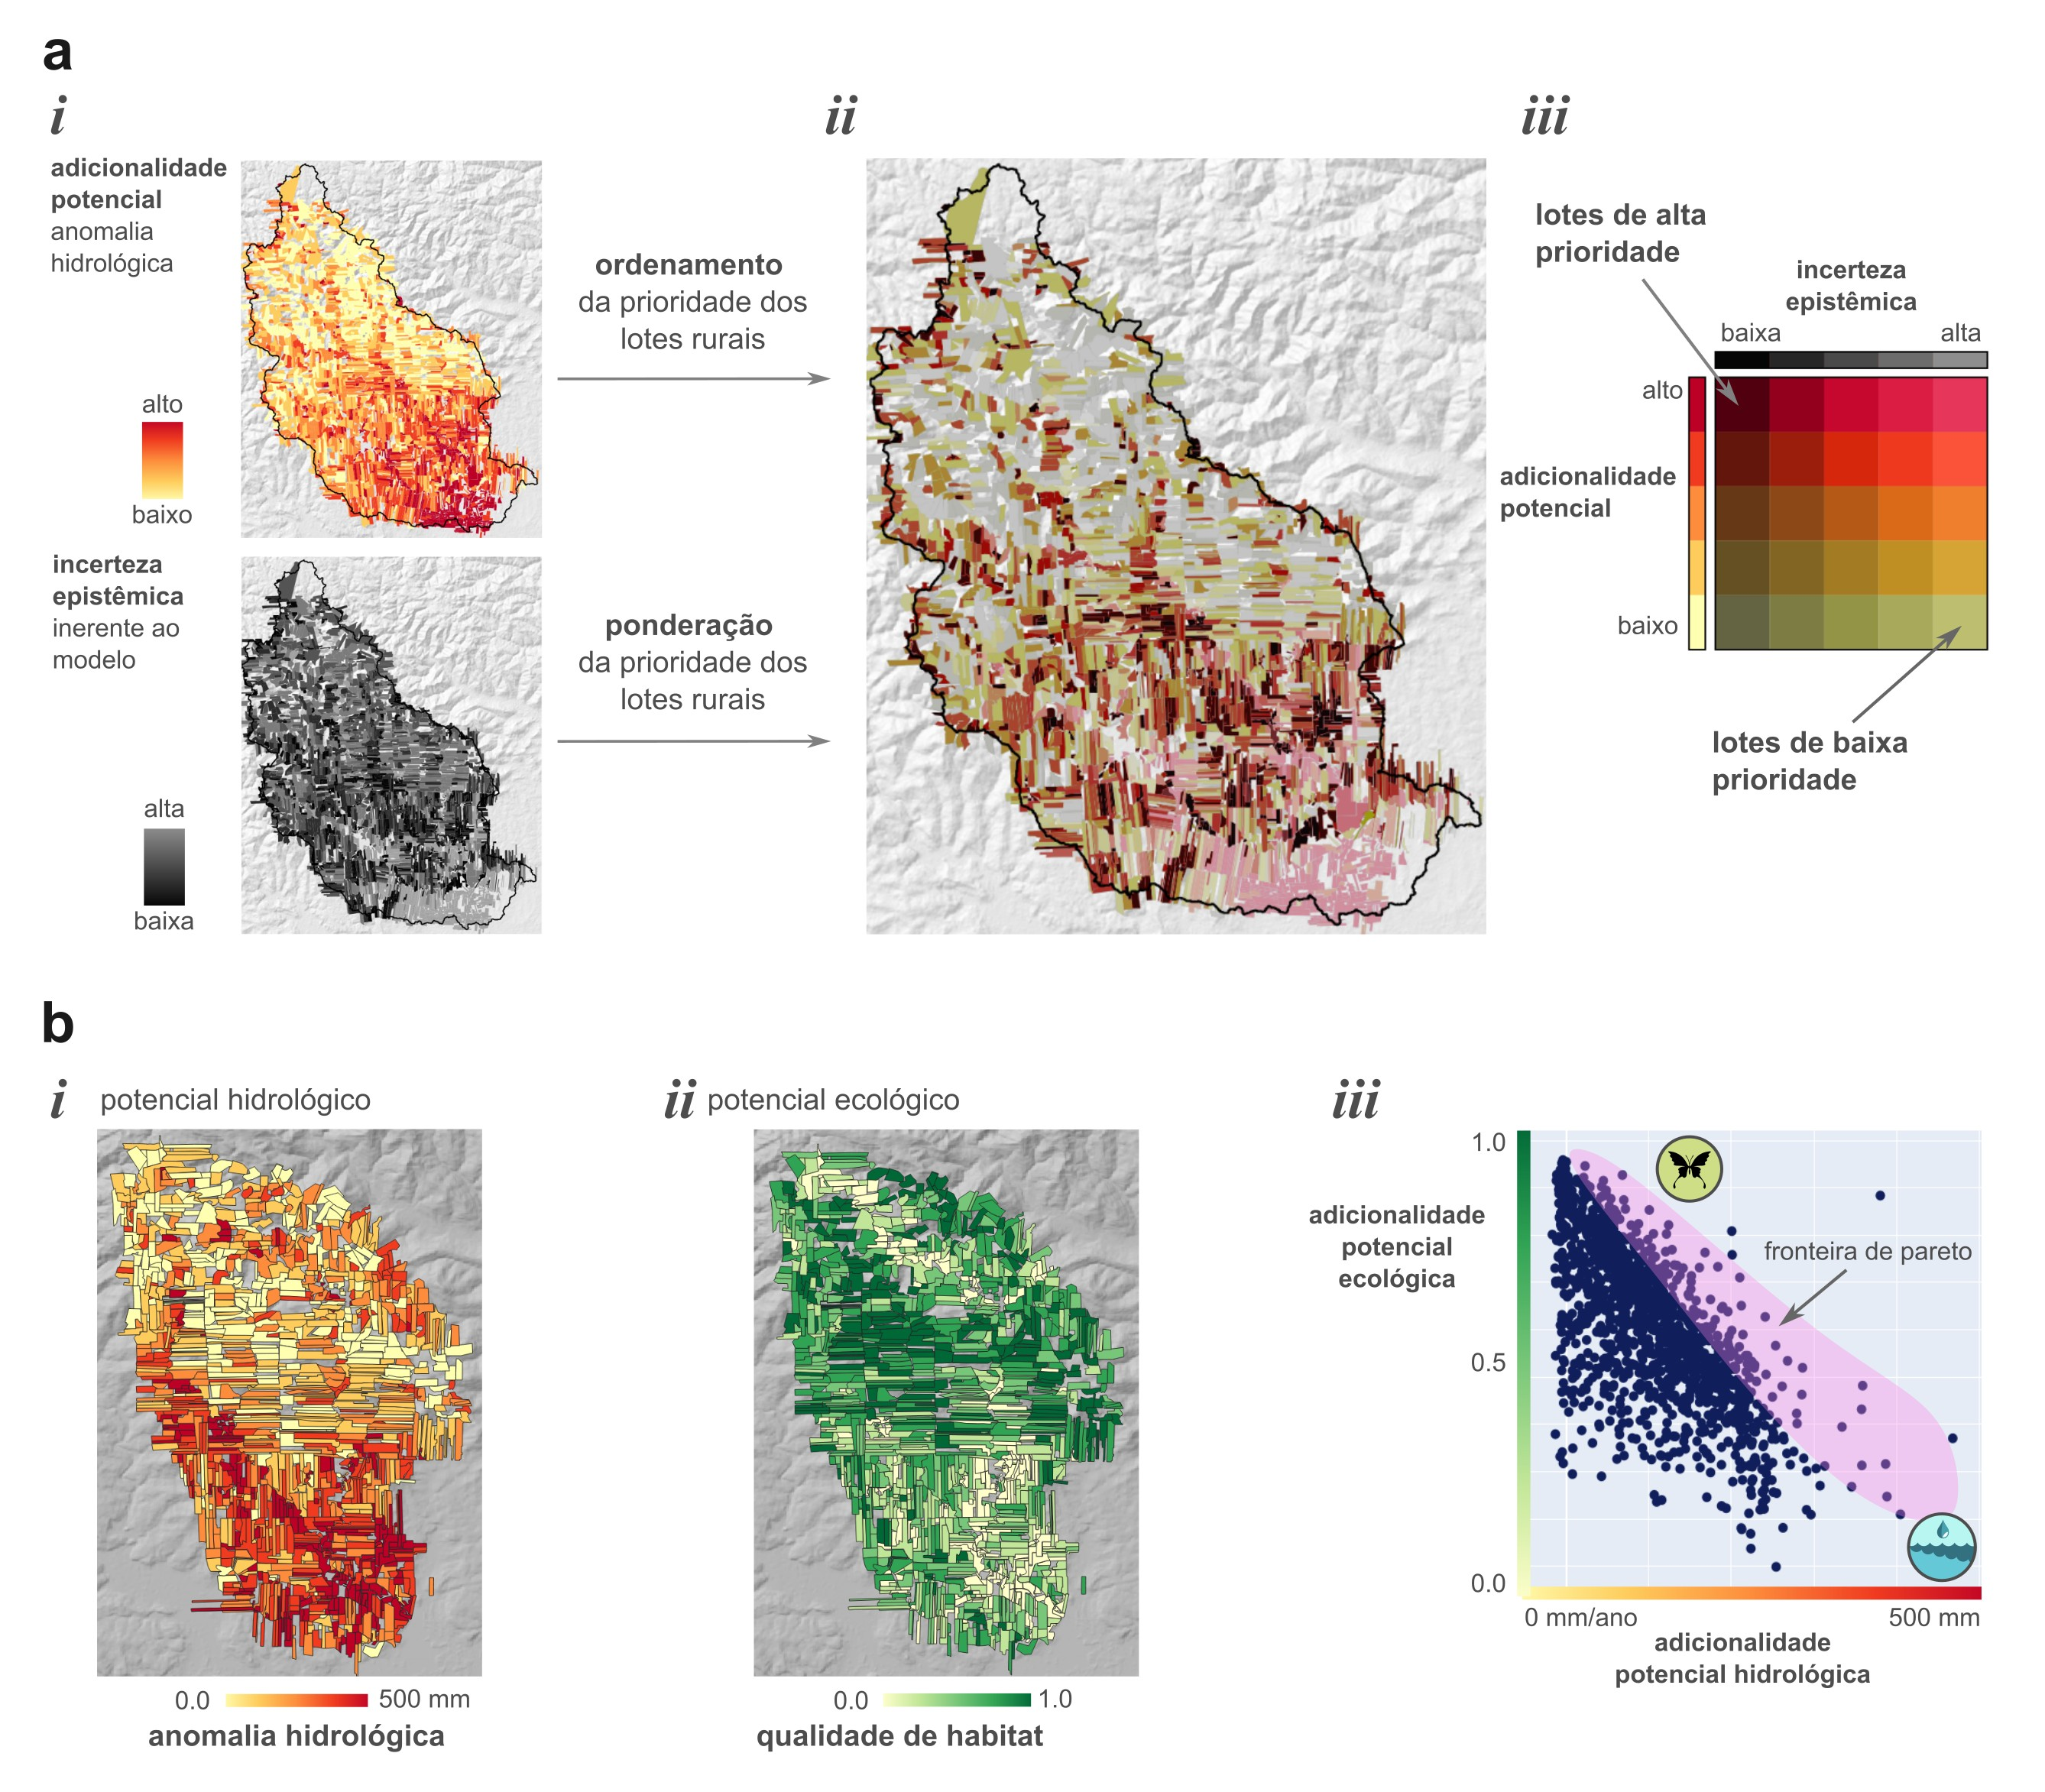
\includegraphics[width=0.98\linewidth]{figs/fig_index.jpg}		
\caption[O índice de prioridade e trade-offs]
{\textbf{---\;O índice de prioridade e avaliação de trade-offs.}
    Aplicações com o modelo PLANS abrem caminhos para assimilar incertezas e avaliar trade-offs.
    \;\textbf{a}\;---\;Um índice de prioridade de lotes rurais com base em modelos como o PLANS devem considerar as incertezas espaciais das simulações (detalhe \textrm{\textit{i}}). As bandas de incerteza do espaço, assim, funcionam como ponderadores do ordenamento, produzindo um índice de prioridade (detalhe \textrm{\textit{ii}}) que reflete tanto a atratividade de desempenho (maior adicionalidade potencial) quando a confiabilidade da estimativa (menor incerteza, detalhe \textrm{\textit{iii}})   
    \;\textbf{b}\;---\;Outros resultados de modelos ecológicos, como o Habitat Quality do modelo \texttt{InVEST} podem ser acoplados em uma análise abrangente, que considera sinergias e tradep-offs. No caso ilustrado na bacia do Arroio Grande (Venâncio Aires), o potencial de adicionalidade hidrológica se manifestou nas partes mais baixas da bacia, onde os lotes rurais são mais degradados. Por outro lado, a qualidade de habitat oferece um potencial de adicionalidade ecológica, pois vale mais a pena restaurar fragmentos de ecossistemas onde já está mais preservado. Essa dicotomia entre prioridades resulta em uma análise de perdas e ganhos (trade-offs), onde os melhores lotes localizam-se em uma fronteira de pareto.
}
\label{fig:eco:addplans3} 		
\end{figure}

\par Por fim, a aplicação do modelo \texttt{PLANS} na bacia hidrográfica do Arroio Castelhano incorporou as incertezas inerentes à modelagem hidrológica (detalhadas no Capítulo 1; ver Destaque \ref{box:uncert}). Para isso, incluiu-se, na construção do índice de prioridade, a ponderação pela dispersão dos modelos empiricamente adequados gerados pelo método GLUE, em conjunto com um algoritmo de busca (ver Destaque \ref{box:glue} para mais informações). Dessa forma, os lotes prioritários são definidos como aqueles com maior potencial de adicionalidade e menor incerteza associada. Essa abordagem também pavimenta novos caminhos, como a avaliação de trade-offs e múltiplos serviços-alvo, como recomendam as diretrizes de Naeem \textit{et al.} (2015). Por exemplo, a Figura \ref{fig:eco:addplans3} também mostra uma avaliação entre a adicionalidade potencial hidrológica e a adicionalidade potencial ecológica. Em geral, esses dois indicadores não coincidem, formando uma \textbf{fronteira de pareto} entre os serviços. Isso ocorre porque, em termos ecológicos, o potencial de adicionalidade é maior onde há menor fragmentação dos ecossistemas nativos, favorecendo ações prioritárias em lotes \textit{mais preservados} do que os lotes degradados, como no caso do potencial hidrológico. Com essas contribuições, o modelo \texttt{PLANS} busca integrar o processo de modelagem hidrológica desde seus fundamentos mais filosóficos com as suas consequências mais operacionais, proporcionando um arcabouço metodológico robusto e cientificamente rigoroso para guiar a transição para o desenvolvimento sustentável nas décadas que estão por vir. $\blacksquare$

\clearpage

\section{Resumo do capítulo}

\par Lorem ipsum dolor sit amet, consectetur adipiscing elit. Sed ac bibendum orci. Cras erat elit, consequat vel erat ac, tincidunt pulvinar lacus. Pellentesque vitae consectetur quam. Interdum et malesuada fames ac ante ipsum primis in faucibus. Curabitur at mollis eros. Integer ornare erat neque, id finibus velit ultrices in. Suspendisse dapibus tortor eget lorem pretium venenatis.

\begin{itemize}
    
    \item[$\blacksquare$] Lorem ipsum dolor um et malesuada fames ac ante ipsum primis in faucibus. Curabitur at mollis eros. Integer ornare erat neque, id finibus velit ultrices in. Suspendisse dapibus tortor eget lorem pretium venenatis.
    
    \item[$\blacksquare$] Lorem ipsum dolor sit amet, consectetur adipiscing elit. Sed ac bibendum orci. Cras erat elit, consequat vel erat ac, tincidunt pulvinar lacus. Pellentesque vitae consectetur quam. Interdum et malesuada fames ac ante ipsum primis in faucibus. Curabitur at mollis eros. Integer ornare erat neque, id finibus velit ultrices in. Suspendisse dapibus tortor eget lorem pretium venenatis.
    
    \item[$\blacksquare$] Lorem ipsum dolor sit amet, consectetur adipiscing elit. Sed ac bibendum orci. Cras erat elit, consequat vel erat ac, tincidunt pulvinar lacus. Pellentesque vitae consectetur quam. Interdum et malesuada fames ac ante ipsum primis in faucibus. Curabitur at mollis eros. Integer ornare erat neque, id finibus velit ultrices in. Suspendisse dapibus tortor eget lorem pretium venenatis.
    
    \item[$\blacksquare$] Lorem ipsum dolor sit amet, consectetur adipiscing elit. Sed ac bibendum orci. Cras erat elit, consequat vel erat ac, tincidunt pulvinar lacus. Pellentesque vitae consectetur quam. Interdum et malesuada fames ac ante ipsum primis in faucibus. Curabitur at mollis eros. Integer ornare erat neque, id finibus velit ultrices in. Suspendisse dapibus tortor eget lorem pretium venenatis.
\end{itemize}


\end{document}